\documentclass[11pt,a4paper,twoside,openright]{report}

% Document based upon the 'Report' class. 
% Uses 11pt text in standard font families, paper size is globally set to A4, the PDF will be laid out as a two-sided 
% document (allows different margins on odd/even pages for later binding) and its first page will be a right page. 

\includeonly{%		% comment out lines to not compile these sections when typesetting. 
	%%Preface
	./Preface/frontspace,%
	./Preface/copyright,%
	./Preface/dedication,%
	./Preface/toc,%
	./Preface/acknowledgements,%
	./Preface/abstract,%
	./Preface/sommario,%
	%
	%%Body
	%
	./chapters/intro,%
	./chapters/materials,%
	./chapters/synthesis,%
	./chapters/characterization,%
	./chapters/fabrication,%
	./chapters/dataAnalysis,%
	./chapters/results,%
	./chapters/conclusion,%
	./chapters/appendix
	}

%%%%%%%%%%%%%%%%%%%%%%%%%%%%%%%%%%%%%%%%%%
%%%%%%%%%% PACKAGE MANAGEMENT %%%%%%%%%%%%%%%%%%
%%%%%%%%%%%%%%%%%%%%%%%%%%%%%%%%%%%%%%%%%%

\usepackage{soul}
\usepackage{color}
\usepackage{graphicx}	% Package for using images (.jpg, .pdf, .png, etc.) as figures. 
\usepackage[center]{caption}	% Captioning packages for floats (figures, tables, etc.). '[Center]' forces centering
\usepackage{subfig}
%\usepackage{subcaption}	% Allows for sub-figures to have their own sub-captions, shouldn't be in TOC
\usepackage{tabularx} % Allows for automatic sizing for tabular environments (see CTAN for manual)
\usepackage[super]{cite}	% Automatic citation generation package '[super]' forces superscript citations
\usepackage{afterpage}	% Package to be used with \clearpage to help keep floats from drifting to end of document. (See CTAN for manual)
%\usepackage[version=3]{mhchem}	% Automatic formatting of chemical equations and formulas
\usepackage[method=mhchem]{chemmacros}
\usepackage{amsmath,amssymb,mathtools}	%Packages for various equation tools
\usepackage{rotating}	% Allows rotation of objects (figures, tables, etc.). Preferable to use landscape environment in most cases (\begin{lscape})
\usepackage{xnewcommand}
\usepackage{siunitx}
\usepackage{fancyhdr}	% Package for setting up headers and footers
\usepackage[english]{babel}	% Language setting, not sure why its necessary, but is.
\usepackage[nodayofweek]{datetime}	% Allows for proper determination of date
\usepackage{etoolbox} 	% Unimportant for end user. 
\usepackage{lipsum}	% Allows for automatic creation of filler text. 
\usepackage[margin=3.5cm]{geometry}	% Defines page layout geometry
\usepackage{lscape}	% Allows pages to be defined as landscape (environment)
\usepackage{indentfirst}	% Forces an indent on all paragraphs, including first paragraphs. 
\usepackage{empheq}	% Used to add braces to groups of equations
\usepackage[running,modulo]{lineno}	% Adds line numbers (only multiples of 5) to left side margin
\usepackage{varioref}
\usepackage{multirow}
\usepackage{longtable}
\usepackage{booktabs}
\usepackage{arydshln}

% Hyperref package: used for setting up hyperlinks in the document (TOC, citations, figures, equations, etc.), as 
% well as adding PDF metadata (author, title, etc.)
\usepackage[pdftex,%	Informes explicitly use of pdftex for document preparation engine
		      hyperfigures, % 	Requests hyperlinks from figure citations to their associated figures
		      pageanchor=true,% 	Necessary for proper hyperlinking of TOC
		      %pagebackref=true,%
		      hyperindex=true,%	If index is present, entries will link back to the first appearance of the term
		      colorlinks=true,%	Colors links in document (internal: red, citations: green)
		      bookmarks=true,%	Creates bookmarks list in the final PDF
		      bookmarksnumbered=true,%	Adds chapter number to the associated bookmark
		      bookmarksopen=true,%	All bookmark trees open when PDF opened, not working
		      pdftitle={Atomic Layer Deposition of Ferroelectric Complex Oxide Thin Films},%	Document title
		      pdfauthor={Brian R. Beatty},%	Document author
		      pdfsubject={M.S. Thesis},%	Document subject
		      pdfkeywords={ALD, Atomic Layer Deposition, Ferroelectric, Complex Oxide, Perovskite,%
		      			     Lead Titanate, Ellipsometry, PbTiO3, PTO},%	List of keywords for document
		      ]{hyperref}	


%%%%%%%%%%%%%%%%%%%%%%%%%%%%%%%%%%%%%%%%%%
%%%%%% ADJUSTS CHAPTER TITLES CLOSER TO HEADER   %%%%%%%%%
%%%%%%%%%%%%%%%%%%%%%%%%%%%%%%%%%%%%%%%%%%

\makeatletter
% "\@makechapterhead" applies to ordinary or numbered chapters
\patchcmd{\@makechapterhead}{\vspace*{50\p@}}{}{}{}
\patchcmd{\@makechapterhead}{\vskip 40\p@}{\vskip 20\p@}{}{}
% "\@makeschapterhead" applies to "starred" or un-numbered chapters
\patchcmd{\@makeschapterhead}{\vspace*{50\p@}}{}{}{}
\patchcmd{\@makeschapterhead}{\vskip 40\p@}{\vskip 20\p@}{}{}
\makeatother

\widowpenalty=500
\clubpenalty=500



%%%%%%%%%%%%%%%%%%%%%%%%%%%%%%%%%%%%%%%%%%
%%%%%%%%%%% MISCELLANEOUS ADJUSTMENTS   %%%%%%%%%%%%
%%%%%%%%%%%%%%%%%%%%%%%%%%%%%%%%%%%%%%%%%%

\setlipsumdefault{1-2}  % Makes \lipsum automatically produce 2 paragraphs of filler text

\renewcommand{\lipsum}{} % Hide dummy text paragraphs

\renewcommand{\captionfont}{\normalfont \sffamily \itshape \small}
%\renewcommand{\contentsname}{Table of Contents}

\pagestyle{empty} % Sets pages to have no header/footer. Will be changed later in the document. 


%%%%%%%%%%%%%%%%%%%%%%%%%%%%%%%%%%%%%%%%%%
%%%%%%%%%%% LAYOUT GEOMETRY ADJUSTMENTS  %%%%%%%%%%%
%%%%%%%%%%%%%%%%%%%%%%%%%%%%%%%%%%%%%%%%%%

%\addtolength{\oddsidemargin} {-0.4 cm} 	% Shrinks the side margins slightly.
%\addtolength{\evensidemargin} {-0.4 cm}	% Shrinks the side margins slightly. 

\setlength{\headheight}{26pt} 	% Changes the size of the header (the console will complain if it's too small).

\linespread{1.25} 	% Changes line spacing



%%%%%%%%%%%%%%%%%%%%%%%%%%%%%%%%%%%%%%%%%%
%%%%%%%%%%%  CHEMICAL EQUATION FORMATTING  %%%%%%%%%%%
%%%%%%%%%%%%%%%%%%%%%%%%%%%%%%%%%%%%%%%%%%

\renewtagform{reaction}[R ]{(}{)}


%%%%%%%%%%%%%%%%%%%%%%%%%%%%%%%%%%%%%%%%%%
%%%%%%%%%  PERSONALIZED COMMANDS %%%%%%%%%%%%%%%%%
%%%%%%%%%%%%%%%%%%%%%%%%%%%%%%%%%%%%%%%%%%

% Shortcuts for typesetting certain things quickly (saves time when typing things often). 
% Always use an empty set of braces after the command unless it has arguments. 

\newcommand{\PTO}{\ce{PbTiO3}}

\newcommand{\PZT}{\ce{PbTi_{1-x}Zr_{x}O3}}

\newcommand{\Deg}{$^{\circ}$}
\newcommand{\degC}{$^{\circ}$C}
\newcommand{\Tc}{T$\mathrm{_{C}}$}

\newcommand{\TiIon}{\ce{Ti^{4+}}}
\newcommand{\OIon}{\ce{O^{2-}}}
\newcommand{\PbIon}{\ce{Pb^{2+}}}
\newcommand{\ZrIon}{\ce{Zr^{4+}}}
\newcommand{\TiOiPr}{Ti-o-\emph{i}-Pr}

\newcommand{\TMHD}{Pb(TMHD)$_{2}$}
\newcommand{\tmhd}{\TMHD}
\newcommand{\HFAc}{Pb(HFAc)$_{2}$}
\newcommand{\hfac}{\HFAc}

\newcommand{\leftstuff}[2][0pt]{\smash{\raisebox{#1}{\llap{#2}}}}

\newcommand{\reword}[1]{%
	\sethlcolor{yellow}%
	\hl{#1}%
	}

\newcommand{\rewrite}[1]{\reword{#1}}

%%%%%%%%%%%%%%%%%%%%%%%%%%%%%%%%%%%%%%%%%%
%%%%%%%%%%% DOCUMENT STARTS HERE  %%%%%%%%%%%%%%%%
%%%%%%%%%%%%%%%%%%%%%%%%%%%%%%%%%%%%%%%%%%

\begin{document} 	% Now the fun starts.

%%% PREFACE %%%

\thispagestyle{empty} % No headers/footers allowed here
\thispagestyle{empty}
\begin{titlepage}
\vspace*{-3cm}
\begin{center}
  {\LARGE
  \textsc{Politecnico di Milano}\\
  \textbf{\Large
  Facolt\`a di Ingegneria dei Processi Industriali}\\
  \emph{\large Degree in Materials Engineering and Nanotechnology}}\\
  \vspace*{0.5cm}
  \begin{figure}[htbp]
    \begin{center}
      
\includegraphics[width=5cm]{./pictures/logopm.png}
    \end{center}
  \end{figure}
  \vspace{-0.3cm}
   {\huge\textsc{
  Atomic Layer Deposition of \\
  Ferroelectric Complex\\Oxide Thin Films\\
  }}

  
  
\end{center}
\vspace{0.3cm} 
\large
\begin{flushleft}

\begin{tabular*}{0.75\textwidth}{>{\bfseries}r l}
  Advisor & Dr. Jonathan E. Spanier \\
  & \emph{\small Drexel University, Philadelphia, Pennsylvania, United States of America}\\
  Co-Advisor  & Dr. Carlo S. Casari \\
  & \emph{\small Politecnico di Milano, Milano, Italia}
  \vspace{0.3cm}
%  Co-Advisor  & Dr. Spain Advisor \\
%  & \emph{\small Universidad Polit\'ecnica de Madrid, Madrid, Espa\~na}\\
\end{tabular*}


\end{flushleft}
%\vspace*{0.5cm}
\rule{\linewidth}{0.5mm}
\begin{centering}

  {\small{\Large\scshape Master's Thesis}\\Presented in\\{\Large\scshape Partial Fulfillment}\\of the\\{\Large\scshape Requirements for the Degree}\\of\\{\Large\scshape Master of Science}\\by:\\}
  \vspace*{0.5em}\textbf{\LARGE Brian R. Beatty}\\ \vspace*{0.5em}\small Matricola: 780703 \\ 
\vspace*{1em}
\rule{\linewidth}{0.5mm}

\end{centering}
\vspace*{0.5cm}
\begin{center}



  Academic Year 2011-2012
\end{center} \clearpage

\end{titlepage} % Opens a sub-TEX file. ./ is the current local directory. 

\thispagestyle{empty} \normalfont \cleardoublepage  % No header/footer on this page, then starts new odd # page
\vspace*{\fill}

\begin{center}

\copyright\ Copyright \monthname\ 2012\\
Brian R. Beatty. All Rights Reserved.

\end{center}

\vspace*{\fill}

\thispagestyle{empty} \normalfont \cleardoublepage
\newpage
\vspace*{4cm}
\large
\begin{flushright}
\itshape{For my parents and everyone\\else who helped out along the way...}
\end{flushright}


\thispagestyle{empty}  \cleardoublepage

\linenumbers	% Starts numbering of document lines
\pagenumbering{roman} %Start numbering preface pages using roman numerals (i, ii, iii, iv, ...)

\tableofcontents
\label{toc:ToC}
\captionsetup{lofdepth=2}

\listoffigures
\label{toc:listoffig}
\addcontentsline{toc}{chapter}{List of Figures}

\cleardoublepage
\thispagestyle{empty}
\listoftables
\label{toc:listoftbl}
\addcontentsline{toc}{chapter}{List of Tables}
%\listofreactions
%\addcontentsline{toc}{chapter}{List of Reactions}

% Uncomment below to add a list of tables. Probably necessary for sample information table. 

%\label{toc:listoftbl}
%\listoftables
%\addcontentsline{toc}{chapter}{List of Tables}
\thispagestyle{empty} \vspace*{.75truecm} \cleardoublepage

\chapter*{Acknowledgements}

\addcontentsline{toc}{chapter}{Acknowledgements}

I would like to start by acknowledging Dr. Jonathan Spanier for all of the all of the guidance that he has given to me over the course of my tenure at Drexel University. Allowing me to enter into the research side of school as a young freshman with stars in his eyes was undeniably one of the defining points in my academic career. The variety of skills I have been able to learn while working with him, and of course all of the members of his extremely talented group, are sure to prove to be invaluable during the next stages of life after Drexel. While I learned plenty of facts and received valuable training in an incredible range of technical equipment, what really stands out is the manner in which I was taught how to think. How to think about puzzling results that didn't quite add up evenly. How best to plan experiments to maximize the data obtained from it. Analyzing the remnants from when things went wrong, and figuring out how to prevent such things from happening in the future. The researcher's mindset is one of inquisitiveness and analysis and a drive to truly understand, and it has been of great value both in and out of the laboratory. 

Another pair of honorable mentions goes to Dr. Stephen Nonnenmann and Dr. Eric Gallo. These two would act as mentors as I tried to get my feet under me in my first year or so. Always around to bounce questions off of, quick with helpful advice, and utterly filled to the brim with useful knowledge. Between these two, there was nothing that couldn't get done or be answered in the lab. These two set me up with the knowledge and mental tools I would need to go off exploring on my own journeys into the wild seas of science. I cannot thank them enough. 

Then there was the rest of the stalwart crew. Stephanie Johnson, Oren Leaffer, Terrance McGuckin, Guannan Chen, and Christopher Hawley. And I couldn't forget my fellow undergrads Dominic Bruzzese and Michael Coster. The great conversations --- especially with Oren (whom I can still count on for some useful advice about any question) even if they tended to get a little long-winded at times --- that I had with these characters will be some of my best memories from my time here. Each of us had our own idiosyncrasies, but I like to think we made a fantastic team when you put us all together. 

Of course, I would also like to send a heartfelt thank you to three more individuals who worked closely with my project at three very different stages. Rahul Joseph was my mentor when I first joined the lab, and it was a derivative of his project that over time metamorphosed into the thesis sitting before you.  Dr. Greg Soja was a post-doctorate fellow who worked alongside me on this project as well, and helped solve some rather difficult problems that we encountered. Last, but far from least, is Dr. Maria Sancho-Torres. She brought a bit of spark and a new point of view to the project that, again, helped sort out some problems that otherwise might have stymied me for a lot longer than they should have. 

I must also thank Keith Fahnstock and Dr. Caroline Schauer for allowing me and helping me with the use of their ellipsometer. Keith in particular, for his training and just good conversation (both on and off topic) when data collection got boring. In the same vein, I must gratefully acknowledge the assistance that Dr. Amy Fahnstock and her advisor Dr. Giuseppe Palemese provided me by allowing access to their TGA and DSC instrumentation that was pivotal to the success of this project. 

Of course, one does not live in a bubble, and I must thank the rest of the excellent faculty of the Materials Engineering Dept. for all of their efforts (both for their informative courses, but primarily for the discussions we had outside the classroom). I feel that I need to particularly acknowledge Dr. Steve May and Dr. Antonios Zavaliangos in this regard. 

Along the lines of the opportunity I have had during this past year abroad, I would like to personally thank Dr. Carlo Casari, Politecnico di Milano, and everyone who had a hand in making the E.A.G.L.E.S. program come together. And of course the scores of crazy friends that I picked up along the way. 

This has been a lot of talk already, but I personally feel I saved the most important for last.  My father, Bruce, and my mother, Amy, deserve more thanks than I think they realize. For being the supports that I could fall back on, for sharing in both the little successes and the big triumphs, for always letting me talk about what I was working on (and oh the respect I have for trying to learn about it from me...), and for always pushing me to go beyond what I thought I was capable of. Mom and Dad, thank you so very much. This one's for you guys. Now on with the show. 












\thispagestyle{empty} \vspace*{.75truecm} \normalfont \cleardoublepage

\newpage
\chapter*{Abstract}
\addcontentsline{toc}{chapter}{Abstract}

%%%%%%%%%%%%%%%%%%%%%%%%%%%%%%%%%%%%%%%%%%%%%%%%%%%%
%%%%%%%%%%%%%%%%%%%%%%%%%%%%%%%%%%%%%%%%%%%%%%%%%%%%
%%%%%%%%%%%%%%%%%%%%%%%%%%%%%%%%%%%%%%%%%%%%%%%%%%%%

\noindent Blah blah blah ferroelectric stuff. 

As devices based on ferroelectric films become more commonplace, a commercially viable process for fabricating the material is needed; low cost and high volume are implied necessities for such a process. This work focuses on the application of atomic layer deposition (ALD) to this task. ALD is a standard fabrication process in the electronics industry, valuable for its high uniformity across large surfaces, capability to control film thickness with very high resolution, and conformality across three dimensional structures. The various tasks in designing and optimizing an ALD process, as well as characterization methods for analysis of the produced films, will be discussed in detail.

Work supported by ARO? under Grant \#.
\thispagestyle{empty} \vspace*{.75truecm} \cleardoublepage

\newpage
\chapter*{Sommario}

\addcontentsline{toc}{chapter}{Sommario}

\noindent this part has to be a detailed description of the project written completely in italian. sad face.
\thispagestyle{empty} \vspace*{.75truecm} \cleardoublepage

%%% END OF PREFACE %%%

\pagenumbering{arabic}  % Start numbering pages using arabic numerals (1, 2, 3, 4, ...)


%%%%%%%%%%%%%%%%%%%%%%%%%%%%%%%%%%%%%%%%%%
%%%%%%%%%%% HEADER/FOOTER SETUP  %%%%%%%%%%%%%%%%%
%%%%%%%%%%%%%%%%%%%%%%%%%%%%%%%%%%%%%%%%%%

\pagestyle{fancy} 	% Activates fancyhdr package to make customized headers/footers. 

\renewcommand{\chaptermark}[1]{\markboth{\chaptername\ \thechapter :\ #1}{}} % Changes definitions for chapter titles in header
\renewcommand{\sectionmark}[1]{\markright{\thesection :\ #1}}         % Changes definitions for section titles in header

\fancyfoot{}

\fancyhead[LE,RO]{\bfseries\thepage}    % Page number will be bold and appear on the left side on even pages (LE) and the right side on odd pages (RO).
                                        
\fancyhead[RE]{\bfseries\leftmark}    % Uses default settings for right page headers (chapter number and title)
\fancyhead[LO]{\bfseries\rightmark}     % Uses default settings for left page (section number and title
\renewcommand{\headrulewidth}{0.3pt} % Changes geometry settings



%%% BEGIN CONTENT %%%

% Each chapter located in its own sub-file to make it easier to work on them. NOTE: they will not compile on their own. 
% To view the result, you need to run TeX on the main document (thesis.tex). Can be done by clicking on the open 
% PDF and pressing command-T. 

% NOTE: 	To get references (to figures and such) to update properly, TeX must be run TWICE. 
% 	 	To get citations to work properly, you must run: TeX (cmd-T), BibTeX (cmd-shft-B), TeX, TeX. (4 total runs)

\chapter{Introduction}
\label{ch:Intro}
\thispagestyle{empty}


%%%%%%%%%%%%%%%%%%%%%%%%%%%%%%%%%%%%%%%%%%%%%%%%%%%
%%%%%%%%%%%%%%%%%%%%%%%%%%%%%%%%%%%%%%%%%%%%%%%%%%%
%%%%%%%%%%%%%%%%%%%%%%%%%%%%%%%%%%%%%%%%%%%%%%%%%%%

Modern technology stands on the shoulders of modern materials, and the two are inextricably linked together. Whenever a new material or property has been discovered or engineered, applications of this new capability lie just over the horizon. 

One of the hotbeds of innovation and interest in novel applications of material properties is the field of oxide chemistry. Such a seemingly simple class of materials, examples of which are two of the most abundant compounds on Earth (i.e. silica and alumina), has an incredibly rich set of capabilities derived from the incredible variety of potential materials. One example is the field of high-\textsc{k} dielectric oxides, such as hafnium oxide (\ce{HfO2}) and zirconium oxide (\ce{ZrO2}),\cite{chen_atomic_2007,fischer_batch_2008} which are allowing the semiconductor industry to produce more capable devices while reducing power draw. Ferromagnetic and antiferromagnetic oxides form the basis of the ubiquitous magnetic hard disk drive, advancements in deposition and microstructure control allow for the steady increase in capacities that consumers have become accustomed to.\cite{scheffe_atomic_2009}

The class of ferroelectric oxides comprises the family of materials that this thesis will consider. One material in particular will be the primary subject: lead titanate (PTO, \PTO{}).\cite{harjuoja_2006,lee_effects_2009} Lead titanate is one end group of the lead zirconate titanate family of ferroelectric oxides (PZT, \ce{PbZr_{1-x}Ti_{x}O3}).\cite{Muralt_2000} The PZT family is of particular technical importance to many applications, especially the \ce{PbZr_{0.52}Ti_{0.48}O3} form which exhibits exemplary piezoelectric, ferroelectric, and pyroelectric behavior. PZT's piezoelectric capabilities allow for it to be used as actuators and sensors in innumerable devices (e.g. tip actuators in AFM microscopes and transducers in ultrasound imagers). 

Other applications of such materials are found when they are created as nanoscale thin films, where these capabilities are both more strongly exhibited. One of the more prevalent methods of producing nanoscale films is chemical vapor deposition (CVD), a powerful process that has been used to deposit a vast number of material types and structures.\cite{Matsumara_1998}

However, there are disadvantages to the CVD method of film deposition. Great care must be taken to obtain highly regular film thicknesses, and the method of producing most oxide films --- a variation called metallorganic CVD (MOCVD) after the metallorganic compounds used as reactants --- allows a significant amount of hazardous material to be released into the environment as toxic and nano-particulate byproducts. 

Another deposition method, atomic layer deposition (ALD), is becoming popular in industry applications as an alternative to CVD. ALD provides the user with ultra-high resolution on film thickness, a lower operating temperature than nearly all CVD processes, amongst other features. In addition, due to the nature of the process, ALD is capable of consuming far less precursor material as well as utilizing a far larger percentage in depositing the film as opposed to producing the types of byproducts caused by CVD.\cite{ALD-Handbook} This makes ALD, in situations where it can be applied, the more economical choice, as well as being more sustainable and environmentally friendly. To this end, the National Science Foundation (NSF) has awarded funding (under 2012 grant \#1200940) toward the development of alternative ALD precursors, models, and processes that will attempt to provide additional improvements to the sustainability of ALD.

However, well described processes for producing ALD films of many materials have not been developed. Binary oxides (\ce{A_{x}O_{y}}) have been explored in a fair amount of depth,\cite{chen_atomic_2007,de_ridder_growth_2002,knez_atomic_2006,lee_al2o3_2003,scheffe_atomic_2009} but there is less research work available covering processes for depositing complex oxide films via ALD. 

%%%%%%%%%%%%%%%%%%%%%%%%%%%%%%%%%%%%%%%%%%%%%%%%%%
%%%%%%%%%%%%%%%%%%%%%%%%%%%%%%%%%%%%%%%%%%%%%%%%%%
%%%%%%%%%%%%%%%%%%%%%%%%%%%%%%%%%%%%%%%%%%%%%%%%%%

\section{Project Scope}
\label{sec:Intro-Scope}

This thesis will cover the main steps taken in developing a thin film deposition processes using ALD. In chapter~\ref{chap:Materials} lead titanate as a material will be introduced, discussing its structure and some of the desirable properties that the oxide exhibits due to this structure. 

Chapter~\ref{chap:Synth} will be devoted to a few of the commonly used methods used to produce films of complex oxides, sol-gel and MOCVD, as well as introducing in detail the primary focus of this project: the deposition of thin films via ALD. 

Following this, chapter~\ref{ch:SampFab} will go into detail of the various choices and parameters that go into the development of an ALD process. Concepts such as the choice of precursors from the various deposition parameters that must be carefully controlled and tuned to produce optimal results. 

Chapter~\ref{chap:Charact} will introduce and briefly discuss the topics involved in characterizing the various materials to be utilized in the deposition process, as well as the various techniques used to analyze and quantify the properties of the produced samples. 

Subsequently, chapter~\ref{ch:Methods} will go into more detail of exactly how these analyses were performed, briefly mentioning various details of the standard measurement techniques as well as going into a bit more detail where analysis procedures were developed for application to this project. 

In chapter~\ref{ch:Results}, the details of the results and data collected from the various measurements and experiments that were performed during this study will be discussed thoroughly.  

Finally, chapter~\ref{ch:Conc} will draw conclusions from the entirety of the work done in the course of this project, as well as discuss possibilities for future experimentation and refinement of the process. A prime example of this would be to apply this research into the development of a procedure to produce films composed of the far more technically relevant PZT(52-48). 


%
%The primary scope of this project involved the creation of a method to produce lead titanate thin films. To this end, a number of different steps needed to be taken. Primarily, 
\chapter{Lead Titanate}
\label{chap:Materials}
\thispagestyle{empty}


%%%%%%%%%%%%%%%%%%%%%%%%%%%%%%%%%%%%%%%%%%%%%%%%%%%
%%%%%%%%%%%%%%%%%%%%%%%%%%%%%%%%%%%%%%%%%%%%%%%%%%%
%%%%%%%%%%%%%%%%%%%%%%%%%%%%%%%%%%%%%%%%%%%%%%%%%%%

\section{Structure}
\label{sec:Materials-Struct}

Lead titanate (\PTO{}, PTO) naturally orders into the tetragonal perovskite crystal structure at room temperature (figure~\vref{fig:Crystals}). The structure can be affected by compositional changes, temperature, or strain (primarily in thin-film systems), allowing a transition to a cubic phase. In the perovskite crystal structure, the central cation (\TiIon{} in the case of \PTO{}) is encapsulated in a octahedral cage of anions (\OIon{}), with the remaining cations (\PbIon{}) situated in the eight corners of the unit cell. if the material was doped (as in a mixed solid-solution), some of the cations would be replaced with the dopant ions, for example \ZrIon{} would be randomly distributed in  \TiIon{} sites in the \PZT{} (PZT) system. 

%\begin{figure}[htb]
%   \begin{center}
%   \includegraphics[width=0.4\textwidth]{./figures/materials/pbtio3-crystal.pdf} 
%   \caption[Crystal structure of \PTO{}]{Tetragonal perovskite structure of \PTO{}. \\Grey, red, and blue spheres refer to \PbIon{}, %
%   		\TiIon{}, or \OIon{}, respectively}
%   \label{fig:PTO-crystal}
%   \end{center}
%\end{figure}

\begin{figure}[tbp]
   \centering
   \subfloat[][General Perovskite]{%
   	\label{fig:Perovskite-Crystal}%
	\includegraphics[width=0.4\linewidth]{./figures/materials/perovskite-crystal.pdf}%
	} 
   \hspace{0.5cm}	
   \subfloat[][Lead Titanate (\ce{PbTiO3})]{%
   	\label{fig:PTO-Crystal}%
	\includegraphics[width=0.4\linewidth]{./figures/materials/pbtio3-crystal.pdf}%
	} 	
   \caption[Crystal Structures of Perovskites and \ce{PbTiO3}]%
   		{The perovskite (\ce{ABO3}) crystal structure.\\(a) The general structure of perovskite oxides. %
		(b) Tetragonal asymmetric perovskite structure of \PTO{}. Grey, red, and blue spheres refer %
		to \PbIon{}, \TiIon{}, and \OIon{}, respectively. Additionally, the octahedral oxygen cage is %
		shown in pale blue. %
		}
   \label{fig:Crystals}
\end{figure}

%%%%%%%%%

\subsection{Effect of Temperature}

The transition from tetragonal to cubic perovskite is highly dependent on temperature. The critical temperature at which this transition occurs is referred to as the Curie temperature (\Tc{}). If the material cools through this temperature, a lengthening of the `c' axis of the unit cell spontaneously occurs via a first order phase transition. This creates anisotropy in the structure and allows for an anisotropic charge distribution to develop. In lead titanate this is caused by the shifting of the titanium ion, along with a slight shift of some of the oxygen ions as well (visible in figure~\vref{fig:PTO-Crystal}). Thus, a permanent dipole is created whose magnitude increases as the system cools further from \Tc{}. This permanent dipole allows the system to exhibit ferroelectricity, implying an ability to semi-permanently switch the orientation of the dipole in the material. This switching can be reversed, but this will not occur spontaneously. 

%%%%%%%%%%%%%%%%%%%%%%%%%%%%%%%%%%%%%%%%%%%%%%%%%%%
%%%%%%%%%%%%%%%%%%%%%%%%%%%%%%%%%%%%%%%%%%%%%%%%%%%
%%%%%%%%%%%%%%%%%%%%%%%%%%%%%%%%%%%%%%%%%%%%%%%%%%%


\section{Ferroelectricity}
\label{sec:Materials-Ferro}

Ferroelectricity is the capability of a material to exhibit spontaneous electric polarization that requires external influence, such as an applied electric field, to be reversed. This is different from paraelectric (or even dielectric) materials, where there is no polarization without external field being applied. This can be seen in a plot of energy vs. polarization (fig.~\vref{fig:EvP}) for the two types of materials. In a ferroelectric material, the energy minima are found at non-zero levels of polarization. 

The effect this has on the polarization of the material is profound, and is the hallmark of ferroelectricity. A ferroelectric material, once initially polarized, exhibits hysteresis with respect to its P-E curve (see fig.~\ref{fig:PvElec-FE}). Thus a ferroelectric material essentially remembers the sign of its last polarization, and retains that even when no polarizing field is present. In comparison, a paraelectric material (fig.~\ref{fig:PvElec-PE}) would exhibit no polarization without a polarizing field being present. \reword{Add info about applications and some other nonsense.}


\begin{figure}[tb]
   \centering
   \subfloat[][Paraelectric]{%
   	\label{fig:EvP-PE}%
	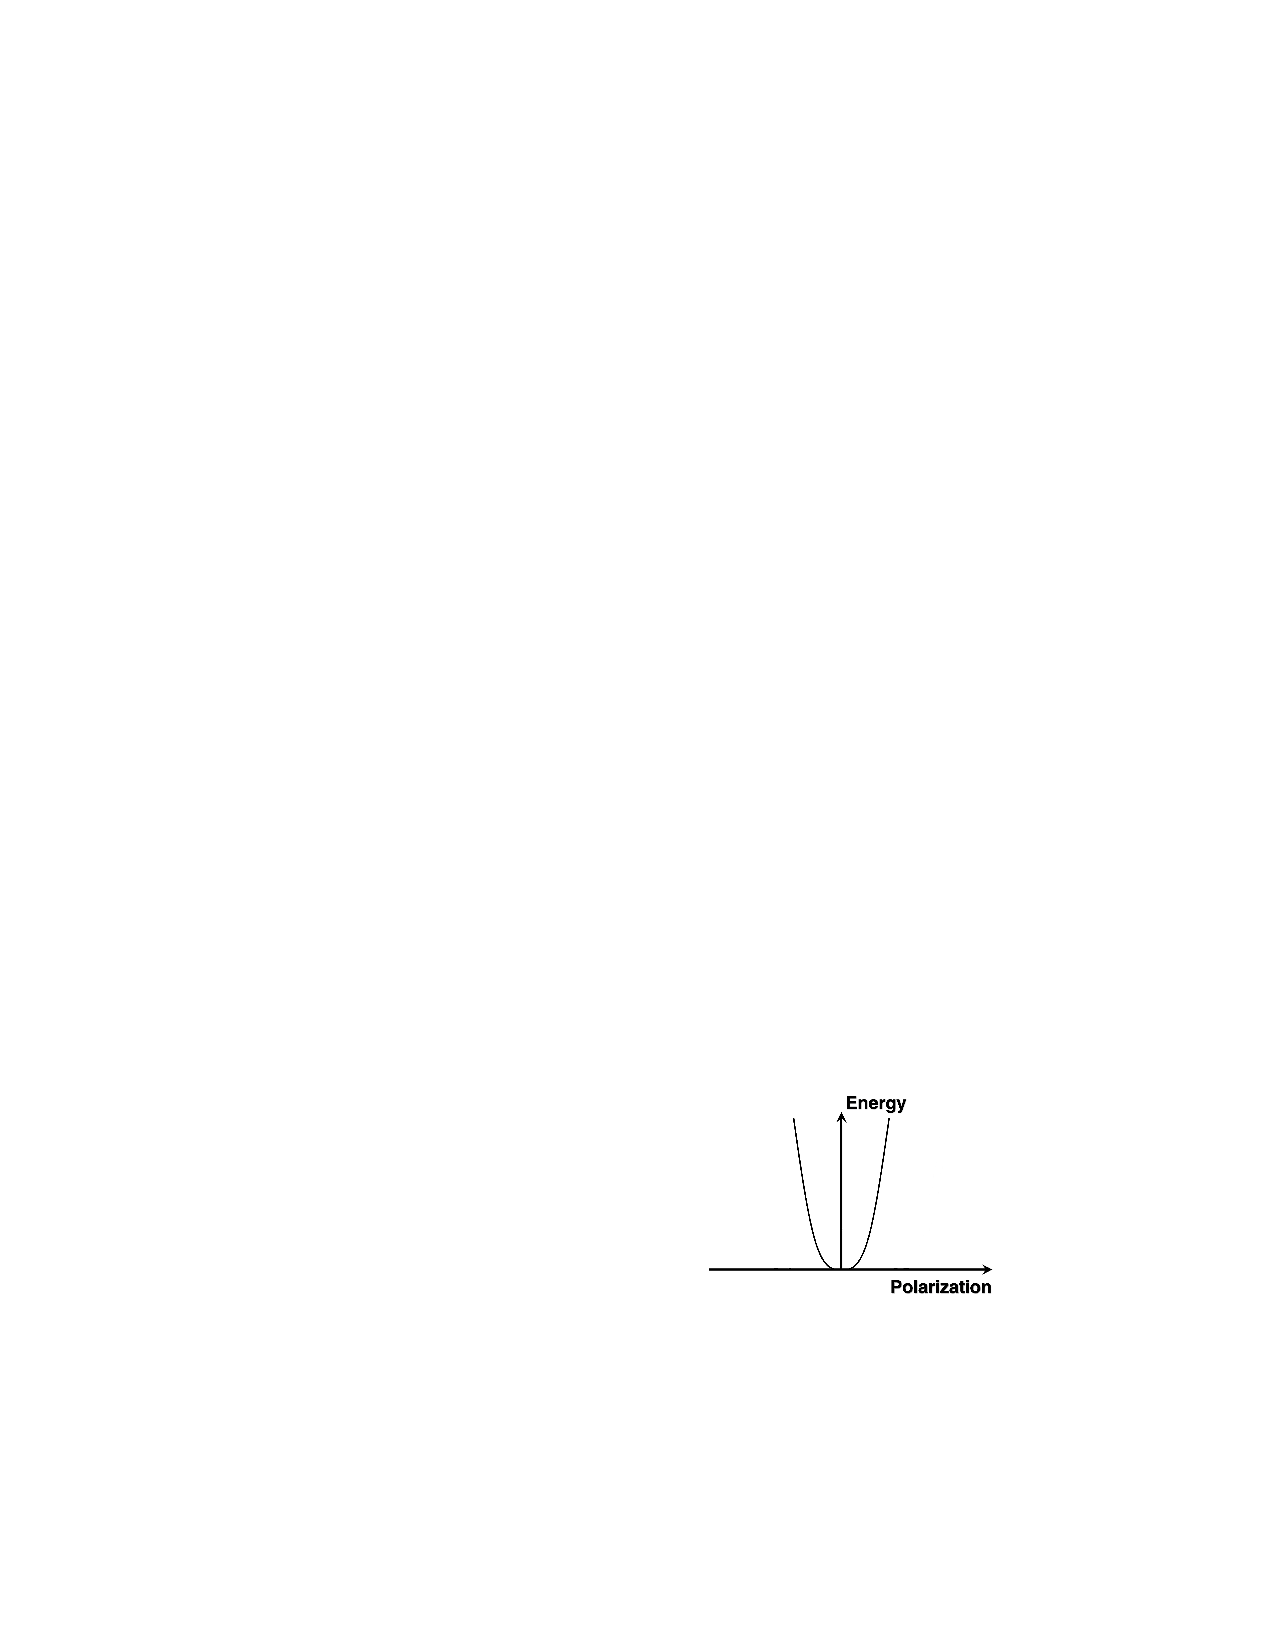
\includegraphics[width=0.45\linewidth]{./figures/materials/EvP-FE2}%
	} 	
   \subfloat[][Ferroelectric]{%
   	\label{fig:EvP-FE}%
	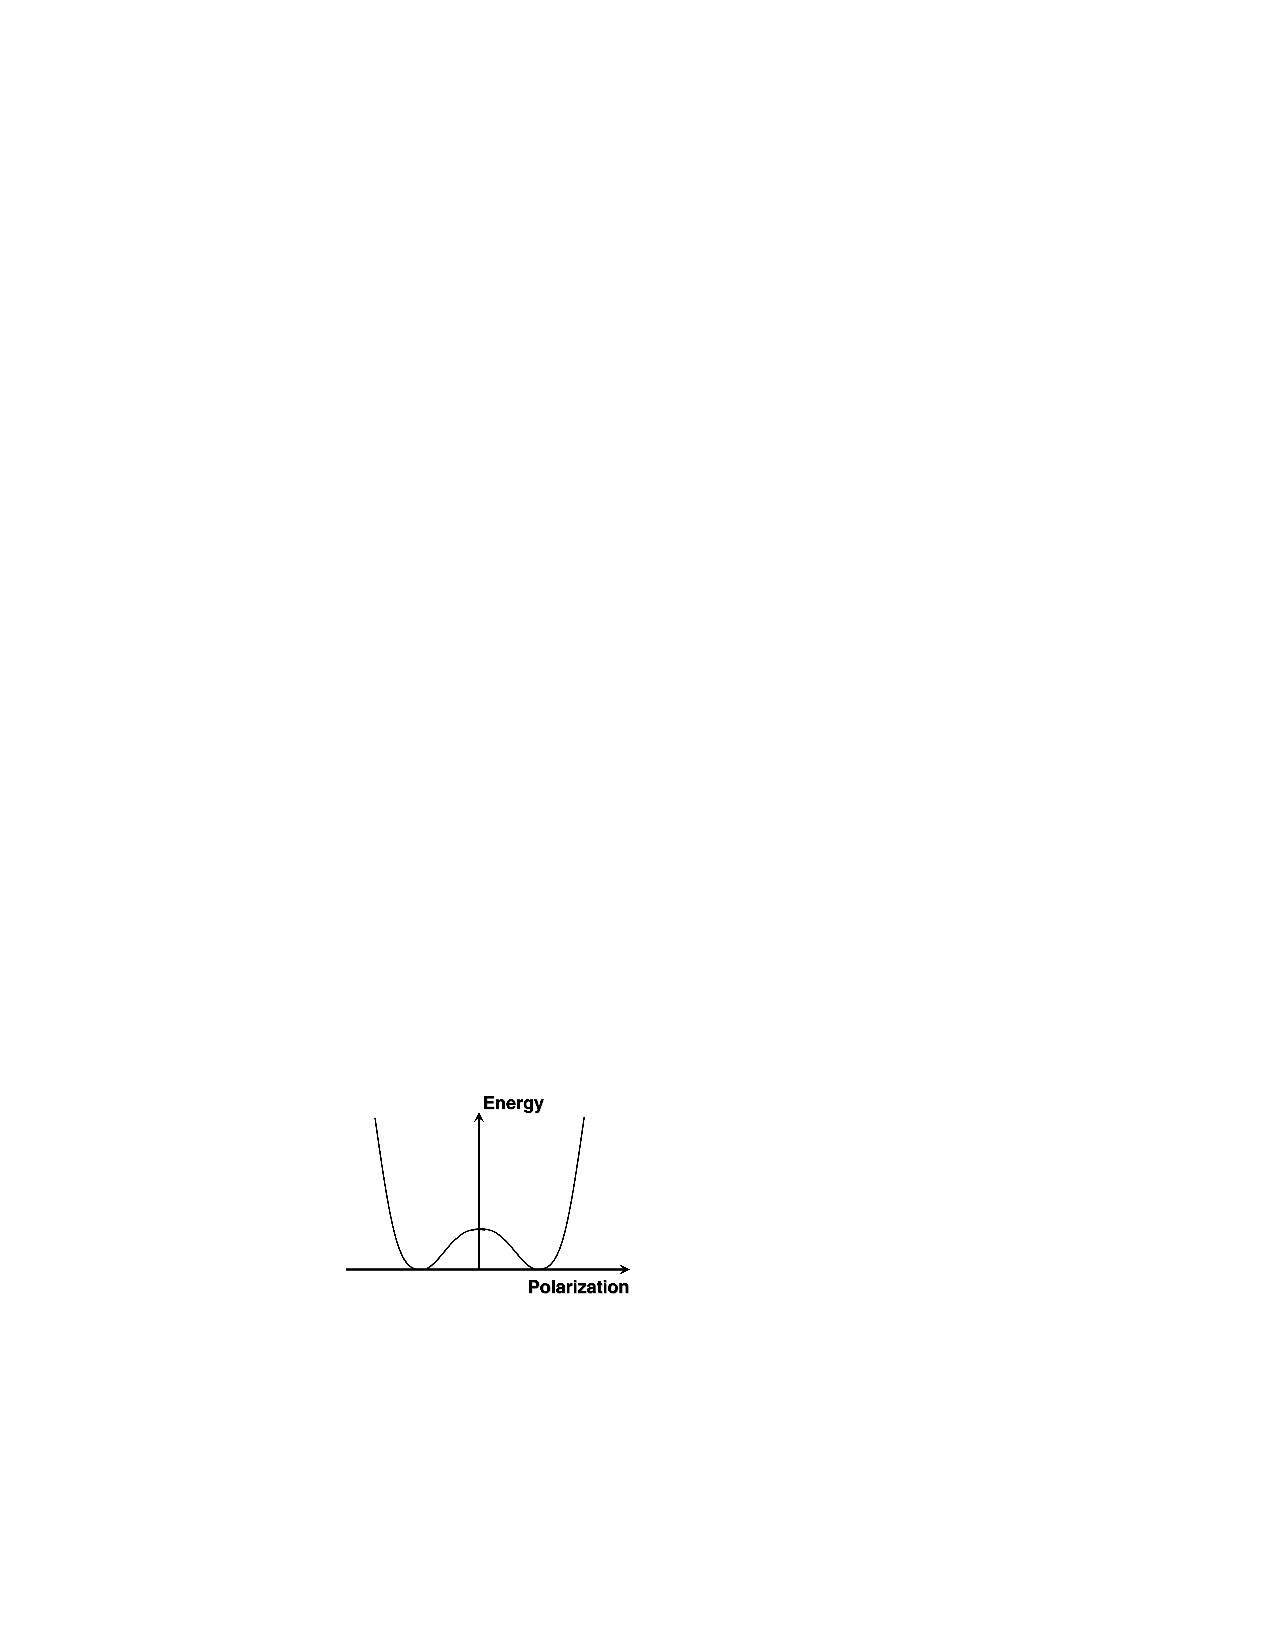
\includegraphics[width=0.45\linewidth]{./figures/materials/EvP-FE1}%
	} 	
   \caption[Energy vs. Polarization Plots for FE and PE Materials]%
   		{Example plots of the energy required to polarize a material. Ferroelectric materials (b) have %
		non-zero polarization at the energy minima. Above \Tc{} all ferroelectric materials transition %
		to a paraelectic phase (a). As temperature increases, the energy minima will approach one %
		another. }
   \label{fig:EvP}
\end{figure}

\begin{figure}[tb]
   \centering
   \subfloat[][Paraelectric]{%
   	\label{fig:PvElec-PE}%
	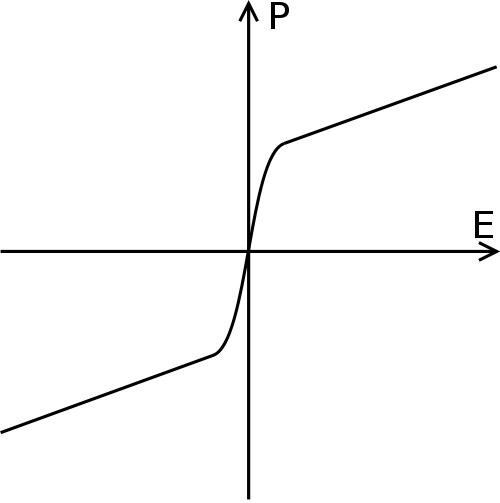
\includegraphics[width=0.4\linewidth]{./figures/materials/PvElec-PE}%
	} 
   \hspace{0.5cm}	
   \subfloat[][Ferroelectric]{%
   	\label{fig:PvElec-FE}%
	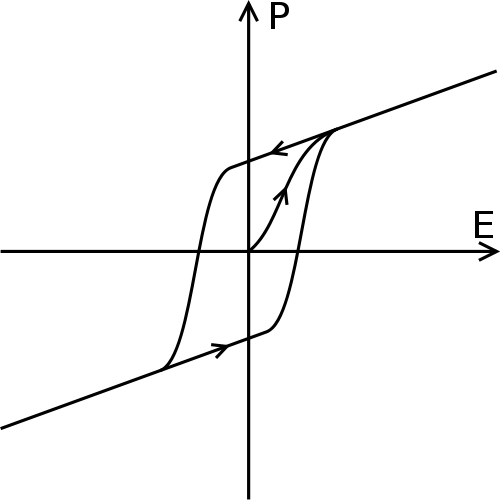
\includegraphics[width=0.4\linewidth]{./figures/materials/PvElec-FE}%
	} 	
   \caption[Polarization vs. Applied Field Plots for FE and PE Materials]%
   		{Example plots of the polarization as a function of applied field. (a) Paraelectric materials %
		have two regions of polarizability; at low E the polarization increases quickly with the field, %
		as E increases the rate of increase decreases. (b) Ferroelectric materials show similar %
		behavior, but additionally have hysteresis. This means that the films are switchable %
		between two states, but it is difficult to obtain zero polarization.}
   \label{fig:PvElec}
\end{figure}

%%%%%%%%%%%%%%%%%%%%%%%%%%%%%%%%%%%%%%%%%%%%%%%%%%%
%%%%%%%%%%%%%%%%%%%%%%%%%%%%%%%%%%%%%%%%%%%%%%%%%%%
%%%%%%%%%%%%%%%%%%%%%%%%%%%%%%%%%%%%%%%%%%%%%%%%%%%































\chapter{Synthesis Methods}
\label{chap:synthesis}
\thispagestyle{empty}

%%%%%%%%%%%%%%%%%%%%%%%%%%%%%%%%%%%%%%%%%%%%%%%%%%%
%%%%%%%%%%%%%%%%%%%%%%%%%%%%%%%%%%%%%%%%%%%%%%%%%%%
%%%%%%%%%%%%%%%%%%%%%%%%%%%%%%%%%%%%%%%%%%%%%%%%%%%

Synthesis of perovskite oxides has been demonstrated using a wide range of techniques. These range from solution-based processing methods (sol-gel approach), to physical vapor methods (molecular beam epitaxy and pulsed laser deposition), and gas phase chemical methods (chemical vapor deposition and atomic layer deposition). This review will briefly discuss sol-gel, physical vapor deposition, as well as CVD methodology, but will focus in more depth on films deposited via ALD. 

%%%%%%%%%%%%%%%%%%%%%%%%%%%%%%%%%%%%%%%%%%%%%%%%%%%
%%%%%%%%%%%%%%%%%%%%%%%%%%%%%%%%%%%%%%%%%%%%%%%%%%%
%%%%%%%%%%%%%%%%%%%%%%%%%%%%%%%%%%%%%%%%%%%%%%%%%%%

\section{Sol-Gel Processing}

\lipsum

%%%%%%%%%%%%%%%%%%%%%%%%%%%%%%%%%%%%%%%%%%%%%%%%%%%
%%%%%%%%%%%%%%%%%%%%%%%%%%%%%%%%%%%%%%%%%%%%%%%%%%%
%%%%%%%%%%%%%%%%%%%%%%%%%%%%%%%%%%%%%%%%%%%%%%%%%%%

\section{Physical Vapor Deposition}

\lipsum

%%%%%%%%%%%%%%%%%%%%%%%%%%%%%%%%%%%%%%%%%%%%%%%%%%%
%%%%%%%%%%%%%%%%%%%%%%%%%%%%%%%%%%%%%%%%%%%%%%%%%%%
%%%%%%%%%%%%%%%%%%%%%%%%%%%%%%%%%%%%%%%%%%%%%%%%%%%

\section{Metallorganic Chemical Vapor Deposition}

\lipsum

%%%%%%%%%%%%%%%%%%%%%%%%%%%%%%%%%%%%%%%%%%%%%%%%%%%
%%%%%%%%%%%%%%%%%%%%%%%%%%%%%%%%%%%%%%%%%%%%%%%%%%%
%%%%%%%%%%%%%%%%%%%%%%%%%%%%%%%%%%%%%%%%%%%%%%%%%%%

\section{Atomic Layer Deposition}
	
Atomic Layer Deposition (ALD) is a modification on standard CVD processes, with a few major differences. The defining aspect of an ALD process is the separation of the overall reaction into two steps: first the precursor is allowed to react with the substrate surface (see reaction~\ref{chem:TMA1}), excess reactant is purged from the chamber and an oxidizer is introduced to complete the reaction (see reaction~\ref{chem:TMA2}). These reactions show a very simple ALD reaction between trimethylaluminum (TMA) and water. 

\begin{reactions}
	Al(CH3)3 + M-OH_{surf} &-> M-O-Al(CH3)2_{\,surf} + CH4 \label{chem:TMA1}%
		\AddRxnDesc{TMA: Precursor-Surface Site Reaction}%
		\\
	M-O-Al(CH3)2_{\,surf} + 2H2O &-> M-O-Al(OH)2_{\,surf} + 2CH4 \label{chem:TMA2}%
		\AddRxnDesc{TMA: Ligand Oxidation \& Site Regeneration}
\end{reactions}


In this example, it is seen that the first stage allows the TMA to react with the hydrated substrate surface to form part of a layer of alumina (\ce{Al2O3}), liberating a molecule of methane as a byproduct. In the next step, the remaining ligands are stripped away from the bound TMA molecule and replacing them with hydroxy groups. This returns the system to the initial state --- where the surface is presenting sites available to react with more TMA --- and the cycle is completed. 

Having only surface reactions be permitted, as opposed to CVD where gas-phase interactions dominate, affords ALD a number of unique characteristics. One of these is the concept of the ``self-limiting'' growth mode. This behavior arises from the limited number of available reaction sites; when all of these have either been reacted with or made unavailable by a blocking mechanism such as stearic hindrance from other local chemisorbed precursor the reaction can no longer proceed. At this point, additional available precursor is not going to be utilized, and instead will be removed and treated as waste material. The system is then evacuated, and a inert purge gas such as dry nitrogen or argon (at UHP grade) is flowed through the reactor. The purge gas serves both to push any remaining gases out of the reactor as well as to help desorb physisorbed species from the surface. \reword{If these are allowed to remain adsorbed they would react with the oxidant and negate the surface-limited aspects of ALD.} The system would then again be evacuated, and the oxidant introduced and then pumped away to complete the cycle. 

In the implementation of most ALD systems, the purge gas is also used as a carrier gas for the precursors. Thus a constant flow of gas is passed through the system, instead of having it occasionally fully evacuated, and the precursor is able to be delivered from its source to the reactor more effectively. For some precursor compounds, in particular those with a low vapor pressure, having carrier-assisted transportation can greatly improve the behavior of the system. 

Because of the self-limiting behavior, each deposition cycle is limited to a theoretical maximum of one monolayer of material (in practice a much lower coverage per cycle is attained), which is far less than a unit cell. Generally per cycle growth rates range between 0.03--1.5 \AA{}, with the rate being nearly invariable during most of the deposition. This gives the second defining characteristic of ALD: very high (\AA\ level) thickness resolution. The downside of this aspect is that growths are generally much slower than other types of depositions; ALD is generally slower by an order of magnitude or more than a similar CVD process, as an example. This has proved invaluable in many processes where high precision is critical, such as electronics manufacturing. Intel, for example, uses ALD to deposit extremely thin layers of a high-$\kappa$ dielectric (such as hafnia, \ce{HfO2}) for use as the gate oxide in its transistors, with layer thickness generally less than 2 nm. 

This method will produce a layer of a binary oxide material (\ce{AO_{x}}), if more complex materials are desired the method must be changed. The basic principles remain the same; one would perform the procedure for depositing a cycle of a binary oxide and then change the precursor and deposit another cycle of a different oxide material. For example, if one wished to deposit \PTO{}, one would begin by depositing a layer of \ce{TiO2} and then depositing a layer of lead oxide (\ce{PbO}). Repeating this set of cycles --- a super-cycle --- would eventually form the \PTO{} film. 

However, deposition of complex oxides is not this simple in practice. In many cases, running each oxide cycle in a 1:1 ratio will deposit a non-stoichiometric material. This makes it necessary to modify the method to deposit more of one type of oxide than the other. For example, if a material is Ti-rich the super-cycle ratio would be modified to increase the number of lead oxide cycles as compared to the titania cycles. \reword{Needs more here.}

ALD reactions are rather sensitive to a number of factors, such as temperature. The temperature must be high enough that the reactants have sufficient energy to drive the surface reaction but not so high as to allow undesirable reactions to activate (e.g. precursor cracking or surface material desorption). Precursor selection is also very important, for similar reasons. The precursors must also be incapable of reacting with themselves, to allow the self-limiting mechanism to work properly. \reword{This section needs more work.}


%
%\begin{subreactions}
%	\label{chem:2TMA}
%	\begin{reactions}
%		Al(CH3)3 + M-OH_{surf} &-> M-O-Al(CH3)2_{\,surf} + CH4 \label{chem:2TMA1} \\
%		M-O-Al(CH3)2_{\,surf} + 2H2O &-> M-O-Al(OH)2_{\,surf} + 2CH4 \label{chem:2TMA2}
%	\end{reactions}
%\end{subreactions}
%
%\begin{subreactions}
%\newcommand*{\thesubequation}{(\reactiontag.\alph{equation})}
%\label{chem:TMA}
%\begin{align}
%	\cee{Al(CH3)3 + M-OH_{surface} &-> M-O-Al(CH3)2_{\ surf} + CH4}%
%		\label{chem:TMA1}
%		\\
%	\cee{M-O-Al(CH3)2_{\ surf} + 2H2O &-> M-O-Al(OH)2_{\ surf} + 2CH4}%
%		\label{chem:TMA2}
%\end{align}
%\end{subreactions}



\lipsum








\chapter{Characterization Methods}
\label{chap:Charact}
\thispagestyle{empty}

%%%%%%%%%%%%%%%%%%%%%%%%%%%%%%%%%%%%%%%%%%%%%%%%%%%
%%%%%%%%%%%%%%%%%%%%%%%%%%%%%%%%%%%%%%%%%%%%%%%%%%%
%%%%%%%%%%%%%%%%%%%%%%%%%%%%%%%%%%%%%%%%%%%%%%%%%%%
%
%\section{Imaging Techniques}
%
%A variety of imaging methods were used to visually inspect the samples at a variety of length scales. The two main techniques that proved invaluable for this aspect of the project were scanning electron microscopy (SEM) as well as atomic force microscopy (AFM). 
%
%%%%%%%%
%
%\subsection{Scanning Electron Microscopy}
%
%Scanning electron microscopy is a widely used technique for imaging nanostructures. 
%
%\lipsum
%
%
%%%%%%%%
%
%\subsection{Atomic Force Microscopy}
%
%\lipsum
%
%%%%%%%%%%%%%%%%%%%%%%%%%%%%%%%%%%%%%%%%%%%%%%%%%%%
%%%%%%%%%%%%%%%%%%%%%%%%%%%%%%%%%%%%%%%%%%%%%%%%%%%
%%%%%%%%%%%%%%%%%%%%%%%%%%%%%%%%%%%%%%%%%%%%%%%%%%%

\section{Compositional Analysis}
\label{sec:Charact-Comp}

%%%%%%%

\subsection{Energy-Dispersive X-Ray Spectroscopy}

Energy dispersive X-ray spectroscopy (EDXS) is a commonly used analysis technique for determining the composition of a sample. In this process, a sample is bombarded with high-energy electrons (2--30 keV) which interact with the sample. Some of these electrons will cause a core electron of an atom in the sample to be ejected. This leaves a vacant orbital in the inner shell, which a higher energy electron will fill. In the process of filling the vacancy, the electron will emit an X-ray photon equal to the energy difference between the two states. These energies are referred to using the common X-ray spectroscopy nomenclature (e.g. K$_{\alpha}$, K$_{\beta}$, L$_{\alpha}$). An illustration of this process can be found in figure~\vref{fig:EDXS-image}.  

Since the energies of the emitted photons are very specific to each element, the procedure can be used to identify the presence of the element in the sample. With some calibration, EDXS can also be used to quantify the relative amounts of each element in a sample using the different number of collected photons. However, this can sometimes be difficult due to some elements have overlapping spectrums as the peaks are not sharp and different elements can have similar energies for some transitions. 

One of the downsides of EDXS is that the interaction volume of electrons is much larger deeper into the sample, so the surface sensitivity of the technique is smaller than with some other techniques. 

\begin{figure}[tb]
   \centering
   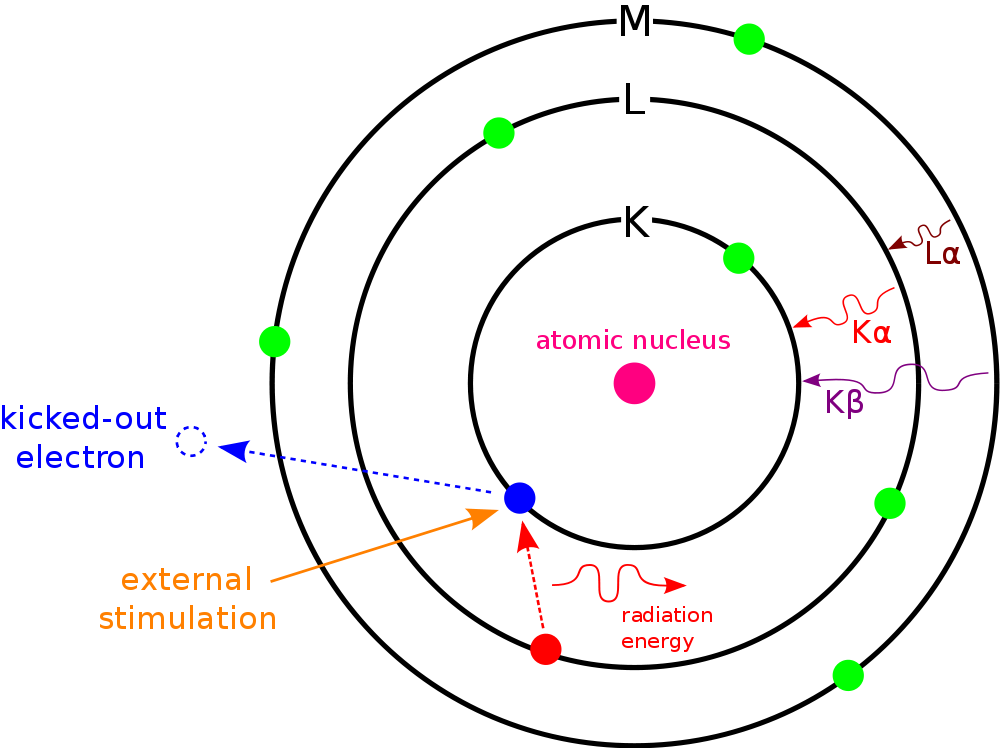
\includegraphics[width=0.66\linewidth]{./figures/characterization/EDXS-scheme} 
   \caption[Illustration of EDXS principle]%
   		{Graphic illustrating the basic mechanism for EDXS, along with the commonly used %
		notation for the various energies. The external stimulation would be a high energy %
		electron.}
   \label{fig:EDXS-image}
\end{figure}



%%%%%%%

\subsection{X-Ray Fluorescence Spectroscopy}

X-ray fluorescence spectroscopy (XRFS) is a similar technique to EDXS. In XRFS the excitation used is X-ray photons (often from a Cu K$_{\alpha}$ source with $\lambda = 1.54$ \AA), as opposed to energetic electrons. In other considerations the techniques are equivalent. 

XRFS often has a lower noise floor than EDXS, allowing smaller signals to be more easily identified (such as in ultra-thin films). It does suffer the same disadvantage of having overlapping peaks. This resolution issue can be alleviated to some degree by using wavelength dispersive XRFS (WD-XRFS), which uses diffraction techniques to analyze the emitted x-ray spectrum. 

%%%%%%%

\subsection{Rutherford Backscattering Spectroscopy}




%%%%%%%%%%%%%%%%%%%%%%%%%%%%%%%%%%%%%%%%%%%%%%%%%%%
%%%%%%%%%%%%%%%%%%%%%%%%%%%%%%%%%%%%%%%%%%%%%%%%%%%
%%%%%%%%%%%%%%%%%%%%%%%%%%%%%%%%%%%%%%%%%%%%%%%%%%%

\section{Thin Film Characterization}
\label{sec:Charact-ThinFilm}


%%%%%%%
	
\subsection{Variable Angle Spectroscopic Ellipsometry}

Ellipsometry is a powerful non-destructive optical technique that allows for the determination of a large number of properties of complex thin film structures. The basic tenet of ellipsometry relies on the analysis of the change in polarization state of a reflected light beam after interaction with the sample. The incident beam is generally linearly polarized, but upon reflection becomes elliptically polarized due to a phase shift in the components of the beam in the s- and p-plane, as well as a change in their relative amplitudes. The phase shift is correlated to the ellipsometric parameter $\Delta$, while the amplitude change is given by $\tan\Psi$ ($\Psi$ is the angle between the s-plane and the major axis of the ellipse). The last major parameter is the incident angle, denoted by $\Phi$. A schematic diagram illustrating these parameters can be seen in figure~\vref{fig:ellipsometry}. 

\begin{figure}[tb]
   \centering
   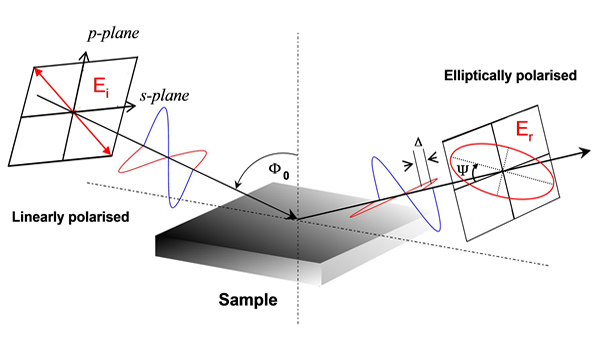
\includegraphics[width=\linewidth]{./figures/characterization/ellipsometryDiagram_simple} 
   \caption[Ellipsometric Beam Path and Modeling Parameters]{Schematic of the beam path during an %
   					ellipsometric measurement, \\ critical parameters are indicated}
   \label{fig:ellipsometry}
\end{figure}

From these parameters, one can directly determine the ratio between the reflectance in the p-plane ($r_{p}$) and the reflectance in the s-plane ($r_{s}$) from the fundamental ellipsometric relation (eqn.~\vref{eq:ellipsometry}).  Once this relationship is known, the Fresnel equations (eqn.~\vref{eq:fresnel}) can be used to numerically determine the value of the complex index of refraction at the specific wavelength of the incoming beam. The complex index of refraction (eqn.~\vref{eq:complexindex}) describes the nominal index of refraction but additionally includes an imaginary term to describe absorption of light in the material (commonly referred to as the extinction coefficient, $\kappa$).  

\begin{equation}
 \label{eq:ellipsometry}
 \displaystyle
	\rho = \frac{r_{p}}{r_{s}} = \tan(\Psi)e^{i\Delta}
\end{equation}

\begin{subequations}
\label{eq:fresnel}
\begin{align}
	r_{p} &= \frac{\tilde{n}_{1}\sqrt{1- \left(\frac{\tilde{n}_{1}}{\tilde{n}_{2}}\sin\Phi\right)} - \tilde{n}_{2}%
			\cos\Phi}{\tilde{n}_{1}\sqrt{1- \left(\frac{\tilde{n}_{1}}{\tilde{n}_{2}}\sin\Phi\right)} + %
			\tilde{n}_{2}\cos\Phi} \\
        	r_{s} &= \frac{\tilde{n}_{1}\cos\Phi - \tilde{n}_{2}\sqrt{1- \left(\frac{\tilde{n}_{1}}{n_{2}}\sin\Phi\right)}}%
			{\tilde{n}_{1}\cos\Phi + \tilde{n}_{2}\sqrt{1- \left(\frac{\tilde{n}_{1}}{\tilde{n}_{2}}\sin\Phi\right)}}
\end{align}
\end{subequations}

\begin{equation}
 \label{eq:complexindex}
 \displaystyle
	\tilde{n} = n + i\kappa
\end{equation}

This type of analysis is sufficient for thick, isotropic samples without any surface layers (e.g. surface oxides or adsorbed gases), and can directly provide the value of $\tilde{n}$. However, once layers are stacked upon one another, the system becomes very difficult to analyze directly due to interference effects between the layers. It becomes necessary to use modeling techniques to determine the correct values of $\tilde{n}$ and thickness ($t$) for each layer. 

The power of ellipsometry as a high-resolution optical analysis technique stems from the use of phase and polarization changes. This allows the analysis to overcome the diffraction limit, and can be accurate down to angstroms. Properly modeling the system is critical for this analysis to be as precise as possible. Thus, there have been refinements of the ellipsometric method to greatly increase the amount of experimental data points, allowing the overall system to be over-determined and thus letting all of the systems parameters to be calculated. 
	
Variable angle spectroscopic ellipsometry (VASE) is one of these variants. Spectroscopic ellipsometry differs from single-wavelength ellipsometry by utilizing a broad-band light source as opposed to a monochromatic source. By performing ellipsometric analysis at each of the wavelengths, one can determine the wavelength (and thus photon-energy) dependence of $n$ and $\kappa$. This not only helps to improve data analysis (as it can generally be safely assumed that the values of $n$ and $\kappa$ are smooth functions of $\lambda$), but allows for the determination of many other properties of the material. Of specific importance is the complex dielectric function ($\tilde{\epsilon}$), which is related to $\tilde{n}$ by the relation shown in equation~\vref{eq:dielectricfunction}. Knowing these functions can allow for determination of electronic properties such as the bandgap energy, the absorption coefficient, amongst others. Finally, by obtaining spectra at a number of different incident angles, one directly provides additional data points across the entire wavelength spectrum. Even a small number of additional angles can quickly provide sufficient data points for the system to be over determined. 

\begin{equation}
 \label{eq:dielectricfunction}
 \displaystyle
	\tilde{\epsilon} = \epsilon_{1} + i\epsilon_{2} = \tilde{n}^{2}
\end{equation}

During this project, a VASE M-2000U system (figure~\vref{fig:M2000_image}) built by J.A. Woollam, inc. was used to collect all of the ellipsometric data. In addition, data analysis was performed using the WVASE32{$^{\copyright}$} package also provided by J.A. Woollam, inc. The system utilizes a rotating compensator and a CCD detector to greatly decrease data collection time by collecting data across the entire spectrum simultaneously.  More information on this system is available from the J.A. Woollam, inc. webpage.\cite{woollam-web}

\begin{figure}[tb]
   \centering
   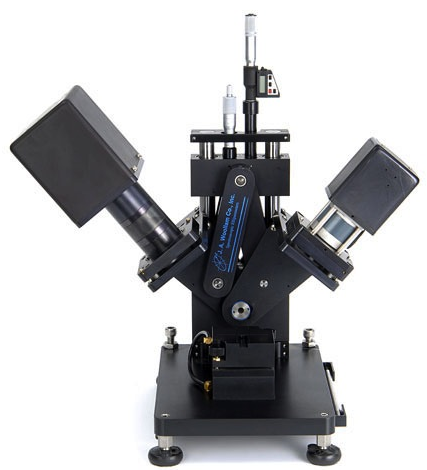
\includegraphics[width=0.5\linewidth]{./figures/characterization/M2000_ellipsometer_image.png} 
   \caption[J.A. Woollam M-2000U Ellipsometer]%
   		{Photograph of the J.A. Woollam M-2000U variable \\%
   		 angle spectroscopic ellipsometer (VASE)}
   \label{fig:M2000_image}
\end{figure}


%%%%%%%%%%%%%%%%%%%%%%%%%%%%%%%%%%%%%%%%%%%%%%%%%%%
%%%%%%%%%%%%%%%%%%%%%%%%%%%%%%%%%%%%%%%%%%%%%%%%%%%
%%%%%%%%%%%%%%%%%%%%%%%%%%%%%%%%%%%%%%%%%%%%%%%%%%%
	
\section{Phase Identification}
\label{sec:Charact-PhaseID}

%%%%%%%

\subsection{X-Ray Diffraction}

\lipsum	

%%%%%%%

\subsection{Grazing Incidence X-Ray Diffraction}

\lipsum

%%%%%%%%%%%%%%%%%%%%%%%%%%%%%%%%%%%%%%%%%%%%%%%%%%%
%%%%%%%%%%%%%%%%%%%%%%%%%%%%%%%%%%%%%%%%%%%%%%%%%%%
%%%%%%%%%%%%%%%%%%%%%%%%%%%%%%%%%%%%%%%%%%%%%%%%%%%

\section{Thermal Analysis}
\label{sec:Charact-Thermal}

%%%%%%%

\subsection{Thermogravimetric Analysis}

Thermogravimetric analysis (TGA) is a very useful tool when attempting to determine the viability of a precursor in an ALD process. It allows for estimation of vaporization rate at various temperature rates as well as indications of chemical breakdown (i.e. thermalization) which would negate the precursor's usefulness. 

At its core, TGA is a measurement of mass loss as a function of temperature or time. A small sample (1--10 mg) of material is placed in a microgram balance pan and suspended inside a furnace. The furnace is then heated at a specified rate while the sample mass is carefully monitored. For the experiments used in this study (evaluation of thermal vaporization and thermal degradation) it is important to ensure that the testing environment is inert. This is accomplished by using a platinum pan in the microgram balance and constantly purging the furnace with a small flow of dry nitrogen gas. The heating rate can be varied according to a pre-determined program to provide more information at various individual temperatures. 

This technique was used to evaluate various precursor candidates for the lead oxide half of the \PTO deposition procedure. The instrument used was a Q50 TGA device (fig.~\vref{fig:Q50-image}).  A detailed discussion of TGA procedures and the investigated chemicals can be found in subsequent chapters (see~\vref{sec:Methods-TGA} and \vref{chap:Results-Thermal}). 

\begin{figure}[tb]
   \centering
   \subfloat[Q50 TGA][Q50 TGA]{%
   	\label{fig:Q50-image}%
	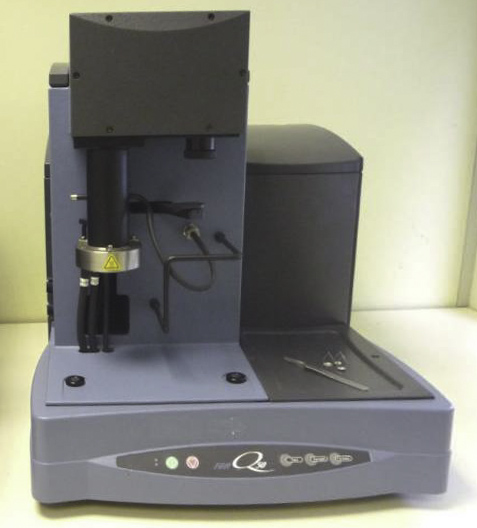
\includegraphics[width=0.45\linewidth]{./figures/characterization/Q50-TGA}%
	} 
  \subfloat[Q2000 DSC][Q2000 DSC]{%
   	\label{fig:Q2000-image}%
	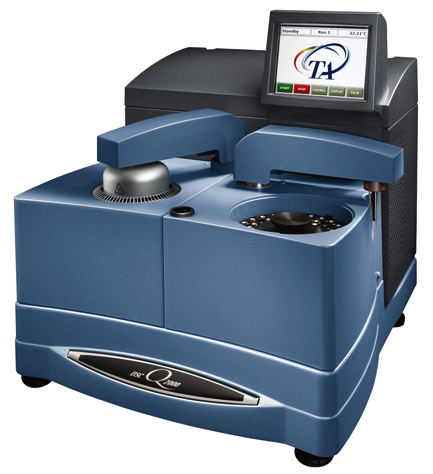
\includegraphics[width=0.45\linewidth]{./figures/characterization/Q2000-DSC}%
	} 	
   \caption[T.A. Instruments, inc. Instrumentation]%
   		{Photograph of the thermal analysis instrumentation used during this study, \\
		made by T.A.  Instruments, inc.}
   \label{fig:TA-Instruments}
\end{figure}

%%%%%%%

\subsection{Differential Scanning Calorimetry}
	
Differential scanning calorimetry (DSC) is a technique that allows for the determination of various critical temperatures for a material, and also can highlight changes in chemical structure due to degradation or other thermal processes. 

DSC is the analysis of energy absorption as a function of temperature, which is the essence of calorimetry. DSC uses a sample and reference system to isolate the energy absorbed by the sample from that of the holder pan. Sample sizes usually range from 0.3--2 mg of material; as the samples used in this study are volatile the sample pans are hermetically sealed to prevent mass loss. The sample and reference pans are then placed inside a thermally insulated chamber. The temperature of each is carefully monitored, and differing amounts of heat are applied to negate the temperature difference between the sample and reference. The difference in absorbed heat as a function of temperature is then given as the result. In general, experiments include both heating and cooling curves to gain a complete understanding of the different energies. 
	
DSC was used to analyze the behavior of precursor chemicals around their evaporation and reaction temperatures. The main goal was to determine if the material underwent any thermally-activated degradation processes at either of these two temperature ranges. At the evaporation temperature, the sample was generally cycled multiple times to simulate actual use in the ALD. These measurements were taken using a Q2000 DSC system (fig.~\vref{fig:Q2000-image}) made by T.A. Instruments, inc.	
	

































	
	
	
\chapter{Thin Film Growth}
\label{ch:SampFab}
\thispagestyle{empty}


%%%%%%%%%%%%%%%%%%%%%%%%%%%%%%%%%%%%%%%%%%%%%%%%%%%%%%%%%%
%%%%%%%%%%%%%%%%%%%%%%%%%%%%%%%%%%%%%%%%%%%%%%%%%%%%%%%%%%
%%%%%%%%%%%%%%%%%%%%%%%%%%%%%%%%%%%%%%%%%%%%%%%%%%%%%%%%%%

\section{Precursor Selection}
\label{sec:SampFab-Precursors}

\lipsum

%%%%%%%%%%%%%%%
\subsection{Titanium Source}

The source of titanium that was used was titanium(IV) isopropoxide (\TiOiPr{}, \ce{Ti(OCH(CH3)2)4}). This compound is very commonly used in ALD literature.\reword{[Citation needed]} It is a liquid precursor with a high vapor pressure and reacts easily with most oxidizers; the most commonly used oxidant for this reaction is water vapor, similar to the TMA-\ce{H2O} reaction (see section~\vref{sec:Synth-ALD}). 

%%%%%%%%%%%%%%%
\subsection{Lead Source}

Lead sources included bis(2,2,6,6-tetramethyl-3,5-heptanedionato)lead(II) (\ce{Pb(TMHD)2}) and lead(II) hexafluoroacetylacetonate (\ce{Pb(HFAc)2}). Both compounds had been referenced in literature \reword{[citation needed]}, were available from multiple chemical suppliers, and were expected to have the highest vapor pressure of the choices available at the time. 

Samples of both of these compounds were obtained from Strem Chemical, inc. \reword{(sp?)} Analysis of the precursors included thermal tests (TGA and DSC, see section~\vref{chap:Results-Thermal}) as well as test depositions of ALD films. The precursor chosen for use after testing was \TMHD{}, and films discussed further solely utilized this compound. 

%%%%%%%%%%%%%%%
\subsection{Oxidizer}

Three potential oxidants were considered; these included water, oxygen, and an ozone/oxygen mix. The choice of oxidant depends heavily on the reactivity with the potential precursors. 

The choice of titanium(IV) isopropoxide as the titanium source allows for any of the three selected oxidizers to be used. A hydrolysis reaction will occur when exposed to water vapor; in the case of oxygen or ozone the ligands will be consumed via a combustion reaction. 

The two lead precursors do not undergo hydrolysis when exposed to water, and as such require the use of the combustion pathway. In addition, it was found that the reaction proceeded more completely when the \ce{O3}/\ce{O2} mixture was used. For simplicity of the process, the \ce{O3}/\ce{O2} mix was used for both half-reactions. 

%%%%%%%%%%%%%%%%%%%%%%%%%%%%%%%%%%%%%%%%%%%%%%%%%%%%%%%%%%
%%%%%%%%%%%%%%%%%%%%%%%%%%%%%%%%%%%%%%%%%%%%%%%%%%%%%%%%%%
%%%%%%%%%%%%%%%%%%%%%%%%%%%%%%%%%%%%%%%%%%%%%%%%%%%%%%%%%%

\section{Substrate Preparation}
\label{sec:SampFab-Substrates}

Fabrication and preparation of substrates was an important part of the deposition process. Some substrates were purchased and simply cleaned, others needed to be fabricated or otherwise processed prior to cleaning and use in deposition. Three main types of substrates were used: thermally oxidized single-crystalline silicon (100) wafers, silicon wafers that had a thin layer of platinum deposited on the surface, and strontium titanate (100) single crystal substrates. 

%%%%%%%%%%%%%%%
\subsection{Si(100)} \label{sec:Si}

The silicon substrates were prepared in a simple manner. 4'' diameter silicon wafers with 200 nm of thermally grown oxide were diced into 1.5 cm x 1.5 cm pieces. When a sample was to be used for deposition, it was cleaned by one minute of sonication in acetone, followed by isopropanol, with a subsequent 5 minutes of sonication in deionized (DI) water. These were then air dried with dry nitrogen. Finally, the substrates were cleaned in a oxygen plasma cleaning system to remove any remaining organic residues present on the surface. 


%%%%%%%%%%%%%%%

\subsection{Platinized Si(100)}

Platinized silicon substrates were prepared in a similar manner to the Si(100) samples. For the initial platinization, a large piece (5 x 5 cm$^{2}$) of silicon wafer with a thin layer of native oxide, as opposed to the 200 nm of thermally grown oxide, was prepared in the manner described above. Then a 15 nm layer of platinum was deposited via ALD (deposition recipe can be found in \reword{redacted}). The substrates were then cleaved into smaller pieces for later use. 

If the samples are stored, it is recommended to again clean the samples in the standard procedure prior to use (see \vref{sec:Si}).

%%%%%%%%%%%%%%%

\subsection{STO(100) and Nb:STO(100)}

Oxide crystal substrates were prepared in such a fashion as to promote the formation of atomically flat terraces. This has the advantage of promoting a uniform surface species across the entire sample --- the etchant used in this process leaves the sample titania-terminated. 

To prepare these samples, the substrates are first pre-cleaned in a three step sonication process. The samples were cleaned for five minutes in each of acetone, methanol, and isopropyl alcohol. Subsequently, the samples were sonicated for fifteen minutes in DI water. \reword{Need to find reference and exact timings. Email Eric.}. The substrates were then dipped into buffered hydrofluoric acid to etch for \reword{35 seconds}, then removed and flushed with copious DI water.  Once the sample is thoroughly rinsed, the samples are dried using dry nitrogen. 

After the etching process, the samples are annealed at 1050\degC{} for \reword{two hours}. Once the samples are cooled, they are ready for immediate use. AFM can be used to confirm the presence of atomic terraces. 

If the samples are stored, it is recommended to again clean the samples in the standard procedure (see \vref{sec:Si}).

%%%%%%%%%%%%%%%%%%%%%%%%%%%%%%%%%%%%%%%%%%%%%%%%%%%%%%%%%%
%%%%%%%%%%%%%%%%%%%%%%%%%%%%%%%%%%%%%%%%%%%%%%%%%%%%%%%%%%
%%%%%%%%%%%%%%%%%%%%%%%%%%%%%%%%%%%%%%%%%%%%%%%%%%%%%%%%%%

\section{Deposition Parameters}
\label{sec:SampFab-DepParams}

There are four main parameters that can affect the behavior of an ALD deposition.  These are the growth temperature, the dosage of each precursor, the purge time between doses, and any extended precursor-surface exposure time. 

%%%%%%%%%%%%%%%

\subsection{Growth Temperature}

The temperature of the growth chamber has a strong effect on reaction behavior. ALD reactions are sensitive to temperature, and will only proceed properly within a certain range known as the `ALD window.' Outside of this range, the reaction enters one of a number of different regimes; these are determined by comparing the growth rate of the deposition to that of a reaction in the self-limiting saturated ``ALD mode.'' 

If the growth temperature is less than the lower bound of the ALD window, the two regimes are condensation limited and activation energy limited. Condensation limited growth occurs when the substrate temperature is low enough that precursor condenses onto the surface without reacting with the presented sites. This causes higher than expected growth rates, and a lack of self-limiting behavior. If the reaction instead proceeds into the activation energy limited regime, molecules of precursor lack sufficient energy to react with the surface. This is characterized by lower deposition rates. 

Conversely, if the reactor temperature is excessive the reaction again become anomalous. Decomposition limited growth, characterized by excessive deposition, is a result of thermal cracking of the precursor materials. This reaction is not limited to the surface, and accounts for the extra material being deposited. Lower deposition rates indicate that the temperature is sufficient to cause desorption of previously-reacted material from the sample. 

For an ALD run to be successful, the acceptable temperature window for all of the reactions should overlap in some temperature range. This can become difficult with reactions requiring multiple metal precursors (e.g. \PTO, a combination of \ce{TiO2} and \ce{PbO}), as these can have widely varying ALD windows for their respective reactions. 

%%%%%%%%%%%%%%%

\subsection{Precursor Dosage}

The dosage of precursor or oxidant to the surface is another parameter of critical importance. An ALD reaction requires a minimal amount of precursor to sufficiently saturate the surface, while it is beneficial to minimize any excess precursor as it will be a wasted byproduct (minimizing costs, environmental impact, etc.). 

The vaporization behavior of the precursor can have a dramatic impact on how simple or difficult it is to deliver a saturating dose to the surface. Some materials have readily available precursors with high vapor pressures; titanium isopropoxide and trimethylaluminum (TMA) are both liquids, and tetrakis(dimethylamido)hafnium (\ce{Hf\{N(CH3)2\}4}) is a low-melting temperature solid. These are commonly used precursors for depositing their respective oxides. This vapor pressure becomes an important consideration when choosing a potential compound for use in ALD (as discussed in section~\vref{sec:SampFab-Precursors}).

Insufficient dosing is apparent in a deposition run by a slower than average growth rate, or also as a non-uniform deposition rate across the sample. However, overdosing is not readily apparent in an ALD-mode deposition. The dose must be lowered to a point where the dose is insufficient, and then increased back to a saturating level. 

Controlling the dose is dependent on injection time (which is the time the valve between the process line and the precursor storage vessel is open), precursor temperature, and the cycle duration (time between precursor injections). By increasing either the injection time or the precursor's temperature the dose is increased, except in some cases with low vapor pressure materials. In this case, it can sometimes be found that the evaporation kinetics are slow and it takes additional time to build up a sufficient amount of vapor to provide a dose to the reactor. 

If necessary, multiple doses of precursor can be delivered to the sample during each cycle to increase the total delivered dose.

%%%%%%%%%%%%%%%

\subsection{Purge Time}

Purge time is important as it gives time for the \ce{N2} flow to flush any remaining byproducts and excess reactants from the reactor zone. It also allows time between cycles which allows for low vapor pressure precursors to regenerate evaporated material; if this time is too short to fully regenerate the dose in the cylinder the precursor will eventually appear to be depleted during the course of the deposition. 

%%%%%%%%%%%%%%%

\subsection{Exposure Time}

Exposure time denotes the time where the precursor is held in the reaction zone to increase the amount of time during which the surface reaction can occur. This is beneficial for two types of depositions. In the case of low-reactivity precursors, it increases the amount of time that the precursor is available to the surface, greatly increasing the surface coverage per cycle. Exposure mode is also beneficial for depositing upon three dimensional structures, especially those with a high aspect ratio, e.g. nanotube templates. This extra dwell time of the precursor allows for diffusion of reactant into the structure, for a uniform coverage upon the entirety of the surface. Purge time must be increased accordingly to allow for byproducts to diffuse back out of the structure. 

%%%%%%%%%%%%%%%%%%%%%%%%%%%%%%%%%%%%%%%%%%%%%%%%%%%%%%%%%%
%%%%%%%%%%%%%%%%%%%%%%%%%%%%%%%%%%%%%%%%%%%%%%%%%%%%%%%%%%
%%%%%%%%%%%%%%%%%%%%%%%%%%%%%%%%%%%%%%%%%%%%%%%%%%%%%%%%%%

\section{Post-Deposition Annealing}
\label{sec:SampFab-Annealing}

Two types of annealing procedures were used in this study. Oven annealing, with the simple use of a furnace in ambient atmosphere; and rapid thermal annealing (RTA), characterized by very high heating and cooling rates and performed in an inert atmosphere (dry \ce{N2}). 


%%%%%%%%%%%%%%%

\subsection{Oven Annealing}

In oven annealing, the samples to be processed are placed in a cold oven in the ambient atmosphere of the laboratory. The samples are then heated gradually at a rate of 10--25\degC{} per minute up to the final annealing temperature, which ranged from 600--900\degC{}. The samples are then allowed to heat-treat for 120 minutes at the process temperature, and then the furnace is allowed to return to room temperature. 

This conventional heating pattern allows the sample to obtain its equilibrium crystalline phase composition, be that a single crystalline phase, polycrystalline, or involve multiple phases or materials. This was the annealing method most commonly used during this study. 

%%%%%%%%%%%%%%%

\subsection{Rapid Thermal Annealing}

Rapid thermal annealing (RTA), as its name suggests, involves very high heating and cooling rates. RTA systems can heat at rates over 10\degC{} per second, allowing the chamber and sample to reach the process temperature very quickly. Similarly, processing times are generally much shorter, and are generally no longer than 10--15 minutes. Cooling, facilitated by a water cooling apparatus, also occurs rapidly. These sharp gradients can have different effects on the crystal structure of the film, locking in different phases in the material that may otherwise dissociate given more time during heating or cooling. 

In this study samples processed via RTA used a \reword{HeatPulse XXXX?} RTA system (see fig.~\reword{XX}), which allowed for automatic control of the process. Sample processing conditions can be found in table~\vref{tbl:LoSamples} in the appendix. 






\chapter{Analysis Methods}
\label{ch:Methods}
\thispagestyle{empty}


%%%%%%%%%%%%%%%%%%%%%%%%%%%%%%%%%%%%%%%%%%%%%%%%%%%%
%%%%%%%%%%%%%%%%%%%%%%%%%%%%%%%%%%%%%%%%%%%%%%%%%%%%
%%%%%%%%%%%%%%%%%%%%%%%%%%%%%%%%%%%%%%%%%%%%%%%%%%%%

\section{Thermal Analysis}
\label{sec:Methods-Thermal}

%%%%%%%%%%%%%%%%

\subsection{Thermogravimetric Analysis}

Collection of TGA data was straightforward, and performed as described in the manual for the Q50 TGA. After initial calibration of the system, a small sample (5--10 mg) of material was placed into a platinum sample pan. The pan was then loaded into the furnace of the TGA and a small flow of purge gas (\ce{N2} at 50 mL/min) was started to isolate the sample from ambient atmosphere. At this point the desired test sequence was programmed into the controller and the instrument allowed to begin data collection. 

%%%%%%%%%%%%%%%%

\subsection{Differential Scanning Calorimetry}

DSC experiments were performed in a similar method as those of TGA. Small samples of material (3--5 mg) were loaded into hermetically sealed sample pans inside of a glovebox containing an inert atmosphere. The use of hermetically sealed pans was important as the material was intended to vaporize, and the loss of material through escaped vapor would change the results of the test. In addition, loading the material in inert atmosphere prevents the presence of oxidants within the sample atmosphere during the test. An additional sample pan was sealed with no contents to act as a reference. Both pans were weighed precisely on a high-resolution balance and then loaded into the sample chamber of the Q2000. Again, the desired testing sequence was programmed into the instrument's controller, and the experiment was run automatically. 

%%%%%%%%%%%%%%%%%%%%%%%%%%%%%%%%%%%%%%%%%%%%%%%%%%%%
%%%%%%%%%%%%%%%%%%%%%%%%%%%%%%%%%%%%%%%%%%%%%%%%%%%%
%%%%%%%%%%%%%%%%%%%%%%%%%%%%%%%%%%%%%%%%%%%%%%%%%%%%

\section{VASE and Modeling}
\label{sec:Methods-Ellip}

Ellipsometry was used extensively to determine a variety of properties of the material. However, the primary goal of ellipsometric analysis was to determine the film thickness, in order to be able to determine the film growth rate (in terms of \AA\ per deposition cycle) of the process. 

%%%%%%%%%%%%%%%%

\subsection{Data Collection}

In order to collect the experimental data, the following series of steps were followed:

\begin{enumerate}
	%
	\item
	Optics alignment
	\item
	Ambient light compensation (DC offset)
	\item
	Data collection at multiple angles
	%
\end{enumerate}

Alignment of the optics of the system is performed in the manner described in the manual for the ellipsometer.\cite{WVASE-manual} The system can have focusing optics installed which diminish the spot size of the analysis, which is useful if inhomogeneity is expected in the sample as this is a major problem for analysis (two of the main assumptions made by ellipsometric models are that the layers have consistent thicknesses and optical behavior across the analysis area). This is done by manually adjusting the sample stage height and the sample surface plane. The system is designed so that when the incoming signal is maximized the sample is properly aligned with respect to the p- and s-planes defined by the equipment. 

Once the system is aligned, the signal that is due to ambient light (not produced by the light source) must be compensated for. The M-2000U defines this as the ``DC offset.''\cite{WVASE-manual} The offset is calibrated automatically by the system by blocking the light source and measuring the signal from the surroundings. As the light present in the room is generally randomly polarized, the signal will be invariant to the polarizer settings. Correctly setting this value greatly decreases the uncertainty during the analysis phase; it mainly affects the degree of light depolarization measured by the system. The ellipsometer includes the depolarization in its calculation of the confidence interval for the final measurement. If the degree of ambient unpolarized light is not determined before the measurement, the depolarization will be nearly completely unrelated to the actual depolarization by the sample. In addition, the depolarization can be used by non-idealized models to determine such parameters as layer thickness variation, or internal interface roughness. This process will not be used for the remainder of this discussion, but more information can be found in the manual for the M-2000U.\cite{WVASE-manual} 

After the calibration steps have been completed, data collection can be performed. Three different incident angles were used for the data collection: 55\Deg{}, 60\Deg{}, and 65\Deg{}. At each angle, the data was averaged over three hundred revolutions of the compensator to minimize noise in the experimental data. The system was set up to collect depolarization data simultaneously with the ellipsometric parameters.\cite{WVASE-manual} 

If the sample is expected to be inhomogeneous, the focusing optics can be used and data collected at several different locations on the sample. This can provide data on how the growth process behaves spatially, such as if there is abnormal growth near the edges of the sample but homogeneous deposition as one moves nearer to the center of the substrate. 

%%%%%%%%%%%%%%%%

\subsection{Model Definition}

The definition of the model is a critical part of the analysis procedure. The model dictates how the software package will perform its various calculations to predict the overall optical behavior, which it iteratively compares to the experimentally determined $\Psi$ and $\Delta$. 

Simply put, the model is defined as a bulk (semi-infinite) substrate layer, with a nominal number of nano- to micrometer thick layers stacked upon it. Each layer is modeled with a prediction of optical constants at each test wavelength. These optical constants can be provided as a table of experimentally determined results, which are available for many commonly used materials such as silicon, silica, titania, amongst others; they can also be predicted using a variety of different models. These can be empirical predictors, such as the Cauchy dispersion, or based upon physical properties of the material, oscillator-based models for example. The model types relevant to this work are discussed in more detail in subsequent sections. 

The four different substrates require different material layer stacks to properly represent them, and each poses individual challenges for characterization. The Si(100) substrate that was most commonly used for this work was the simplest to model. It can be represented as a substrate layer of silicon, with a 200 nm layer of silica on top. The deposited film would be layered above the \ce{SiO2} layer (see fig.~\vref{fig:Si(100)-model} for a schematic representation). A large number of these substrates were analyzed for their oxide layer thickness, where the only parameter to be fit was the layer thickness. It was found that the nominal oxide layer was 200 $\pm$ 5 nm thick. This was consistent enough that 200 nm could be used for the initial thickness estimate for all samples using this substrate, and after the ALD layer was analyzed this thickness could also be included in the fit to confirm the true dimensions of the oxide layer. The substrate with thermally-grown oxide was preferred in comparison to silicon with only native oxide layer; this is because the thicker layer of transparent oxide helps to generate large oscillations in $\Psi$ and $\Delta$, which assists in the analysis (particularly the thickness, where the fringes are very closely related to this parameter). 

\begin{figure}[tb]
   \centering
   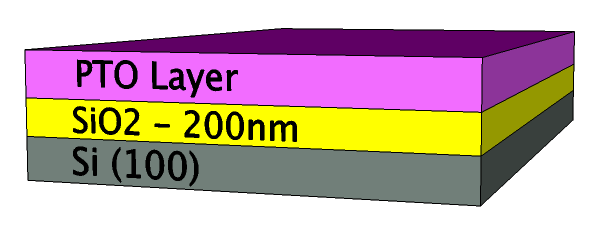
\includegraphics[width=0.75\textwidth]{./figures/DataAnalysis/ellipsometry-model-Si}
   \caption[Graphical Schematic of VASE Model]{A simple graphical example of the model used for %
   					analysis of the film stack in the Si(100) samples. The parameters %
					are $t$ and the spectroscopic values of $\tilde{n}$ for the PTO layer.}
   \label{fig:Si(100)-model}
\end{figure}

%%%%%%%%%%%%%%%%

\subsection{Analysis Procedure}
\label{chap:Methods-Ellip-Analysis}

Once the data was collected, a specific series of steps was followed in order to obtain the highest degree of accuracy from the model. All steps were performed on the PTO layer. The modeling procedure went as follows:

\begin{enumerate}
\item
High-$\lambda$ Cauchy Model
\item
Direct Calculation of $n$ and $\kappa$
\item
Conversion to Oscillator Model
\item
Refinement of Oscillator Layer Parameters
\end{enumerate}

This first step takes advantage of the transparency of the film at high wavelengths (low energies) where the photon energy is below the optical bandgap of the material. In this region, the Cauchy model can be used. The Cauchy model is empirical rather than physically descriptive, and best used for amorphous materials such as polymeric films, however the assumptions required for reasonable accuracy are met when absorption in the film layer is minimized (therefore $\kappa(\lambda)\approx0$). The equations used in the Cauchy model are shown in equation~\vref{eq:cauchy}. Generally, analysis during this step was performed in the spectral region where $\lambda = 600-1000$ nm ($E_{ph} = 2.06-1.24$ eV). 

\begin{subequations}
\label{eq:cauchy}
\begin{align}
	n\left(\lambda\right) &= A_{n} + \frac{B_{n}}{\lambda^{2}}+\frac{C_{n}}{\lambda^{4}}+\cdots\\
        	\kappa\left(\lambda\right) &= A_{\kappa}e^{B_{\kappa}\left(\frac{hc}{\lambda}\right)-C_{\kappa}}
\end{align}
\end{subequations}

Once reasonable estimates for $n$, $\kappa$, and the film layer thickness are obtained at the higher wavelengths, the second step of the analysis is to generate values of $\tilde{n}$ for the rest of the spectrum. The film thickness parameter is fixed at the value determined from the Cauchy model. The values of $n$ and $\kappa$ are allowed to be determined freely without the use of a model (i.e. directly determined by use of the Fresnel relations). This type of modeling is not physical, but assists in the generation of the oscillator-based model in the next step. The software package is then instructed to run a point-by-point fit of the data from highest- to lowest-$\lambda$, attempting to minimize the change in $n$ or $\kappa$ between adjacent data points. 

This model is then inputted into a oscillator model. For the analysis of these films, a Tauc-Lorentz oscillator model was utilized. The oscillator models used by WVASE32 are expressed in terms of the complex dielectric function $\tilde{\epsilon}$, which relates to $\tilde{n}$ via the relationship in equation~\vref{eq:dielectric}. The Tauc-Lorentz model changes the Lorentzian model by allowing for some absorption below the fundamental bandgap energy, which would be due to defect states and other intra-band transition mechanisms. The Tauc-Lorentz model uses the parameterization shown in equation~\vref{eq:TaucLorentz}\cite{WVASE-manual,Jellison96}. $\epsilon_{1}$ is provided here in a condensed version (eq.~\vref{eq:TaucLorentz-1}); the full expanded version, and its derivation via Kramers-Kronig integration (whose relations are shown in equation \vref{eq:KK-relation}) from $\epsilon_{2}$, has been presented by Jellison and Modine\cite{Jellison96}. 

\begin{subequations}
\label{eq:dielectric}
\begin{align}
	\tilde{\epsilon} &= \epsilon_{1}+i\epsilon_{2} = \tilde{n}^{2}\\
	\epsilon_{1} &= n^{2} - \kappa^{2}\\
	\epsilon_{2} &= 2n\kappa 
\end{align}
\end{subequations}

\begin{subequations}
\label{eq:TaucLorentz}
\begin{align}
	\label{eq:TaucLorentz-1}
	\epsilon_{1}=\frac{2}{\pi}P\int^{\infty}_{E_{g}}\frac{\xi\epsilon_{2}\left(\xi\right)}{\xi^{2}-E^{2}}\,%
				\mathrm{d}\xi & \hspace{2.5cm}
\end{align}
\begin{empheq}[left=\empheqlbrace]{align}
	\epsilon_{2} (E) = \frac{AE_{0}C\left(E-E_{g}\right)^{2}}{\left(E^{2}-E^{2}_{0}\right)^{2}+C^{2}E^{2}}%
		\cdot \frac{1}{E} && E> E_{g}\\
        	\epsilon_{2} (E) = 0 && E\leq E_{g}
\end{empheq}
\end{subequations}\\

\begin{subequations}
\label{eq:KK-relation}
\begin{align}
	\epsilon_{1}\left(\omega\right)-1&=\frac{2}{\pi}P\int^{\infty}_{0}\frac{\omega^{\prime}\epsilon_{2}\left(\omega^{\prime}\right)}{\omega^{\prime2}-\omega^{2}}d\omega^{\prime}\\
	\epsilon_{2}\left(\omega\right)&=-\frac{2\omega}{\pi}P\int^{\infty}_{0}\frac{\epsilon_{1}\left(\omega^{\prime}\right)-1}{\omega^{\prime2}-\omega^{2}}d\omega^{\prime}
\end{align}
\end{subequations}

\indent The WVASE32 software package allows one to use a graphical interface to provide initial guesses for the various fit parameters. At times this required multiple oscillators to best fit the predicted $\epsilon_{2}$ function. Once this has been set, all of the parameters affecting $\epsilon_{2}$ ($A, E_{0}, C, E_{G}$) are marked to be included in the fit. The software is then instructed to perform a best-fit of the oscillator to $\epsilon_{2}$. Once this operation completes, the software is set to fit to $\epsilon_{1}$ and only the value of the $\epsilon_{1}$ offset is allowed to be fit. Finally, the software is set to optimize vs both $\epsilon_{1}$ and $\epsilon_{2}$, and all parameters are included. This completes the initial setup of the oscillator model. 

Finally, the model is set to also allow the layer thickness to be fit and a general fit to the entire experimental dataset is performed. This provides the best guess to the physical values of the film. The thickness calculated by this procedure matches very closely to measurements performed by other methods (e.g. SEM imaging or AFM measurement of a lithographically created step). 

If similar deposition parameters are utilized, it is possible to save the parameterized model for later use. This allows the analysis to be streamlined when the material is expected to remain constant, for example if tests of deposition at different layer thicknesses are performed. In this case, the material would have optical behavior very similar to the initial sample, and the oscillator model would be sufficiently close to valid parameters to be used directly for fits. All that would need to be adjusted initially would be the estimated layer thickness. If the fit fails to produce useful data, such as unreasonable values for any of the parameters or very large confidence intervals, it is recommended to proceed with the entire standard analysis procedure. 

Further analysis can be performed to estimate the bandgap of the layer, via Tauc plot analysis. The method requires the calculation of the absorption coefficient ($\alpha$) from the value of $k$ for the layer (see equation~\vref{eq:alpha}). $\alpha$ is usually provided in terms of cm$^{-1}$, so if the wavelength is provided in nanometers a corresponding factor of $10^{7}$ must be incorporated as well. Subsequently, a Tauc plot is constructed using a combination of $\alpha$ and the photon energy. For direct bandgap materials the Tauc parameter is given by $\left(\alpha E_{ph}\right)^{2}$. If the bandgap is of the indirect type, the function is changed to $\sqrt{\alpha E_{ph}}$. The bandgap parameter matches well to literature values (when using standard samples of well defined materials, such as a thin layer of titania). It must be noted that the bandgap that is calculated is the overall bandgap of the layer, which may be a combination of multiple phases or materials. 

\begin{equation}
	\label{eq:alpha}%
	\alpha = \frac{4\pi k}{\lambda}
\end{equation}

Experimental data sets, the resulting fitted models, and Tauc analyses for selected samples are presented in appendix~\vref{sup:Ellipsometry}.

%%%%%%%%%%%%%%%%%%%%%%%%%%%%%%%%%%%%%%%%%%%%%%%%%%%%
%%%%%%%%%%%%%%%%%%%%%%%%%%%%%%%%%%%%%%%%%%%%%%%%%%%%
%%%%%%%%%%%%%%%%%%%%%%%%%%%%%%%%%%%%%%%%%%%%%%%%%%%%

\section{Composition Analysis}
\label{sec:Methods-Comp}

In order for the desired phase to be preferred, without any impurity phases precipitating, it is important to be able to control the stoichiometry of the produced film. Previous reports have shown that there is a close relationship between the composition of the film and the final resultant phase (see figure~\vref{fig:PTO-phase}).\cite{harjuoja_2006} 

\begin{figure}[tb]
   \centering
   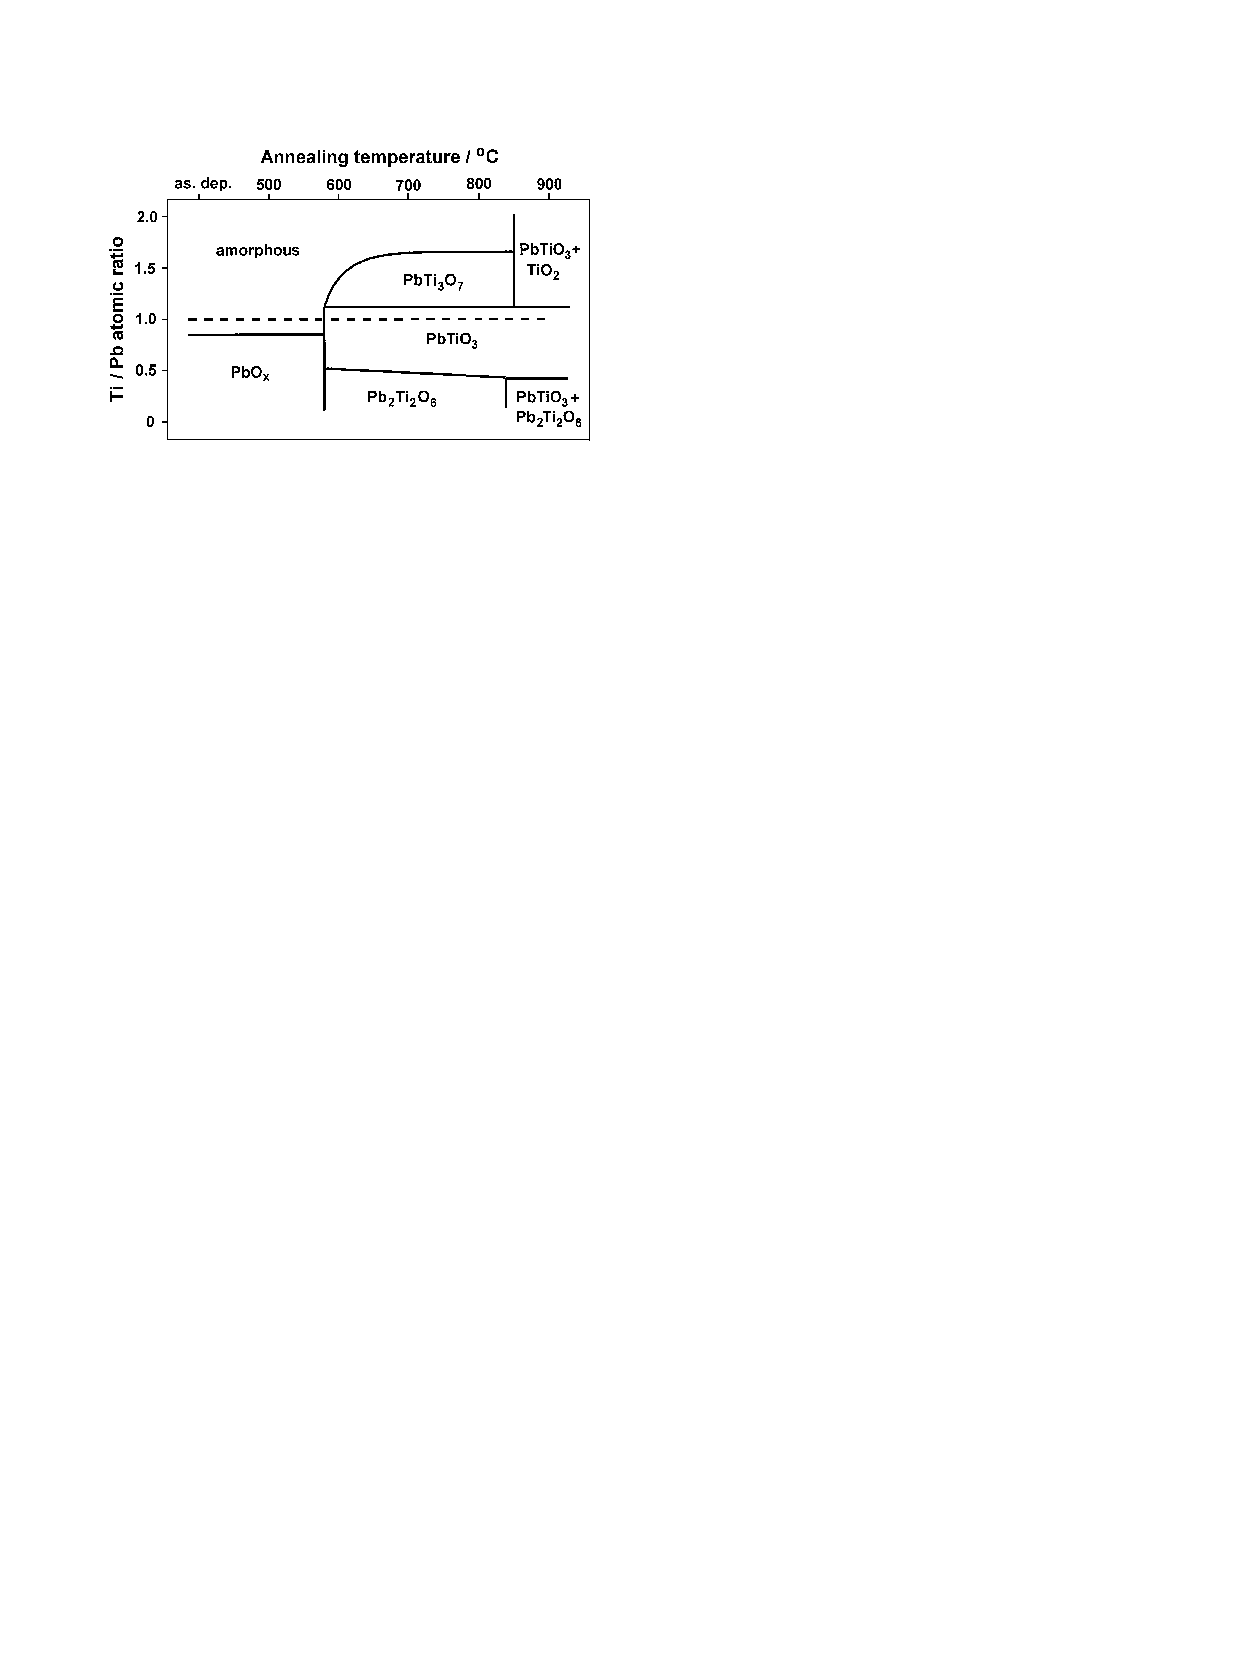
\includegraphics[width=0.75\textwidth]{./figures/dataanalysis/PTO-phase}
   \caption[Preferred Phase vs. Stoichiometric Ratio]{Graphic illustrating preferred phase of an annealed %
   		film at a range of stoichiometric ratios and annealing temperatures. A slight excess of \ce{Pb} %
		in the system is expected to help stabilize the perovskite \PTO{} phase.\cite{harjuoja_2006}}
   \label{fig:PTO-phase}
\end{figure}

\lipsum

%%%%%%%%%%%%%%%%

\subsection{X-Ray Fluorescence Spectroscopy}
\label{sec:Methods-XRF}

X-ray Fluorescence was the primary method used for determining the composition of the deposited films. Analysis was performed in a scanning electron microscope (FEI Strata DB235). The sample was imaged in order to identify the exact height of the sample within the chamber, via the microscope's focal length. After the sample had been properly positioned, the imaging beam was disengaged and the X-ray source activated. Then, in much the same manner as EDS, the emitted X-rays are collected and analyzed. A target X-ray count was around 20,000-50,000 for most samples. If the film on a particular sample was found to be very thin, more counts were often required to obtain well-defined peaks for the film elements. 

Initial calibration of the system is critically important to acquiring accurate measurements. Calibration is performed using a pair of standard samples of known composition, which include all elements that are to be quantified. For this study, a pellet of commercially prepared \PTO{} powder and a thin film of \ce{PbZr_{0.52}Ti_{0.48}O3} were used as standards. 

The only major issue with XRF --- and composition analysis in general --- that was encountered during the course of this work was the fact that it was not surface sensitive. In fact, many of the observed counts could be attributed to the substrate. In general this proved not to be problematic, but when the sample and film had elements in common this analysis was confounded and completely impossible to perform using XRF. This was the case with PTO films deposited on \ce{SrTiO3} substrates, as both the film and the substrate had titanium content. 

This issue could have been circumvented by using surface-sensitive techniques; examples of these methods include Auger electron spectroscopy (AES), X-ray photoelectron spectroscopy (XPS), and Rutherford backscattering spectroscopy (RBS). Unfortunately, none of these tools were available at the time and as such samples deposited on STO do not have associated composition information. 

%%%%%%%%%%%%%%%%%%%%%%%%%%%%%%%%%%%%%%%%%%%%%%%%%%%%
%%%%%%%%%%%%%%%%%%%%%%%%%%%%%%%%%%%%%%%%%%%%%%%%%%%%
%%%%%%%%%%%%%%%%%%%%%%%%%%%%%%%%%%%%%%%%%%%%%%%%%%%%

\section{X-Ray Diffraction}
\label{sec:Methods-XRD}

X-ray diffraction (XRD) was used in this study to investigate the phases that crystallized in the samples after annealing treatments were performed.  Sample alignment was an automated, preprogrammed process for film-type structures; the system performed alignments on all available axes to ensure optimum sample placement and orientation. Calibration of the system was managed by lab technicians. 

Data was collected in the standard $\theta-2\theta$ orientation, and was programmed to sweep ranges between 10--90$^{\circ}$. Varying time constants were used on different samples, as samples with thicker ALD films supplied a stronger signal. 

%%%%%%%%%%%%%%%%

%\subsection{Grazing Incidence XRD}
%
%For each sample, the value of $\omega$ was set to be 80\% of the film's critical angle which was determined prior to the scan. 






\chapter{Results}
\label{ch:Results}
\thispagestyle{empty}

%%%%%%%%%%%%%%%%%%%%%%%%%%%%%%%%%%%%%%%%%%%%%%%%%%%%%%%%%%
%%%%%%%%%%%%%%%%%%%%%%%%%%%%%%%%%%%%%%%%%%%%%%%%%%%%%%%%%%
%%%%%%%%%%%%%%%%%%%%%%%%%%%%%%%%%%%%%%%%%%%%%%%%%%%%%%%%%%

As discussed, the goal of this study was to determine methods for atomic layer deposition of ferroelectric oxides. In the process of realizing this goal there were a number of different areas of study. The first is the analysis of thermal and chemical behavior of the various potential precursors, during which TGA and DSC were primarily used (see~\vref{sec:Methods-Thermal}). Secondly,  the analysis of the film growth behavior under various conditions, this was primarily measured and analyzed using the ellipsometric techniques discussed earlier (see~\vref{sec:Methods-Ellip}). Third, the film deposition needed to be tuned to produce films with a stoichiometric composition, as this was expected to produce films which would crystallize into the desired perovskite phase, see section~\vref{sec:Methods-Comp} for the methods used for this characterization. Fourth, the phase of the crystallized film was analyzed in detail to determine behavior of the films post-annealing. XRD was used extensively for this task (see~\vref{sec:Methods-XRD}).


%%%%%%%%%%%%%%%%%%%%%%%%%%%%%%%%%%%%%%%%%%%%%%%%%%%%%%%%%%
%%%%%%%%%%%%%%%%%%%%%%%%%%%%%%%%%%%%%%%%%%%%%%%%%%%%%%%%%%
%%%%%%%%%%%%%%%%%%%%%%%%%%%%%%%%%%%%%%%%%%%%%%%%%%%%%%%%%%

\section{Thermal Analysis}
\label{chap:Results-Thermal}

While a viable titanium precursor was well identified in literature as well as experimentally, as was the oxidizers that were used, there was no such universally accepted chemical used in ALD to provide a source of lead. The primary issue was either a lack of chemical stability or a undesirably low volatility in the compounds that currently were being used. TGA and DSC was performed on a number of potential candidates (see~\vref{sec:SampFab-Precursors} for more details) in order to gauge the performance of these materials. 

%%%%%%%%%%%%%%%%

\subsection{Thermogravimetric Analysis}

Thermogravimetric analysis allows for the estimation and comparison of volatility between multiple samples. It was used in this study primarily to compare properties of the two candidate precursors, \HFAc{} and \TMHD{}. Of primary consideration was the volatility of the compound --- evaluated qualitatively by analyzing the mass loss at various temperatures --- and whether or not there are indications of imperfect evaporation. The data collected for these materials can be found below. 

By analyzing the TGA curve for \HFAc{}, found in figure~\vref{fig:TGA-HFAc-Weight}, there are a number of features that are immediately noticeable. First of these is the presence of multiple stages of evaporation in the curve. These occur at approximately 170 and 190\degC{}. A TGA curve for a material that is purely evaporative, e.g. pure water, will have a smooth curve. Additional steps indicate that other processes are activating, and causing changes to the compound affecting the mass loss. 

More detail can be seen by performing a derivation on the TGA curve, giving the mass loss rate. This plot can be found in figure~\vref{fig:TGA-HFAc-DWeight}. This plot shows a shoulder on the primary evaporative peak, and then another peak starting at around 170\degC{} and peaking at 190\degC{}. The shoulder indicates that even during the evaporation of the bulk of the material, before residues and other imperfections cause rate changes, a secondary mechanism is activating and impacting the mass loss rate. 

\begin{figure}[tbp]
   \centering
   \subfloat[Mass vs. Temperature][Mass vs. Temperature]{%
   	\label{fig:TGA-HFAc-Weight}%
	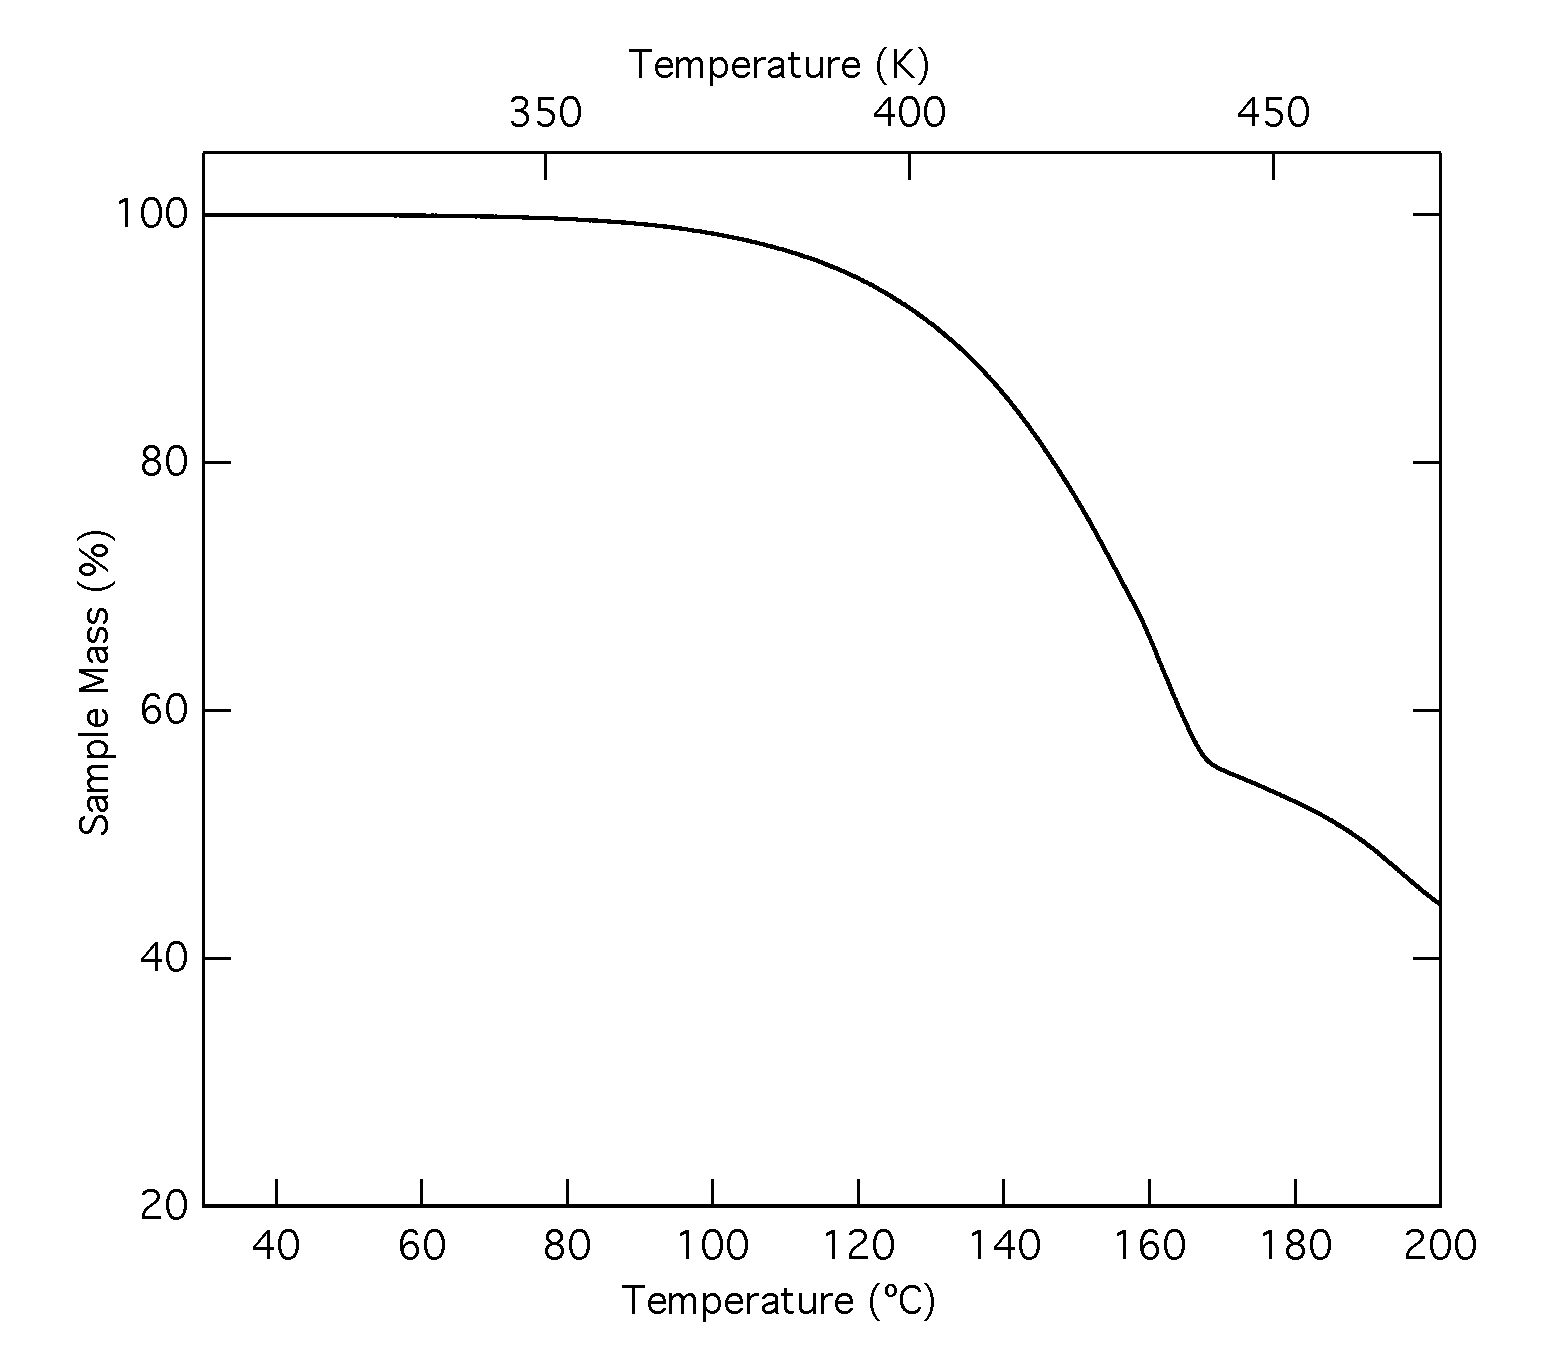
\includegraphics[width=0.45\textwidth]{./Figures/Data/Thermal-Analysis/TGA/HFAc-Weight}%
	}
	\hspace{1cm}
  \subfloat[Derivative of Mass vs. Temperature][Derivative of Mass vs. Temperature]{%
   	\label{fig:TGA-HFAc-DWeight}%
	\includegraphics[width=0.45\textwidth]{./Figures/Data/Thermal-Analysis/TGA/HFAc-DWeight}%
	} 	
   \caption[TGA Results for Pb(HFAc)$_{2}$ Precursor]%
   		{Plots of the results from TGA experiments on Pb(HFAc)$_{2}$. The plot shown in (a) gives the raw %
		data showing the current mass as a function of temperature. (b) gives the same data, transformed %
		to show the derivative of mass. Thus (b) shows the rate of mass loss at a given temperature. Initial %
		sample mass: 6.092 mg}
   \label{fig:TGA-HFAc}
\end{figure}

Comparing this data with that of \TMHD{}, it is immediately obvious that the evaporation mechanism for the latter is much smoother. There is no major visible step, apart from some slight changes nearing the upper end of the testing temperature range (185--200\degC{}). With a closer look at figure~\ref{fig:TGA-TMHD-DWeight}, it is easier to see that there is smooth vaporization up to approximately 180\degC{}, at which point the evaporation is slowed dramatically due to residue buildup. 

\begin{figure}[tbp]
   \centering
   \subfloat[Mass vs. Temperature][Mass vs. Temperature]{%
   	\label{fig:TGA-TMHD-Weight}%
	\includegraphics[width=0.45\textwidth]{./Figures/Data/Thermal-Analysis/TGA/TMHD-Weight}%
	}
	\hspace{1cm}
  \subfloat[Derivative of Mass vs. Temperature][Derivative of Mass vs. Temperature]{%
   	\label{fig:TGA-TMHD-DWeight}%
	\includegraphics[width=0.45\textwidth]{./Figures/Data/Thermal-Analysis/TGA/TMHD-DWeight}%
	} 	
   \caption[TGA Results for Pb(HFAc)$_{2}$ Precursor]%
   		{Plots of the results from TGA experiments on Pb(TMHD)$_{2}$. As in figure~\vref{fig:TGA-HFAc}, (a) %
		presents the actual mass as a function of temperature, while (b) gives the derivative of that function. %
		Initial sample mass: 3.719 mg}
   \label{fig:TGA-TMHD}
\end{figure}

Neither of these precursors evaporated cleanly, leaving residues of more than 20\% of their initial sample mass during the temperature scanning tests discussed above. When these were tested at moderate temperatures, such as those to be used for evaporation in the ALD system, both left even larger fractions of their initial masses behind. Testing at a constant temperature (160\degC{}) over a longer period of time gives the plots shown in figure~\vref{fig:TGA-Hold}. From this test, it was found that \HFAc{} left a much larger residue than \TMHD{}, 63\% and 34\% respectively. 

\begin{figure}[tbp]
   \centering
   \subfloat[\HFAc][\HFAc]{%
   	\label{fig:TGA-HFAc-Hold}%
	\includegraphics[width=0.45\textwidth]{./Figures/Data/Thermal-Analysis/TGA/HFAc-Hold}%
	}
	\hspace{1cm}
  \subfloat[\TMHD][\TMHD]{%
   	\label{fig:TGA-TMHD-Hold}%
	\includegraphics[width=0.45\textwidth]{./Figures/Data/Thermal-Analysis/TGA/TMHD-Hold}%
	} 	
   \caption[Constant Temperature TGA Experiments]%
   		{Plots of the results from ramp-and-hold TGA experiments designed to investigate residual material %
		after complete evaporation at a given temperature. From the TGA experiments seen above (figs.~%
		\vref{fig:TGA-HFAc} and \vref{fig:TGA-TMHD}), a common temperature of 160\degC{} was chosen %
		for this experiment. Sample masses were 3.921 mg and 4.381 mg for \HFAc{} and \TMHD{} respectively.}
   \label{fig:TGA-Hold}
\end{figure}

Based on the results of these tests, the lower residual mass and the cleaner evaporative process, \TMHD{} was predicted to have better performance as an ALD precursor. 

%%%%%%%%%%%%%%%%

\subsection{Differential Scanning Calorimetry}

As discussed in previous chapters, DSC is a powerful tool for analyzing the behavior of precursors. The data collected allows for the understanding of various energies in the material. 

When considering the energetic behavior of \HFAc{} (see fig.~\vref{fig:DSC-HFAc}), there are a few minor features that can be noticed. Primarily at 25 and 150\degC{} small peaks are visible that indicate changes in the material other than the solid to liquid phase change, which is the much larger peak seen around 155-160\degC{}. However, these peaks appear to be negligible, as the total energy release by the sample is a mere 5.32 mJ (1.13 J/g), which is too low for any major chemical changes to be occurring. 

\begin{figure}[htb]
	\centering
	\includegraphics[width=0.66\textwidth]{./Figures/Data/Thermal-Analysis/DSC/HFAc}
	\caption[DSC Results of \HFAc{}]%
		{Plot of the DSC scan of \HFAc{}. In this plot exothermic behavior, where the sample releases heat, is %
		considered positive. Thus, the first sweep of the scan (from 0\degC{} to 200\degC{}) is negative. %
		Sample mass: 4.7 mg.}
	\label{fig:DSC-HFAc}
\end{figure}

Similarly, when \TMHD{} is heated to moderate temperatures (up to 200\degC{}, see fig~\vref{fig:DSC-TMHD-200}), such as those used in the evaporation and transport stages of the ALD system, there are no irregularities in the data. There is also no net energy gain or loss during the test indicating that heating up to 200\degC{}, along with the associated melting and freezing of the compound, is not detrimental to its structure. 

If the test is again performed, but with a higher upper temperature bound, the data is drastically different (see fig.~\vref{fig:DSC-TMHD-300}). As the sample is heated up to 300\degC{}, there are a number of significant energy releases that occur. These processes initiate at 234\degC{}, and are due to the precursor undergoing pyrolysis reactions. As such, this sets the safe upper temperature range for the ``ALD window'' of \TMHD{} at 230\degC{}. ALD reactions require that the precursor arrive to the surface intact and only react with surface species present. 

\begin{figure}[tbp]
	\centering
	\subfloat[][Low Temperature Test (30--200--30\degC{})]{\label{fig:DSC-TMHD-200}%
		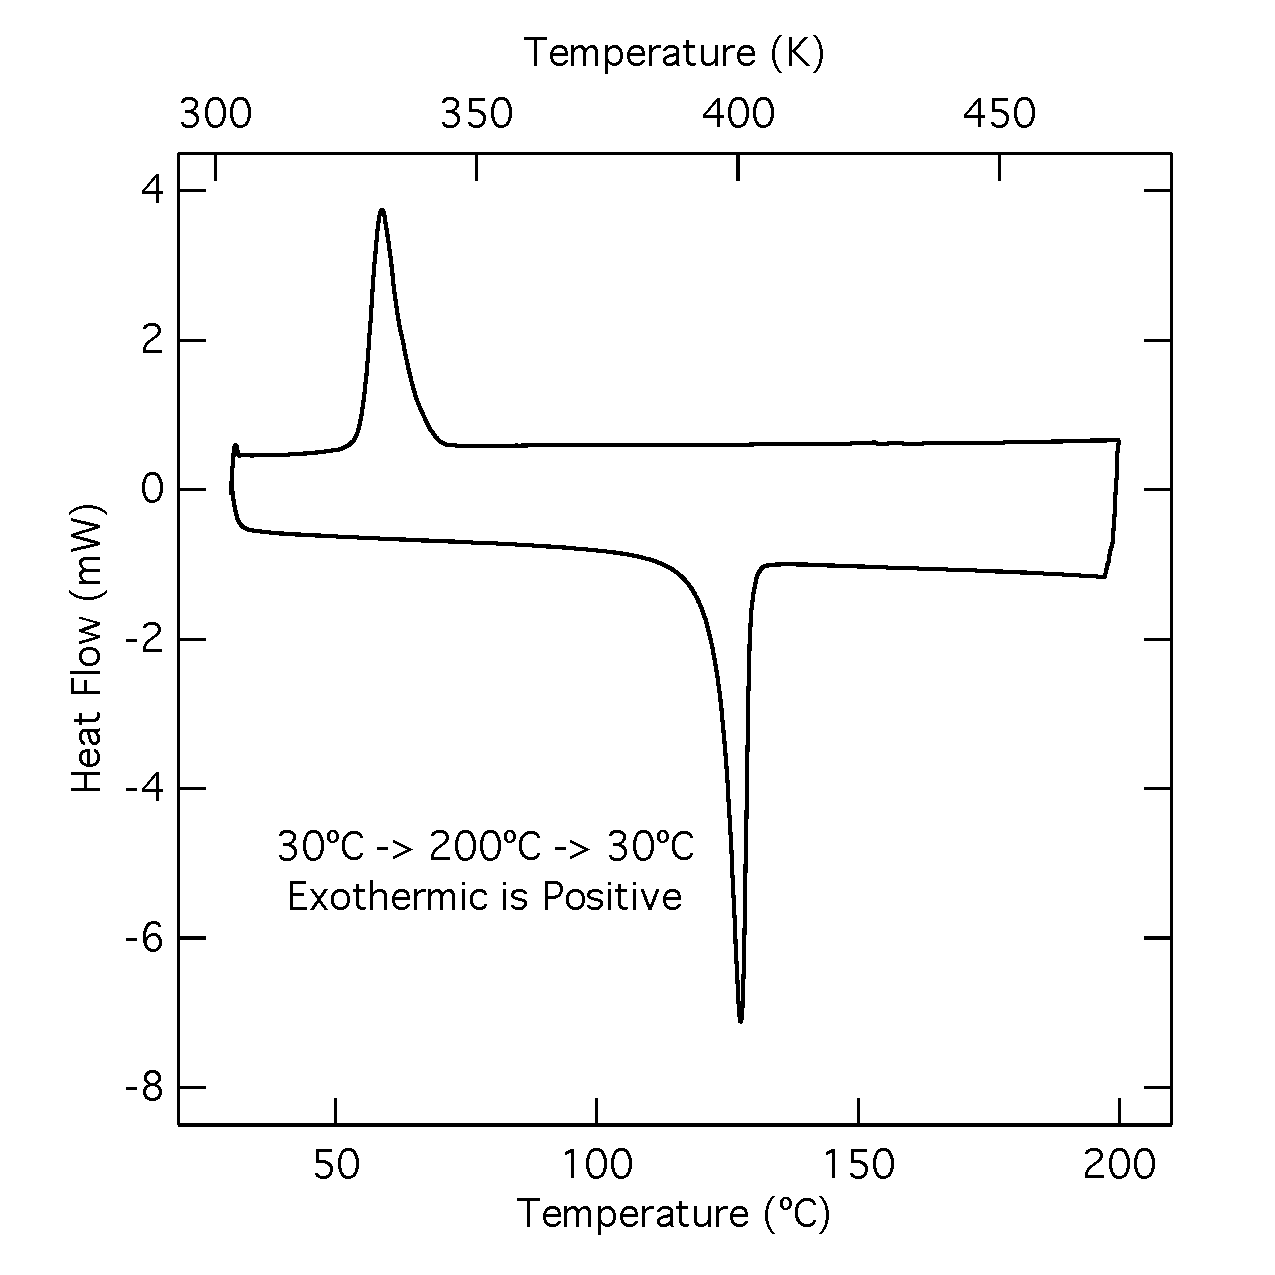
\includegraphics[width=0.66\textwidth]{./Figures/Data/Thermal-Analysis/DSC/TMHD-200}%
		}\\
	%\hspace{0.5cm}
	\subfloat[][High Temperature Test (30--300-30\degC{})]{\label{fig:DSC-TMHD-300}%
		\includegraphics[width=0.66\textwidth]{./Figures/Data/Thermal-Analysis/DSC/TMHD}%
		}
	\caption[DSC Results of \TMHD{}]%
		{Results from the DSC scans of \TMHD{}. (a) Temperatures up to 200\degC{} show no change in the %
		material other than that of melting and freezing. (b) As temperatures increase, features start to appear %
		indicating chemical reconfiguration of the molecule.}
	\label{fig:DSC-TMHD}
\end{figure}
\clearpage
%%%%%%%%%%%%%%%%%%%%%%%%%%%%%%%%%%%%%%%%%%%%%%%%%%%%%%%%%%
%%%%%%%%%%%%%%%%%%%%%%%%%%%%%%%%%%%%%%%%%%%%%%%%%%%%%%%%%%
%%%%%%%%%%%%%%%%%%%%%%%%%%%%%%%%%%%%%%%%%%%%%%%%%%%%%%%%%%

\section{List of Samples}
\label{chap:Results-Samples}

Based on the results from the thermal analysis, a number of samples were deposited with various deposition parameters. Information on the deposition parameters for each of the samples used in this study can be found in the following table~\vref{tbl:LoSamples}. A small number of samples were attempted at 200\degC{}, but it was quickly determined that 225\degC{} provided better growth behavior without risking thermal cracking of the precursor. 

{\small
\begin{longtable}{cccccccc}
	\caption[List of Samples]{A list of samples produced during the course of this project.%
	\label{tbl:LoSamples}}\\
	\toprule
	&&&&&\multicolumn{3}{c}{Annealing}\\ \cmidrule{6-8}
	Temp.		&Run \#	&Pb:Ti	 	&Cycles 	&Subs. 	&Type	&Temp. 		&Time\\ 
	(\degC{})		&		&Ratio		&		&Type	&		&(\degC{})	&(min)\\ \midrule%
	\endfirsthead
	\caption[]{A list of samples used during the course of this project.}\\
	\toprule
	&&&&&\multicolumn{3}{c}{Annealing}\\ \cmidrule{6-8}
	Temp.		&Run \#	&Pb:Ti	 	&Cycles 	&Subs. 	&Type	&Temp. 		&Time \\ 
	(\degC{})		&		&Ratio		&		&Type	&		&(\degC{})	&(min) \\ \midrule%
	\endhead
	200	&3		&1:1		&250	&Si		&None	&N/A		&N/A		\\
		&2		&1:2		&250	&Si		&None	&N/A		&N/A		\\
		&30		&3:1		&160	&Si		&None	&N/A		&N/A		\\
		&		&		&		&Pt-Si	&None	&N/A		&N/A		\\ \midrule
	225	&0		&1:1		&625	&Si		&Oven	&650	&120	\\
		&		&		&		&		&Oven	&900	&120	\\
		&		&		&		&		&RTA	&900	&10		\\
		&1		&1:1		&475	&Si		&None	&N/A		&N/A		\\
		&6		&1:2		&250	&Si		&None 	&N/A		&N/A		\\
		&13		&3:1		&250	&Si		&None 	&N/A		&N/A		\\
		&16		&3:1		&150	&Si		&RTA	&650	&1		\\
		&19		&3:1		&100	&Si		&None 	&N/A		&N/A		\\
		&		&		&		&Pt-Si	&None 	&N/A		&N/A		\\
		&20		&3:1		&200	&Si		&None 	&N/A		&N/A		\\
		&		&		&		&Pt-Si	&Oven	&650	&90		\\
		&		&		&		&STO	&Oven	&650	&90		\\
		&21		&3:1		&150	&Si		&None 	&N/A		&N/A		\\
		&		&		&		&Pt-Si	&Oven	&650	&90		\\
		&		&		&		&STO	&Oven	&650	&90		\\
		&22		&3:1		&150	&Si		&None 	&N/A		&N/A		\\
		&		&		&		&Pt-Si	&Oven	&650	&90		\\
		&23		&3:1		&200	&Si		&None 	&N/A		&N/A		\\
		&		&		&		&Pt-Si	&Oven	&650	&90		\\
		&28		&3:1		&120	&STO	&Oven	&650	&90		\\
	\bottomrule
\end{longtable}}

%%%%%%%%%%%%%%%%%%%%%%%%%%%%%%%%%%%%%%%%%%%%%%%%%%%%%%%%%%
%%%%%%%%%%%%%%%%%%%%%%%%%%%%%%%%%%%%%%%%%%%%%%%%%%%%%%%%%%
%%%%%%%%%%%%%%%%%%%%%%%%%%%%%%%%%%%%%%%%%%%%%%%%%%%%%%%%%%

\section{Ellipsometry}
\label{chap:Results-Ellipsometry}

Ellipsometry was a valuable tool during the course of this study. As discussed previously, it is capable of quickly, accurately, and non-destructively determine various properties of thin film layer stacks. Of primary importance is the ability of the tool to provide a rapid method of determining the thickness of a deposited layer. In ALD the growth rate is one of the primary markers of a well-tuned deposition process. An uncontrollably high growth rate is nearly as detrimental as having minimal growth. Varying deposition parameters and noting their effects on the growth rate of the process provided valuable insight into how best to tune the process. 

Given in table~\ref{tbl:LoThicknesses} is information on various samples and their as-deposited layer thicknesses, along with some relevant deposition parameters. One can also see from the plot of the sample thicknesses with respect to the number of deposition cycles (fig.~\vref{fig:Ellip-rates}) the consistency of a growth rate given a certain set of parameters. There is a small number of initial cycles required to initiate growth, referred to as ``incubation'' cycles, and then the film thickness follows a close linear dependence to the number of deposition cycles. This is indicative of a deposition that is operating within the ALD window and behaving well. From figure~\ref{fig:Ellip-rates} it was found that films deposited on silicon required approximately 10 cycles to initiate layer growth and subsequently grew at a rate of 3.78 \AA/cycle. For platinum coated silicon the incubation time was longer, an average of 36 cycles, but the films grew at a faster rate of 4.12 \AA/cycle. On STO crystals a 21 cycle incubation period was followed by a growth phase with a rate of 4.08 \AA/cycle. This varies greatly from values reported in table~\ref{tbl:LoThicknesses} as the growth rates reported here do not take into account the incubation time. The relatively constant number of initiation cycles has a seemingly greater effect on samples with low cycle counts; the incubation cycles take up a greater percentage of the total run and lower the growth rate accordingly. 

\begin{table}[tbp]
	\centering
	\small
	\caption[Sample Thicknesses and Growth Rates]%
		{Table of the film thicknesses and associated growth rates as measured by ellipsometry. Growth rates do %
		not take into account any incubation times for the films.}
	\label{tbl:LoThicknesses}
	\begin{tabular}{llllrr}
		\toprule
		Pb:Ti		&Sample	&Cycles		&Substrate	&Thickness	&Growth Rate	\\
		Ratio	&\#		&			&Type		&(nm)		&(\AA/cycle)	\\ \midrule
		1:1		&0		&625		&Si			&85.9		&1.37		\\
				&1		&475		&Si			&63.4		&1.33		\\
		3:1		&13		&250		&Si			&*32.9		&*1.31		\\
				&16		&150		&Si			&51.2		&3.41		\\
				&19		&100		&Si			&34.3		&3.43		\\
				&		&			&Pt-Si		&27.5		&2.75		\\
				&20		&200		&Si			&71.8		&3.59		\\
				&		&			&Pt-Si		&64.4		&3.22		\\
				&		&			&STO		&73.6		&3.68		\\
				&21		&150		&Si			&53.2		&3.54		\\
				&		&			&Pt-Si		&45.8		&3.05		\\
				&		&			&STO		&52.9		&3.53		\\
				&22		&150		&Si			&53.3		&3.55		\\
				&		&			&Pt-Si		&46.5		&3.10		\\
				&23		&200		&Si			&72.0		&3.60		\\
				&		&			&Pt-Si		&64.6		&3.23		\\
				&28		&120		&STO		&41.0		&3.42		\\	
		\bottomrule
	\end{tabular}
\end{table}

\begin{figure}[tbp]
	\centering
	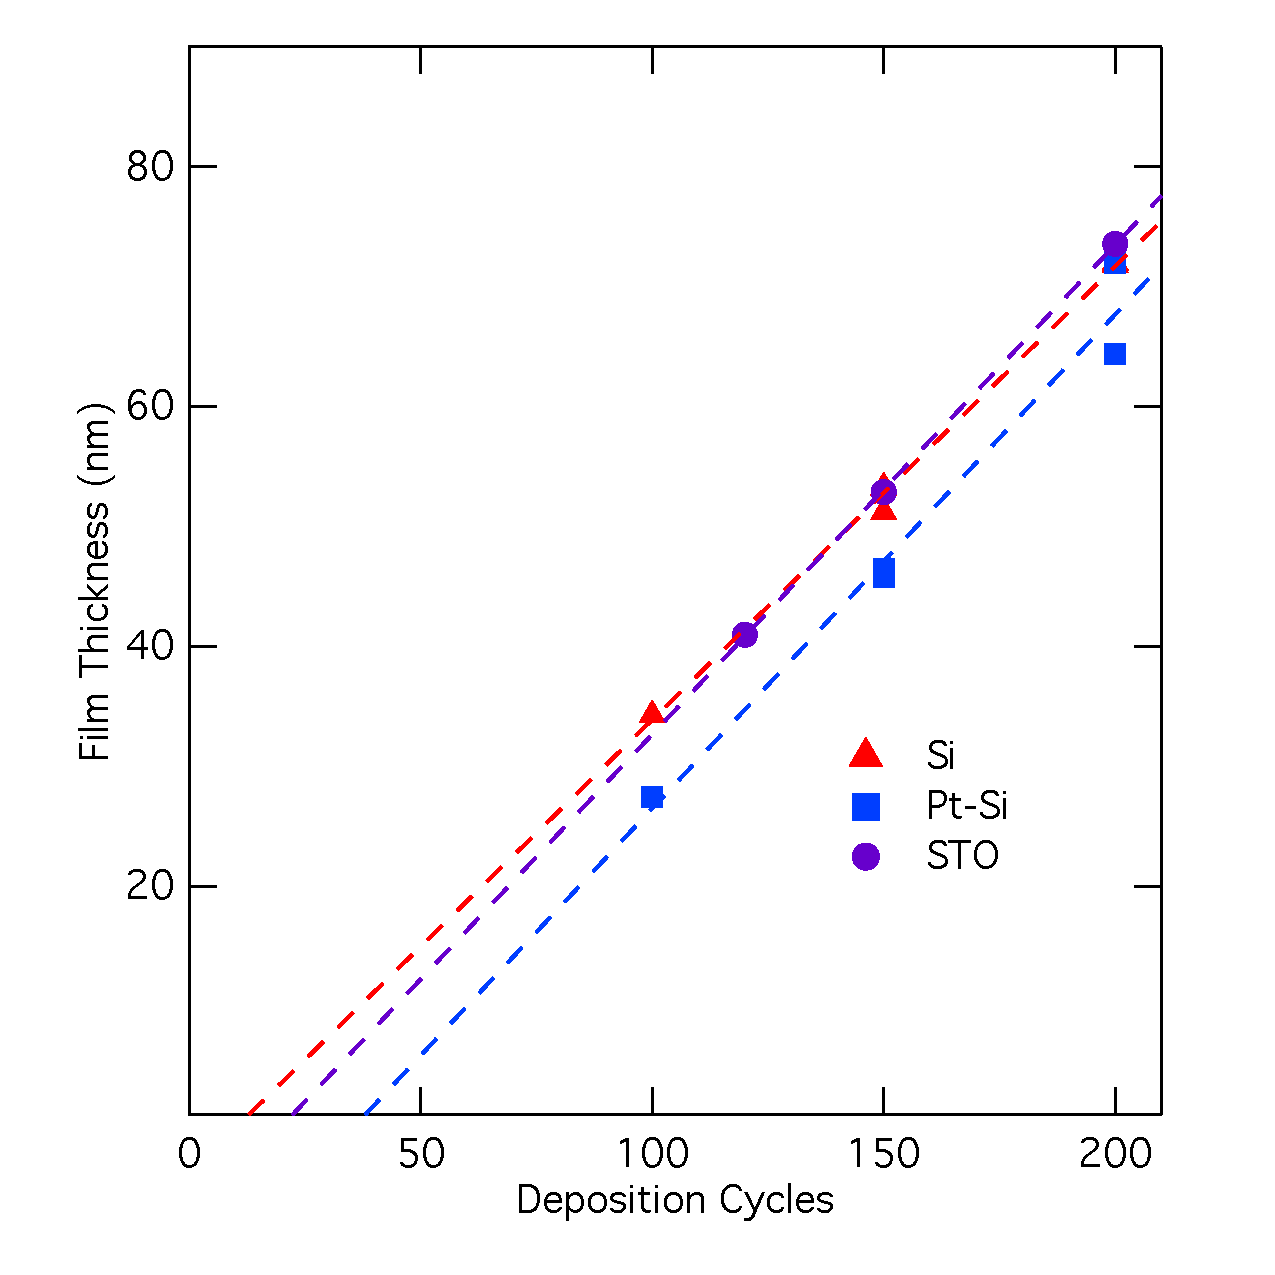
\includegraphics[width=0.6\textwidth]{./Figures/Data/Ellipsometry/Ellip-Rates}
	\caption[Film Thicknesses vs. Deposition Cycles]%
		{A plot of film thicknesses determined by ellipsometry. Growth rates and average incubation times are %
		extrapolated from this data. All films were deposited with a 3:1 Pb:Ti ratio and at 225\degC{}}
	\label{fig:Ellip-rates}
\end{figure}
	
An additional piece of information that can be extracted from ellipsometric analysis is an estimation of the band gap energy of the deposited layer. Because the final model used in the analysis method (see section~\vref{chap:Methods-Ellip-Analysis}) is physically descriptive of the optical properties of the material, it is possible to extract such information from the model. By transforming the plot of the extinction coefficient, $k$, into that of the absorption coefficient, $\alpha$, it becomes possible to use the method developed by Tauc, \emph{et.al.} \reword{[citation needed]} to determine the band gap energy of the material. However, such analysis does not take into account presence of multiple phases in the layer and takes a weighted average of the bandgaps. It also requires that the sample be properly crystallized, and thus must have undergone an annealing treatment before the analysis method becomes valid. However, since the samples produced here had low phase purity, which will be discussed in subsequent sections, this analysis was of little use as a film benchmark. Some results from these analyses can be found in section~\vref{sup:Ellipsometry}.

%%%%%%%%%%%%%%%%%%%%%%%%%%%%%%%%%%%%%%%%%%%%%%%%%%%%%%%%%%
%%%%%%%%%%%%%%%%%%%%%%%%%%%%%%%%%%%%%%%%%%%%%%%%%%%%%%%%%%
%%%%%%%%%%%%%%%%%%%%%%%%%%%%%%%%%%%%%%%%%%%%%%%%%%%%%%%%%%

\section{Composition}
\label{chap:Results-Composition}

Controlling the composition of the film was another primary task during the course of this project. Controlling the stoichiometry of the deposited films was of critical importance in obtaining films that presented the perovskite phase. If the balance of the two cations (\PbIon{} and \TiIon{}) was allowed to stray away from unity, other phases would be preferred or a mixture of phases would precipitate during a crystallizing heat treatment.  

As discussed previously, X-ray fluorescence was the method used for performing the composition analysis of the film structures. Through testing it was found that a deposition ratio of 3:1 in favor of the lead half-reaction provided the best film composition; there were a pair of samples deposited at an even 1:1 ratio that also provided near unity compositions (sample \#0 and \#1). A list of samples and their compositions, measured via XRF, can be found below (see table~\vref{tbl:XRF-compositions}). 

As mentioned in section~\ref{sec:Methods-XRF}, samples deposited on STO were unable to have their compositions accurately measured using this technique. This was due to the confounding influence of the titanium content in the STO substrate, and there were no surface sensitive characterization methods available. 


\begin{table}[tbp]
	\centering
	\caption[XRF Calculated Compositions]{Calculated compositions of selected samples, determined via XRF. \\Composition percentages are all $\pm$1\%.}\label{tbl:XRF-compositions}
	\begin{tabular}{l l r r r}
	\toprule
	&&\multicolumn{3}{c}{Composition (\%)}\\
	\cmidrule{3-5}
	Run \#&Substrate&Lead&Titanium&Ti:Pb Ratio\\
	\midrule
% 	Run	Sub-Type		Pb%		Ti%		Ti:Pb ratio
	0	&\ce{SiO2}	&56.0	&44.0	&0.786\\
	1	&\ce{SiO2}	&55.0	&45.0	&0.809\\
	13	&\ce{SiO2}	&54.0	&46.0	&0.853\\
	16	&\ce{SiO2}	&49.4	&50.6	&1.022\\
	19	&\ce{SiO2}	&65.9	&34.1	&0.518\\
		&Pt-Si		&42.9	&57.1	&1.333\\
	20	&\ce{SiO2}	&56.6	&43.4	&0.769\\
		&Pt-Si		&51.5	&48.5	&0.944\\
	21	&\ce{SiO2}	&69.6	&30.4	&0.437\\
		&Pt-Si		&56.1	&43.9	&0.783\\
	22	&\ce{SiO2}	&67.7	&32.3	&0.478\\
		&Pt-Si		&56.1	&43.9	&0.784\\
	23	&\ce{SiO2}	&66.9	&33.1	&0.495\\
		&Pt-Si		&49.1	&50.9	&1.038\\
	24	&\ce{SiO2}	&69.0	&31.0	&0.450\\
		&Pt-Si		&62.2	&37.8	&0.609\\
	\bottomrule
	\end{tabular}
\end{table}
\clearpage
%%%%%%%%%%%%%%%%%%%%%%%%%%%%%%%%%%%%%%%%%%%%%%%%%%%%%%%%%%
%%%%%%%%%%%%%%%%%%%%%%%%%%%%%%%%%%%%%%%%%%%%%%%%%%%%%%%%%%
%%%%%%%%%%%%%%%%%%%%%%%%%%%%%%%%%%%%%%%%%%%%%%%%%%%%%%%%%%


\section{X-Ray Diffraction}
\label{chap:Results-XRD}


XRD was performed on a number of samples that had indicated composition ratios near unity. After an annealing treatment, generally performed in a regular ambient environment furnace but occasionally through use of the RTA. However, samples processed using the RTA tended to obtain a unique and very rough surface texture, as opposed to the smooth mirror appearance of samples processed in the standard furnace. This observation lead to the adoption of the standard furnace as the main method of heat treatment. 


Insets of collected data sets, enlarged to allow for better visual identification of peaks and their locations, are presented here. Full data sets are provided in section~\vref{sup:XRD}. 



\begin{figure}[htbp]
	\subfloat[PTO (100) and PbO$_{2}$][PTO (100) and PbO$_{2}$]{%
   		\label{fig:XRD-20-Pt-20-27}%
		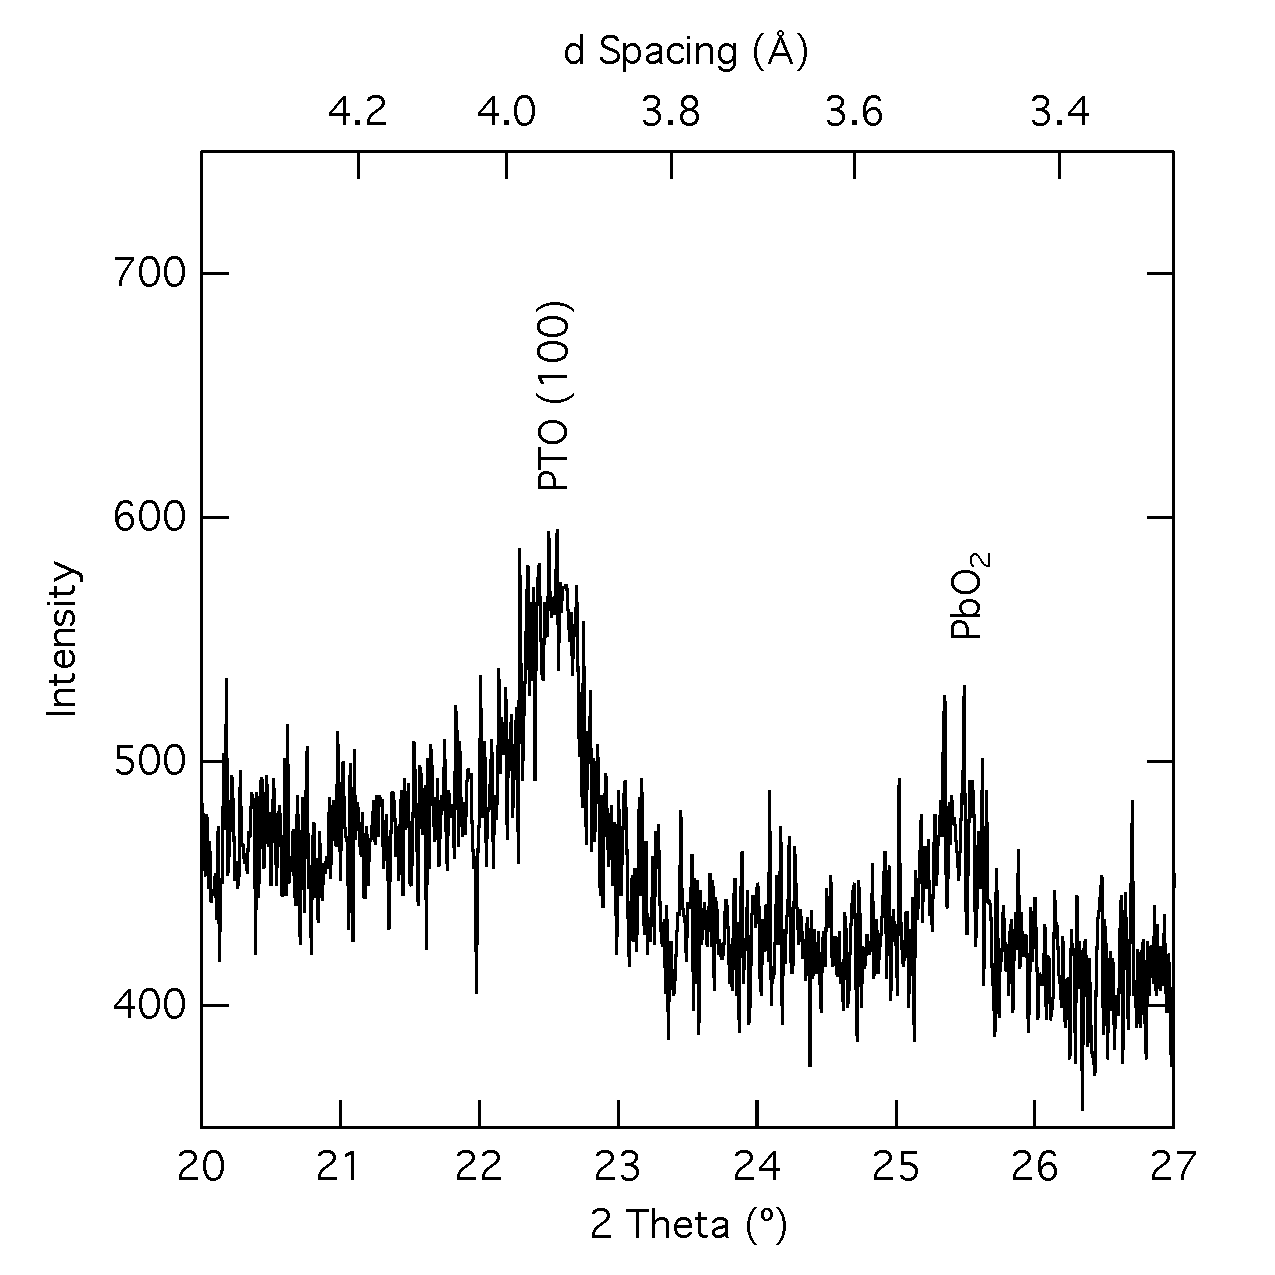
\includegraphics[width=0.47\textwidth]{./Figures/Data/XRD/Run-20-Pt/20-27.pdf}%
	} \hspace{0.5cm}
	\subfloat[PbO (220) and PTO (200)][PbO (220) and PTO (200)]{%
   		\label{fig:XRD-20-Pt-43-48}%
		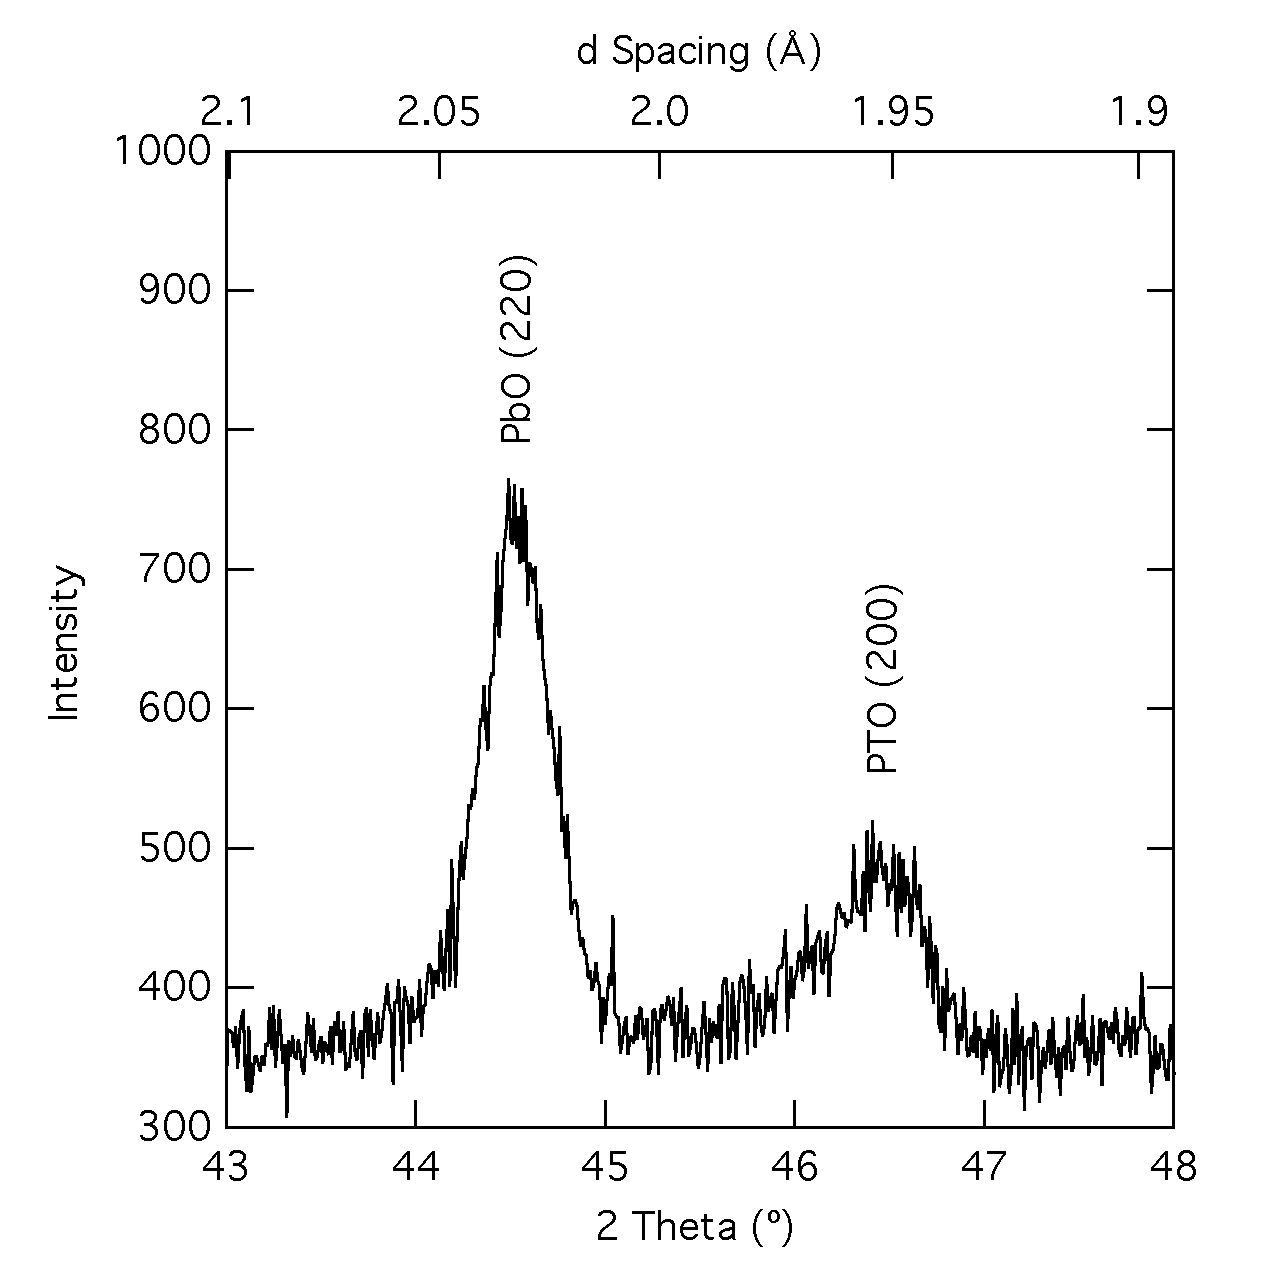
\includegraphics[width=0.47\textwidth]{./Figures/Data/XRD/Run-20-Pt/43-48.pdf}%
	}
\end{figure}




















\chapter{Conclusions}
\label{ch:Conc}
\thispagestyle{empty}

%%%%%%%%%%%%%%%%%%%%%%%%%%%%%%%%%%%%%%%%%%%%%%%%%%%%%%%%%%
%%%%%%%%%%%%%%%%%%%%%%%%%%%%%%%%%%%%%%%%%%%%%%%%%%%%%%%%%%
%%%%%%%%%%%%%%%%%%%%%%%%%%%%%%%%%%%%%%%%%%%%%%%%%%%%%%%%%%

\section{Future Work}
\label{sec:Conc-Future}

Optimize consistency

Doped materials

Other material systems (BFO, BST, etc.)


\lipsum











%%% END OF CONTENT %%%

\cleardoublepage % Start new odd page


% ---- Bibliography ----
\addcontentsline{toc}{chapter}{Bibliography} % Adds Bibliography chapter entry to ToC. 
\bibliographystyle{unsrt} % This will not sort the bibliography in anyway, but instead will sort by order of appearance in the document. Other styles available.

% Creates the bibliography from the file 'bib_thesis.bib'. Can reference multiple .bib files, just separate with commas
\bibliography{./bibliography/bib_thesis,./bibliography/bib_PTO} 


%\nocite{*}  	% This will add any remaining entries in the BibTeX file to the bibliography, without citing it in the document. 


\appendix

\pagestyle{fancy} 
\fancyfoot{}                                               
\renewcommand{\chaptermark}[1]{\markboth{\appendixname\ \thechapter.\ #1}{}} 
\renewcommand{\sectionmark}[1]{\markright{\thesection.\ #1}}         
\fancyhead[LE,RO]{\bfseries\thepage}    
                                        
\fancyhead[RE]{\bfseries\leftmark}    
\fancyhead[LO]{\bfseries\rightmark}     
\renewcommand{\headrulewidth}{0.3pt} 



\chapter{Supplemental Information}
\label{chap:appendix}
\thispagestyle{empty}

%%%%%%%%%%%%%%%%%%%%%%%%%%%%%%%%%%%%%%%%%%%%%%%%%%%%
%%%%%%%%%%%%%%%%%%%%%%%%%%%%%%%%%%%%%%%%%%%%%%%%%%%%
%%%%%%%%%%%%%%%%%%%%%%%%%%%%%%%%%%%%%%%%%%%%%%%%%%%%

\section{List of Chemicals}
\label{sup:LoChemicals}

\begin{table}[htbp]
	\centering
	\caption[List of Compounds]{List of chemical compounds used during the course of this study.}
	\label{tbl:LoCompounds}
	\begin{tabular}{llrrl}
		\toprule
		Chemical				&Chemical 			&CAS \#		&Molec.	&Source	\\ 
		Name				&Formula				&			&Weight	&		\\\midrule
		Lead(II) hexafluoro- 		&\ce{Pb(C5O2HF6)2}	&19648-88-5	&621.29	&Strem Chemicals, Inc.\\	
		acetylacetonate		\\
		Bis(2,2,6,6-tetramethyl	&\ce{Pb(C11H19O2)2}	&21319-43-7	&573.50	&Strem Chemicals, Inc.\\
		-3,5-heptanedionato)\\
		Lead(II)\\
		Titanium(IV)			&\ce{Ti[OCH(CH3)2]4}	&546-68-9	&284.25	&Strem Chemicals, Inc.\\
		i-propoxide\\\midrule
		Isopropyl Alcohol (IPA)	&\ce{(CH3)2CHOH}		&67-63-0		&60.10	&Alfa Aesar\\
		Acetone				&\ce{C3H6O}			&67-64-1		&58.08	&Alfa Aesar\\
		Buffered Hydrofluoric	&\ce{NH4F}-\ce{HF}		&7664-39-3	&N/A		&Alfa Aesar\\
		Acid (BHF)			&					&\& 12125-01-8\\
		Ozone				&\ce{O3}				&10028-15-6	&48.00	&\\
		\bottomrule
	\end{tabular}
\end{table}

\clearpage

%%%%%%%%%%%%%%%%%%%%%%%%%%%%%%%%%%%%%%%%%%%%%%%%%%%%
%%%%%%%%%%%%%%%%%%%%%%%%%%%%%%%%%%%%%%%%%%%%%%%%%%%%
%%%%%%%%%%%%%%%%%%%%%%%%%%%%%%%%%%%%%%%%%%%%%%%%%%%%

%\begin{landscape}
%\section{List of Samples}
%\label{sup:LoSamples}

%{
%\begin{longtable}{c c c c c c c c c}
%	\caption[List of Samples]{A list of samples used during the course of this project.%
%	\label{tbl:LoSamples}}\\
%	\toprule
%	&&&&&\multicolumn{3}{c}{Annealing}&\\ \cmidrule{6-8}
%	Temp.		&Run \#	&Pb:Ti	 	&Cycles 	&Subs. 	&Type	&Temp. 		&Time &XRD\\ 
%	(\degC{})		&		&Ratio		&		&Type	&		&(\degC{})	&(min) &\\ \midrule%
%	\endfirsthead
%	\caption[]{A list of samples used during the course of this project.}\\
%	\toprule
%	&&&&&\multicolumn{3}{c}{Annealing}&\\ \cmidrule{6-8}
%	Temp.		&Run \#	&Pb:Ti	 	&Cycles 	&Subs. 	&Type	&Temp. 		&Time &XRD\\ 
%	(\degC{})		&		&Ratio		&		&Type	&		&(\degC{})	&(min) &\\ \midrule%
%	\endhead
%	200	&3		&1:1		&250	&Si		&None	&N/A		&N/A		&No\\
%		&2		&1:2		&250	&Si		&None	&N/A		&N/A		&No\\
%		&30		&3:1		&160	&Si		&None	&N/A		&N/A		&No\\
%		&		&		&		&Pt-Si	&None	&N/A		&N/A		&No\\ \midrule
%	250	&0		&1:1		&625	&Si		&Oven	&650	&120	&Yes\\
%		&		&		&		&		&Oven	&900	&120	&Yes\\
%		&		&		&		&		&RTA	&900	&10		&No\\
%		&1		&1:1		&475	&Si		&None	&N/A		&N/A		&No\\
%		&6		&1:2		&250	&Si		&None 	&N/A		&N/A		&No\\
%		&13		&3:1		&250	&Si		&None 	&N/A		&N/A		&No\\
%		&16		&3:1		&150	&Si		&RTA	&650	&1		&No\\
%		&19		&3:1		&100	&Si		&None 	&N/A		&N/A		&No\\
%		&		&		&		&Pt-Si	&None 	&N/A		&N/A		&No\\
%		&20		&3:1		&200	&Si		&None 	&N/A		&N/A		&No\\
%		&		&		&		&Pt-Si	&Oven	&650	&90		&Yes\\
%		&21		&3:1		&150	&Si		&None 	&N/A		&N/A		&No\\
%		&		&		&		&Pt-Si	&Oven	&650	&90		&No\\ \\
%		&22		&3:1		&150	&Si		&None 	&N/A		&N/A		&No\\
%		&		&		&		&Pt-Si	&Oven	&650	&90		&Yes\\
%		&23		&3:1		&200	&Si		&None 	&N/A		&N/A		&No\\
%		&		&		&		&Pt-Si	&Oven	&650	&90		&Yes\\
%		&28		&3:1		&120	&STO	&Oven	&650	&90		&Yes\\
%	\bottomrule
%\end{longtable}}
%\clearpage
%%%%%%%%%%%%%%%%%%%%%%%%%%%%%%%%%%%%%%%%%%%%%%%%%%%%
%%%%%%%%%%%%%%%%%%%%%%%%%%%%%%%%%%%%%%%%%%%%%%%%%%%%
%%%%%%%%%%%%%%%%%%%%%%%%%%%%%%%%%%%%%%%%%%%%%%%%%%%%
%\begin{landscape}
\section{ALD Reactor Diagram}
\label{sup:ALD-design}

\begin{figure}[htb]
   \centering
   \subfloat[Photograph][Photograph]{%
   	\label{fig:S100-photo}%
	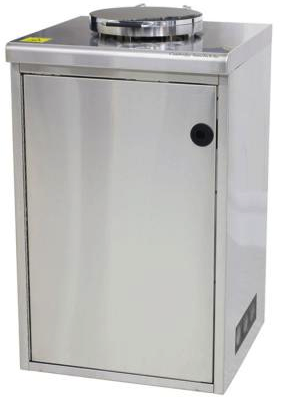
\includegraphics[height=8cm]{./Figures/Appendix/ALD-schematic/savannah-s100}%
	} 
	\hspace{1cm}
  \subfloat[Schematic Diagram][Schematic Diagram]{%
   	\label{fig:S100-schematic}%
	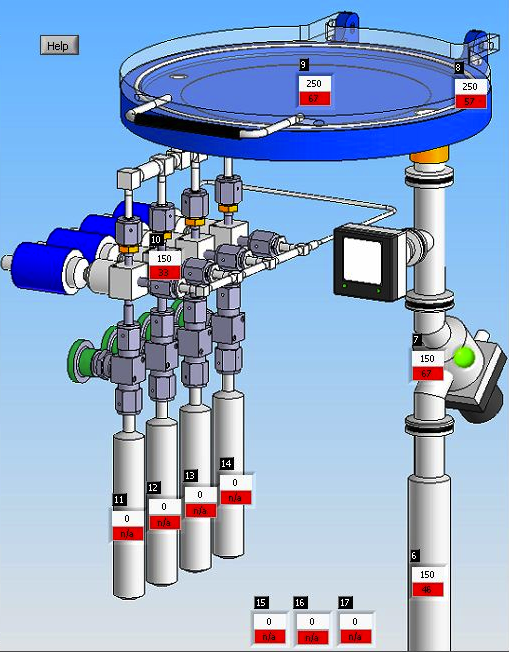
\includegraphics[height=8cm]{./Figures/Appendix/ALD-schematic/savannah-schematic}%
	} 	
   \caption[Cambridge NanoTech, inc. S100 ALD System]%
   		{Cambridge NanoTech, inc. Savannah S100 ALD reactor. Precursors are stored in heated cylinders, flow up to the reaction zone, and byproducts are pumped out of the vacuum line on the right side. Each zone can be individually temperature controlled.}
   \label{fig:S100}
\end{figure}

\clearpage
%
%\begin{figure}[htbp]
%	\begin{center}
%		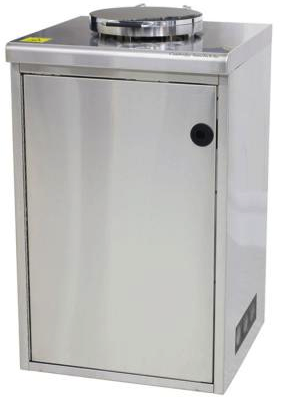
\includegraphics[width=0.5\textwidth]{./Figures/Appendix/ALD-schematic/savannah-s100}
%		\caption[Photograph of S100 ALD Reactor]{Photograph of the Cambridge NanoTech, inc. %
%				Savannah S100 ALD reactor}
%		\label{fig:S100-photo}
%	\end{center}
%\end{figure}
%
%\begin{figure}[htbp]
%	\begin{center}
%		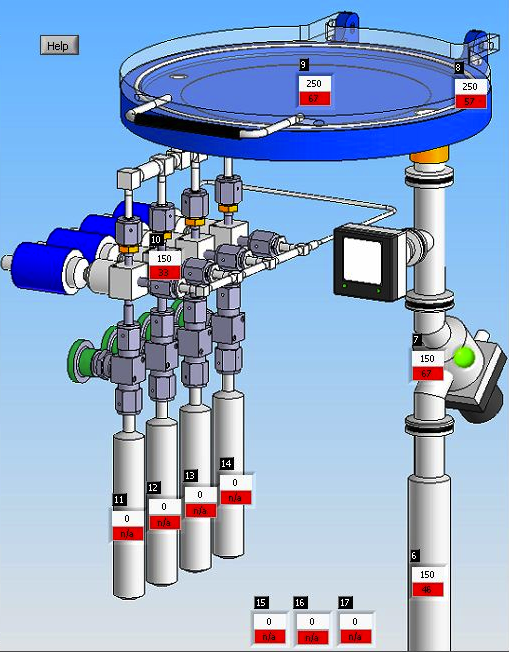
\includegraphics[width=0.85\textwidth]{./Figures/Appendix/ALD-schematic/savannah-schematic}
%		\caption[Diagram of S100 ALD Reactor]{Diagram of the Cambridge NanoTech, inc. %
%				Savannah S100 ALD reactor. Precursors are stored in heated cylinders, flow up to the reaction zone, and byproducts are pumped out of the vacuum line on the right side. Each zone can be individually temperature controlled. }
%		\label{fig:S100-schematic}
%	\end{center}
%\end{figure}


%\end{landscape}
%%%%%%%%%%%%%%%%%%%%%%%%%%%%%%%%%%%%%%%%%%%%%%%%%%%%
%%%%%%%%%%%%%%%%%%%%%%%%%%%%%%%%%%%%%%%%%%%%%%%%%%%%
%%%%%%%%%%%%%%%%%%%%%%%%%%%%%%%%%%%%%%%%%%%%%%%%%%%%

%\section{Recipes for S100 ALD System}
%\label{sup:recipes}
%
%Should recipes be provided? They'd be rather specific to the instrumentation, and some of the recipes are provided by CNT (able to freely publish them?). This section would be trivial to construct, or remove entirely. 
%%
%%Provided in this section are recipes for the deposition of materials in the \ce{Pb_{x}Ti_{y}O_{z}} system. 
%%Some of these recipes (\ce{HfO2}, \ce{Pt}, and \ce{TiO2}) were provided courtesy of Cambridge NanoTech, inc.\cite{CNT-web} 
%%
%\clearpage
%%%%%%%%%%%%%%%%%%%%%%%%%%%%%%%%%%%%%%%%%%%%%%%%%%%%
%%%%%%%%%%%%%%%%%%%%%%%%%%%%%%%%%%%%%%%%%%%%%%%%%%%%
%%%%%%%%%%%%%%%%%%%%%%%%%%%%%%%%%%%%%%%%%%%%%%%%%%%%

%\section{Thermal Analysis Results}
%\label{sup:Thermal-Results}
%
%\subsection{Thermogravimetric Analysis}
%\label{sup:Thermal-Results-TGA}
%
%%\begin{figure}[htbp]
%%   \centering
%%   \subfloat[Mass vs. Temperature][Mass vs. Temperature]{%
%%   	\label{fig:TGA-HFAc-Weight}%
%%	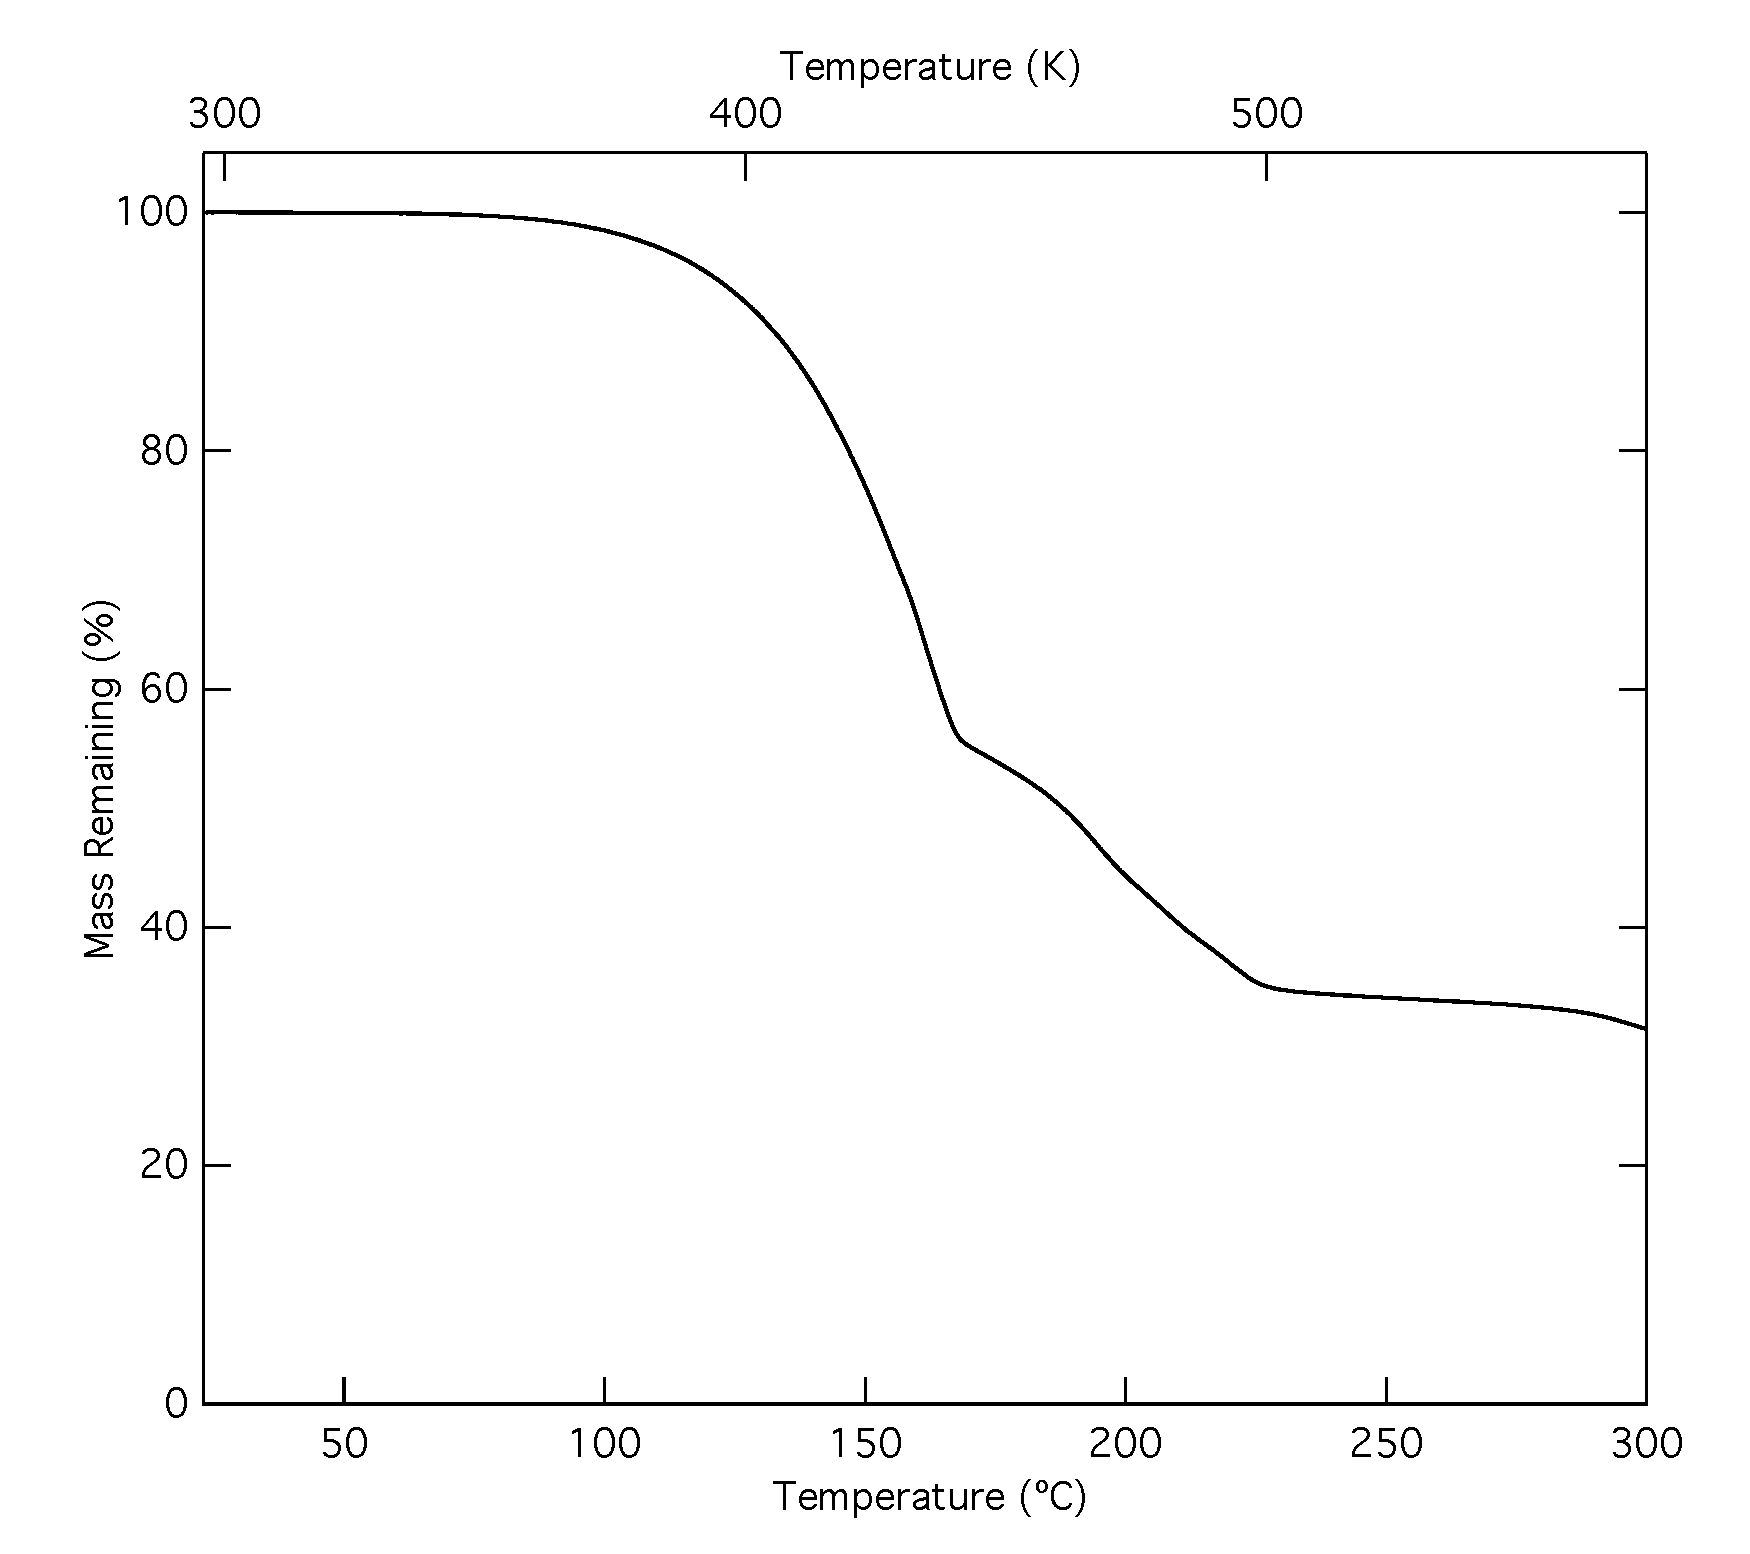
\includegraphics[width=0.5\textwidth]{./Figures/Appendix/Thermal-Analysis/TGA/HFAc-Weight}%
%%	} \\
%%%	\hspace{1cm}
%%  \subfloat[Derivative of Mass vs. Temperature][Derivative of Mass vs. Temperature]{%
%%   	\label{fig:TGA-HFAc-DWeight}%
%%	\includegraphics[width=0.5\textwidth]{./Figures/Appendix/Thermal-Analysis/TGA/HFAc-DWeight}%
%%	} 	
%%   \caption[TGA Results for Pb(HFAc)$_{2}$ Precursor]%
%%   		{Plots of the results from TGA experiments on Pb(HFAc)$_{2}$. The plot shown in (a) gives the raw %
%%		data showing the current mass as a function of temperature. (b) gives the same data, transformed %
%%		to show the derivative of mass. Thus (b) shows the rate of mass loss at a given temperature. Initial %
%%		sample mass: 6.092 mg}
%%   \label{fig:TGA-HFAc}
%%\end{figure}
%%
%%\begin{figure}[htbp]
%%   \centering
%%   \subfloat[Mass vs. Temperature][Mass vs. Temperature]{%
%%   	\label{fig:TGA-TMHD-Weight}%
%%	\includegraphics[width=0.75\textwidth]{./Figures/Appendix/Thermal-Analysis/TGA/TMHD-Weight}%
%%	} \\
%%%	\hspace{1cm}
%%  \subfloat[Derivative of Mass vs. Temperature][Derivative of Mass vs. Temperature]{%
%%   	\label{fig:TGA-TMHD-DWeight}%
%%	\includegraphics[width=0.75\textwidth]{./Figures/Appendix/Thermal-Analysis/TGA/TMHD-DWeight}%
%%	} 	
%%   \caption[TGA Results for Pb(HFAc)$_{2}$ Precursor]%
%%   		{Plots of the results from TGA experiments on Pb(TMHD)$_{2}$. As in figure~\vref{fig:TGA-HFAc}, (a) %
%%		presents the actual mass as a function of temperature, while (b) gives the derivative of that function. %
%%		Initial sample mass: 3.719 mg}
%%   \label{fig:TGA-TMHD}
%%\end{figure}
%
%
%%\begin{figure}[htbp]
%%   \centering
%%   \subfloat[\HFAc][\HFAc]{%
%%   	\label{fig:TGA-HFAc-Hold}%
%%	\includegraphics[width=0.75\textwidth]{./Figures/Appendix/Thermal-Analysis/TGA/HFAc-Hold}%
%%	} \\
%%%	\hspace{1cm}
%%  \subfloat[\TMHD][\TMHD]{%
%%   	\label{fig:TGA-TMHD-Hold}%
%%	\includegraphics[width=0.75\textwidth]{./Figures/Appendix/Thermal-Analysis/TGA/TMHD-Hold}%
%%	} 	
%%   \caption[Constant Temperature TGA Experiments]%
%%   		{Plots of the results from ramp-and-hold TGA experiments designed to investigate residual material %
%%		after complete evaporation at a given temperature. From the TGA experiments seen above (figs.~%
%%		\vref{fig:TGA-HFAc} and \vref{fig:TGA-TMHD}), a common temperature of 160\degC{} was chosen %
%%		for this experiment. Sample sizes were 3.921 mg and 4.381 mg for \HFAc{} and \TMHD{} respectively.}
%%   \label{fig:TGA-Hold}
%%\end{figure}
%
%\clearpage
%
%%%%%%%%%%%%%%%%%%%%%%%%%%%%%

%\subsection{Differential Scanning Calorimetry}
%\label{sup:Thermal-Results-DSC}

%\begin{figure}[htbp]
%   \centering
%   \subfloat[Pb(HFAc)$_{2}$][Pb(HFAc)$_{2}$]{%
%   	\label{fig:DSC-HFAc}%
%	\includegraphics[width=0.75\textwidth]{./Figures/Appendix/Thermal-Analysis/DSC/HFAc}%
%	} \\
%  \subfloat[Pb(TMHD)$_{2}$][Pb(TMHD)$_{2}$]{%
%   	\label{fig:DSC-TMHD}%
%	\includegraphics[width=0.75\textwidth]{./Figures/Appendix/Thermal-Analysis/DSC/TMHD}%
%	} 	
%   \caption[Results of DSC Experiments]%
%   		{This plot shows results from DSC experiments carried out during the course of %
%		this project. (a) shows the results from analyzing the Pb(HFAC)$_{2}$ compound. (b) gives %
%		the data from Pb(TMHD)$_{2}$. Exothermic (heat release) flow is positive in both plots. }
%   \label{fig:DSC-Data}
%\end{figure}

%\clearpage

%\begin{figure}[htbp]
%	\begin{center}
%		\includegraphics[width=0.75\textwidth]{./Figures/Appendix/Thermal-Analysis/DSC/HFAc}
%		\caption[DSC of Pb(HFAc)$_{2}$]{This plot shows the result of a DSC experiment on the %
%				Pb(HFAc)$_{2}$ precursor. It shows the major points where energy is absorbed or %
%				released, and analysis of these points can give significant information about the %
%				thermal behavior and the transition mechanisms.}
%		\label{fig:DSC-HFAc}
%	\end{center}
%\end{figure}
%
%\begin{figure}[htbp]
%	\begin{center}
%		\includegraphics[width=0.75\textwidth]{./Figures/Appendix/Thermal-Analysis/DSC/TMHD}
%		\caption[DSC of Pb(TMHD)$_{2}$]{This plot shows the result of a DSC experiment on the %
%				Pb(TMHD)$_{2}$ precursor. As in figure~\vref{fig:DSC-HFAc}, analysis of this plot %
%				can give meaningful information on what is chemically happening to the %
%				compound as the temperature changes.}
%		\label{fig:DSC-TMHD}
%	\end{center}
%\end{figure}

%%%%%%%%%%%%%%%%%%%%%%%%%%%%%%%%%%%%%%%%%%%%%%%%%%%%
%%%%%%%%%%%%%%%%%%%%%%%%%%%%%%%%%%%%%%%%%%%%%%%%%%%%
%%%%%%%%%%%%%%%%%%%%%%%%%%%%%%%%%%%%%%%%%%%%%%%%%%%%

\section{Composition Results}
\label{sup:Composition}

%\begin{table}[htbp]
%	\centering
%	\caption[XRF Calculated Compositions]{Calculated compositions of selected samples, determined via XRF. \\Composition percentages are all $\pm$1\%.\label{tbl:XRF-compositions}}
%	\begin{tabular}{l l r r r}
%	\toprule
%	&&\multicolumn{3}{c}{Composition (\%)}\\
%	\cmidrule{3-5}
%	Run \#&Substrate&Lead&Titanium&Ti:Pb Ratio\\
%	\midrule
%% 	Run	Sub-Type		Pb%		Ti%		Ti:Pb ratio
%	0	&\ce{SiO2}	&55.99	&44.01	&0.786\\
%	1	&\ce{SiO2}	&55.00	&45.00	&0.809\\
%	13	&\ce{SiO2}	&53.96	&46.04	&0.853\\
%	16	&\ce{SiO2}	&49.45	&50.55	&1.022\\
%	19	&\ce{SiO2}	&65.87	&34.13	&0.518\\
%		&Pt-Si		&42.86	&57.14	&1.333\\
%	20	&\ce{SiO2}	&56.52	&43.48	&0.769\\
%		&\ce{Pt-Si}	&51.43	&48.57	&0.944\\
%	21	&\ce{SiO2}	&69.60	&30.40	&0.437\\
%		&Pt-Si		&56.08	&43.92	&0.783\\
%	22	&\ce{SiO2}	&67.64	&32.36	&0.478\\
%		&Pt-Si		&56.06	&43.94	&0.784\\
%	23	&\ce{SiO2}	&66.89	&33.11	&0.495\\
%		&Pt-Si		&49.06	&50.94	&1.038\\
%	24	&\ce{SiO2}	&68.96	&31.06	&0.450\\
%		&Pt-Si		&62.16	&37.84	&0.609\\
%	\bottomrule
%	\end{tabular}
%\end{table}

\begin{figure}[htbp]
	\centering
	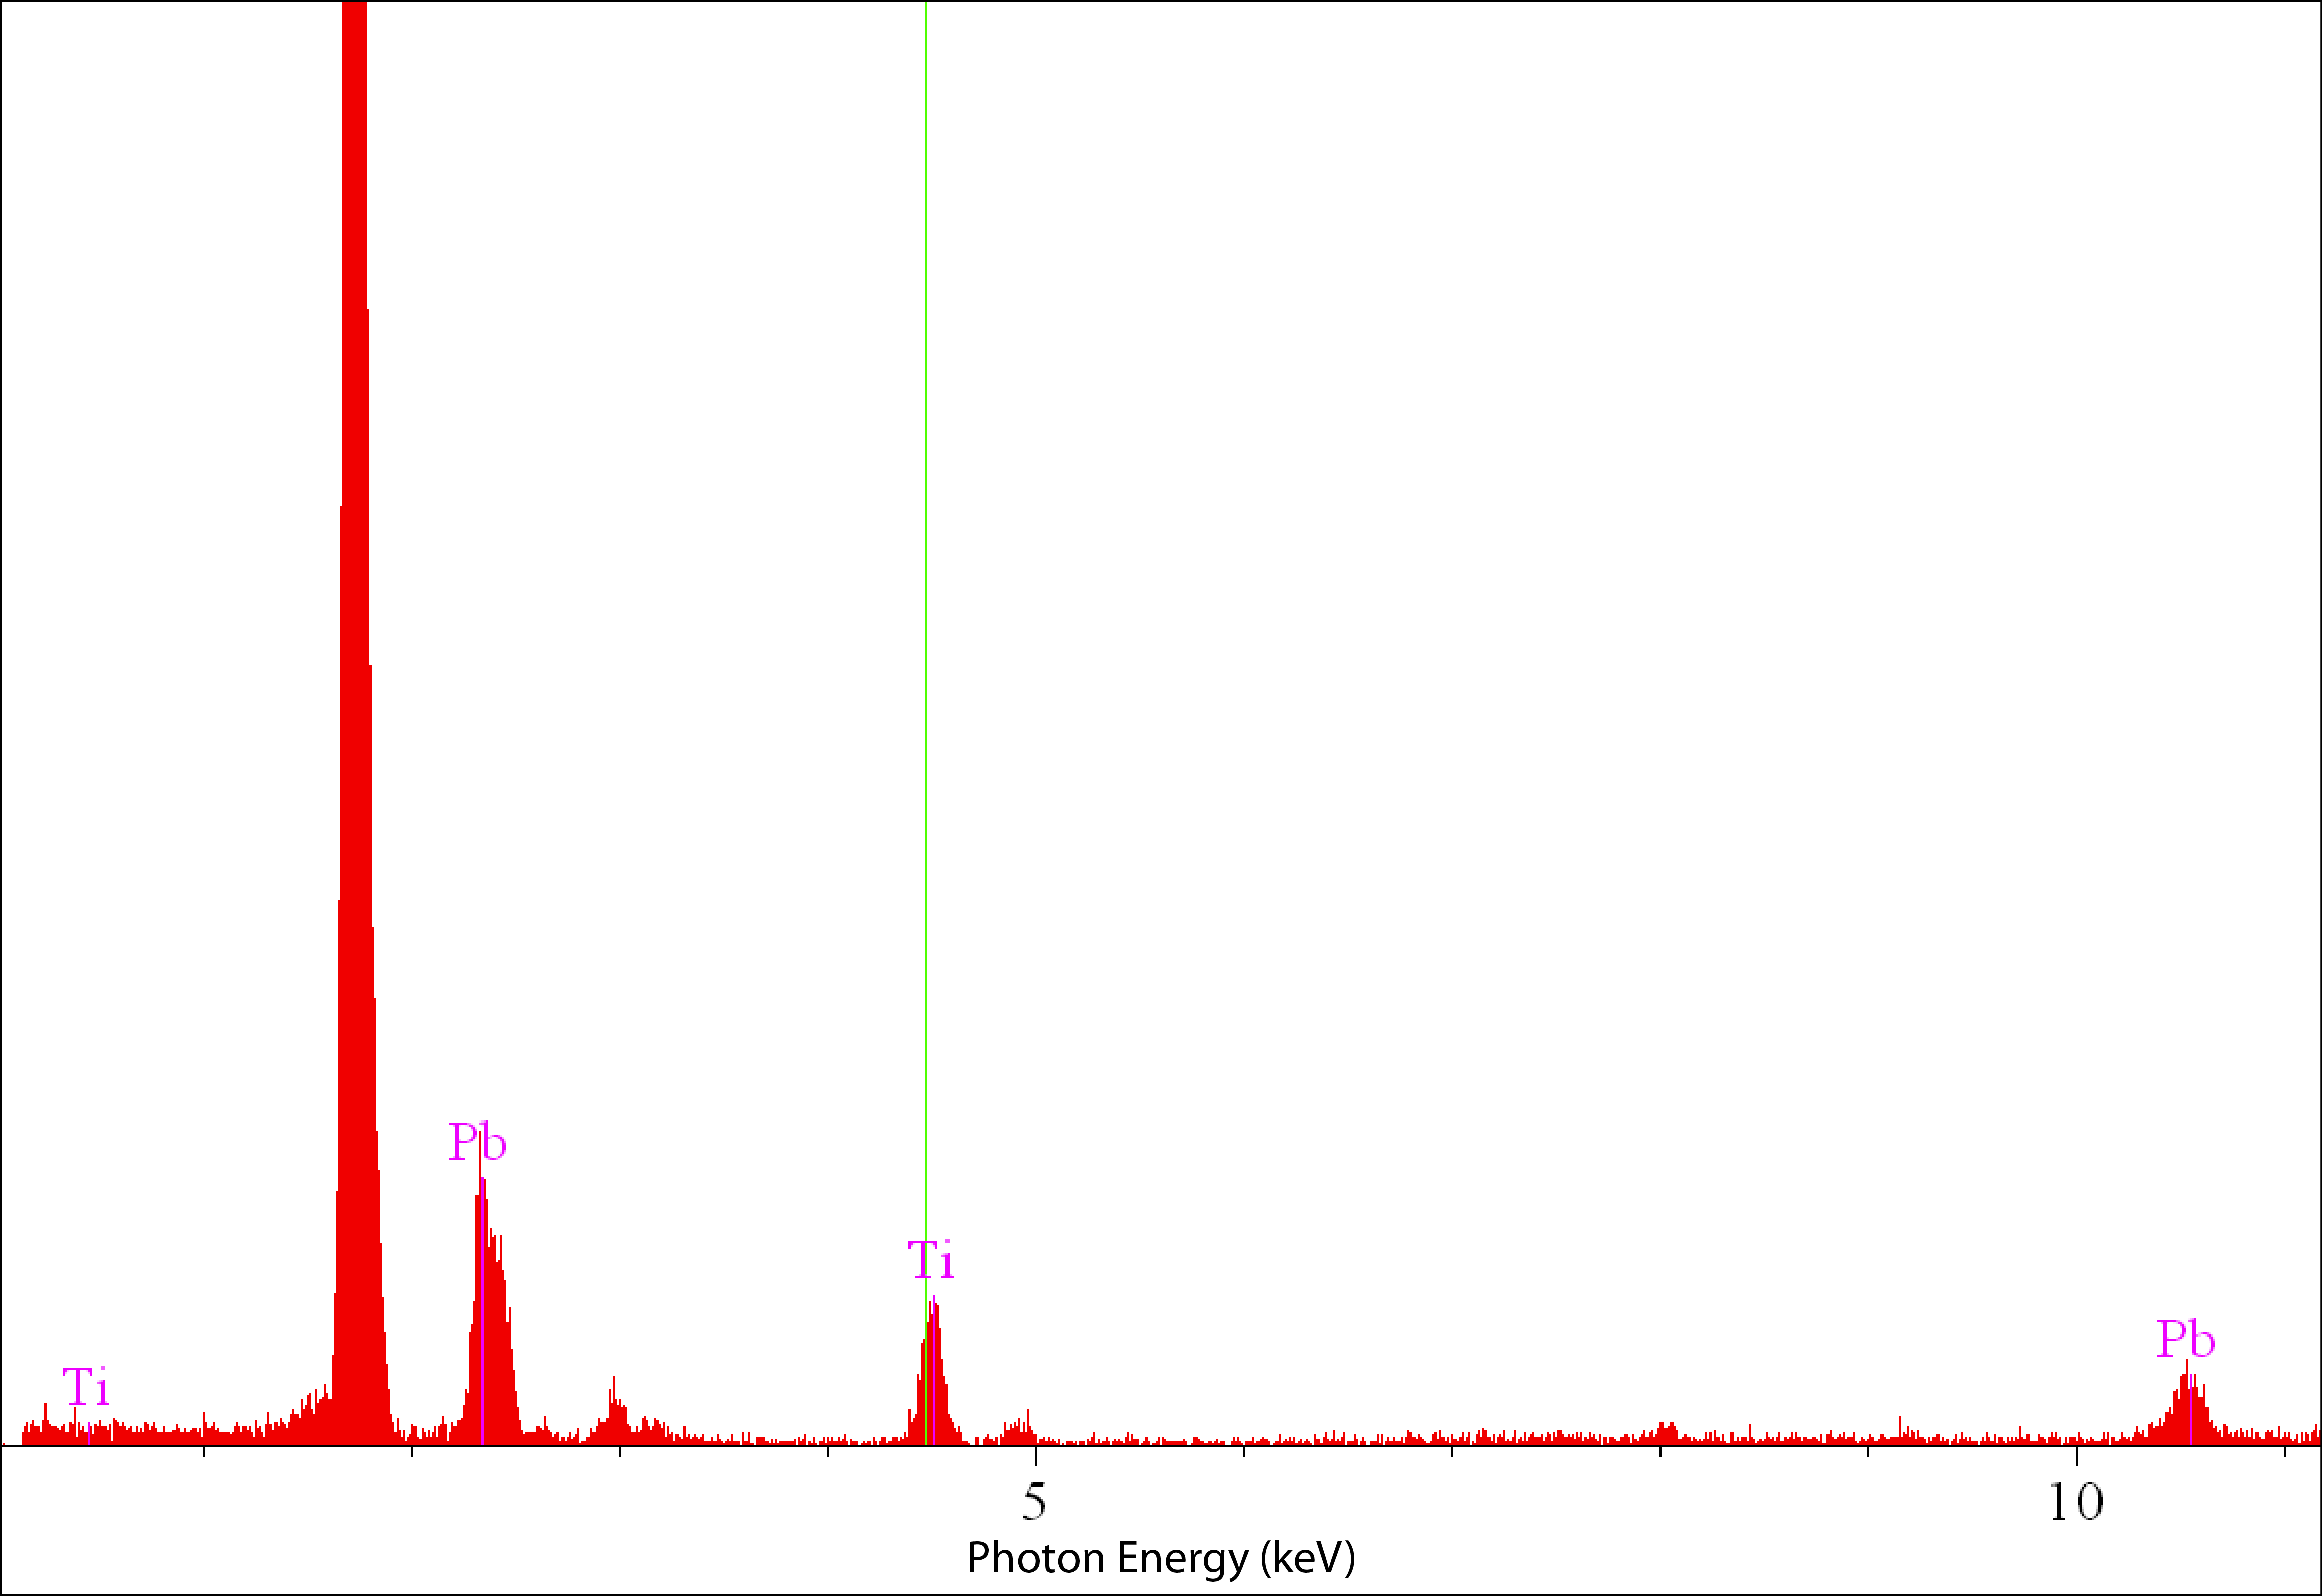
\includegraphics[width=0.85\textwidth]{./Figures/Appendix/Composition/PTO-run0-pre-anneal.png}
	\caption[XRF Spectrum of PTO \#0]%
		     {The XRF spectrum collected from deposition run \#0.  }
	\label{fig:XRF-0-SiO2}
\end{figure}

\begin{figure}[htbp]
	\centering
	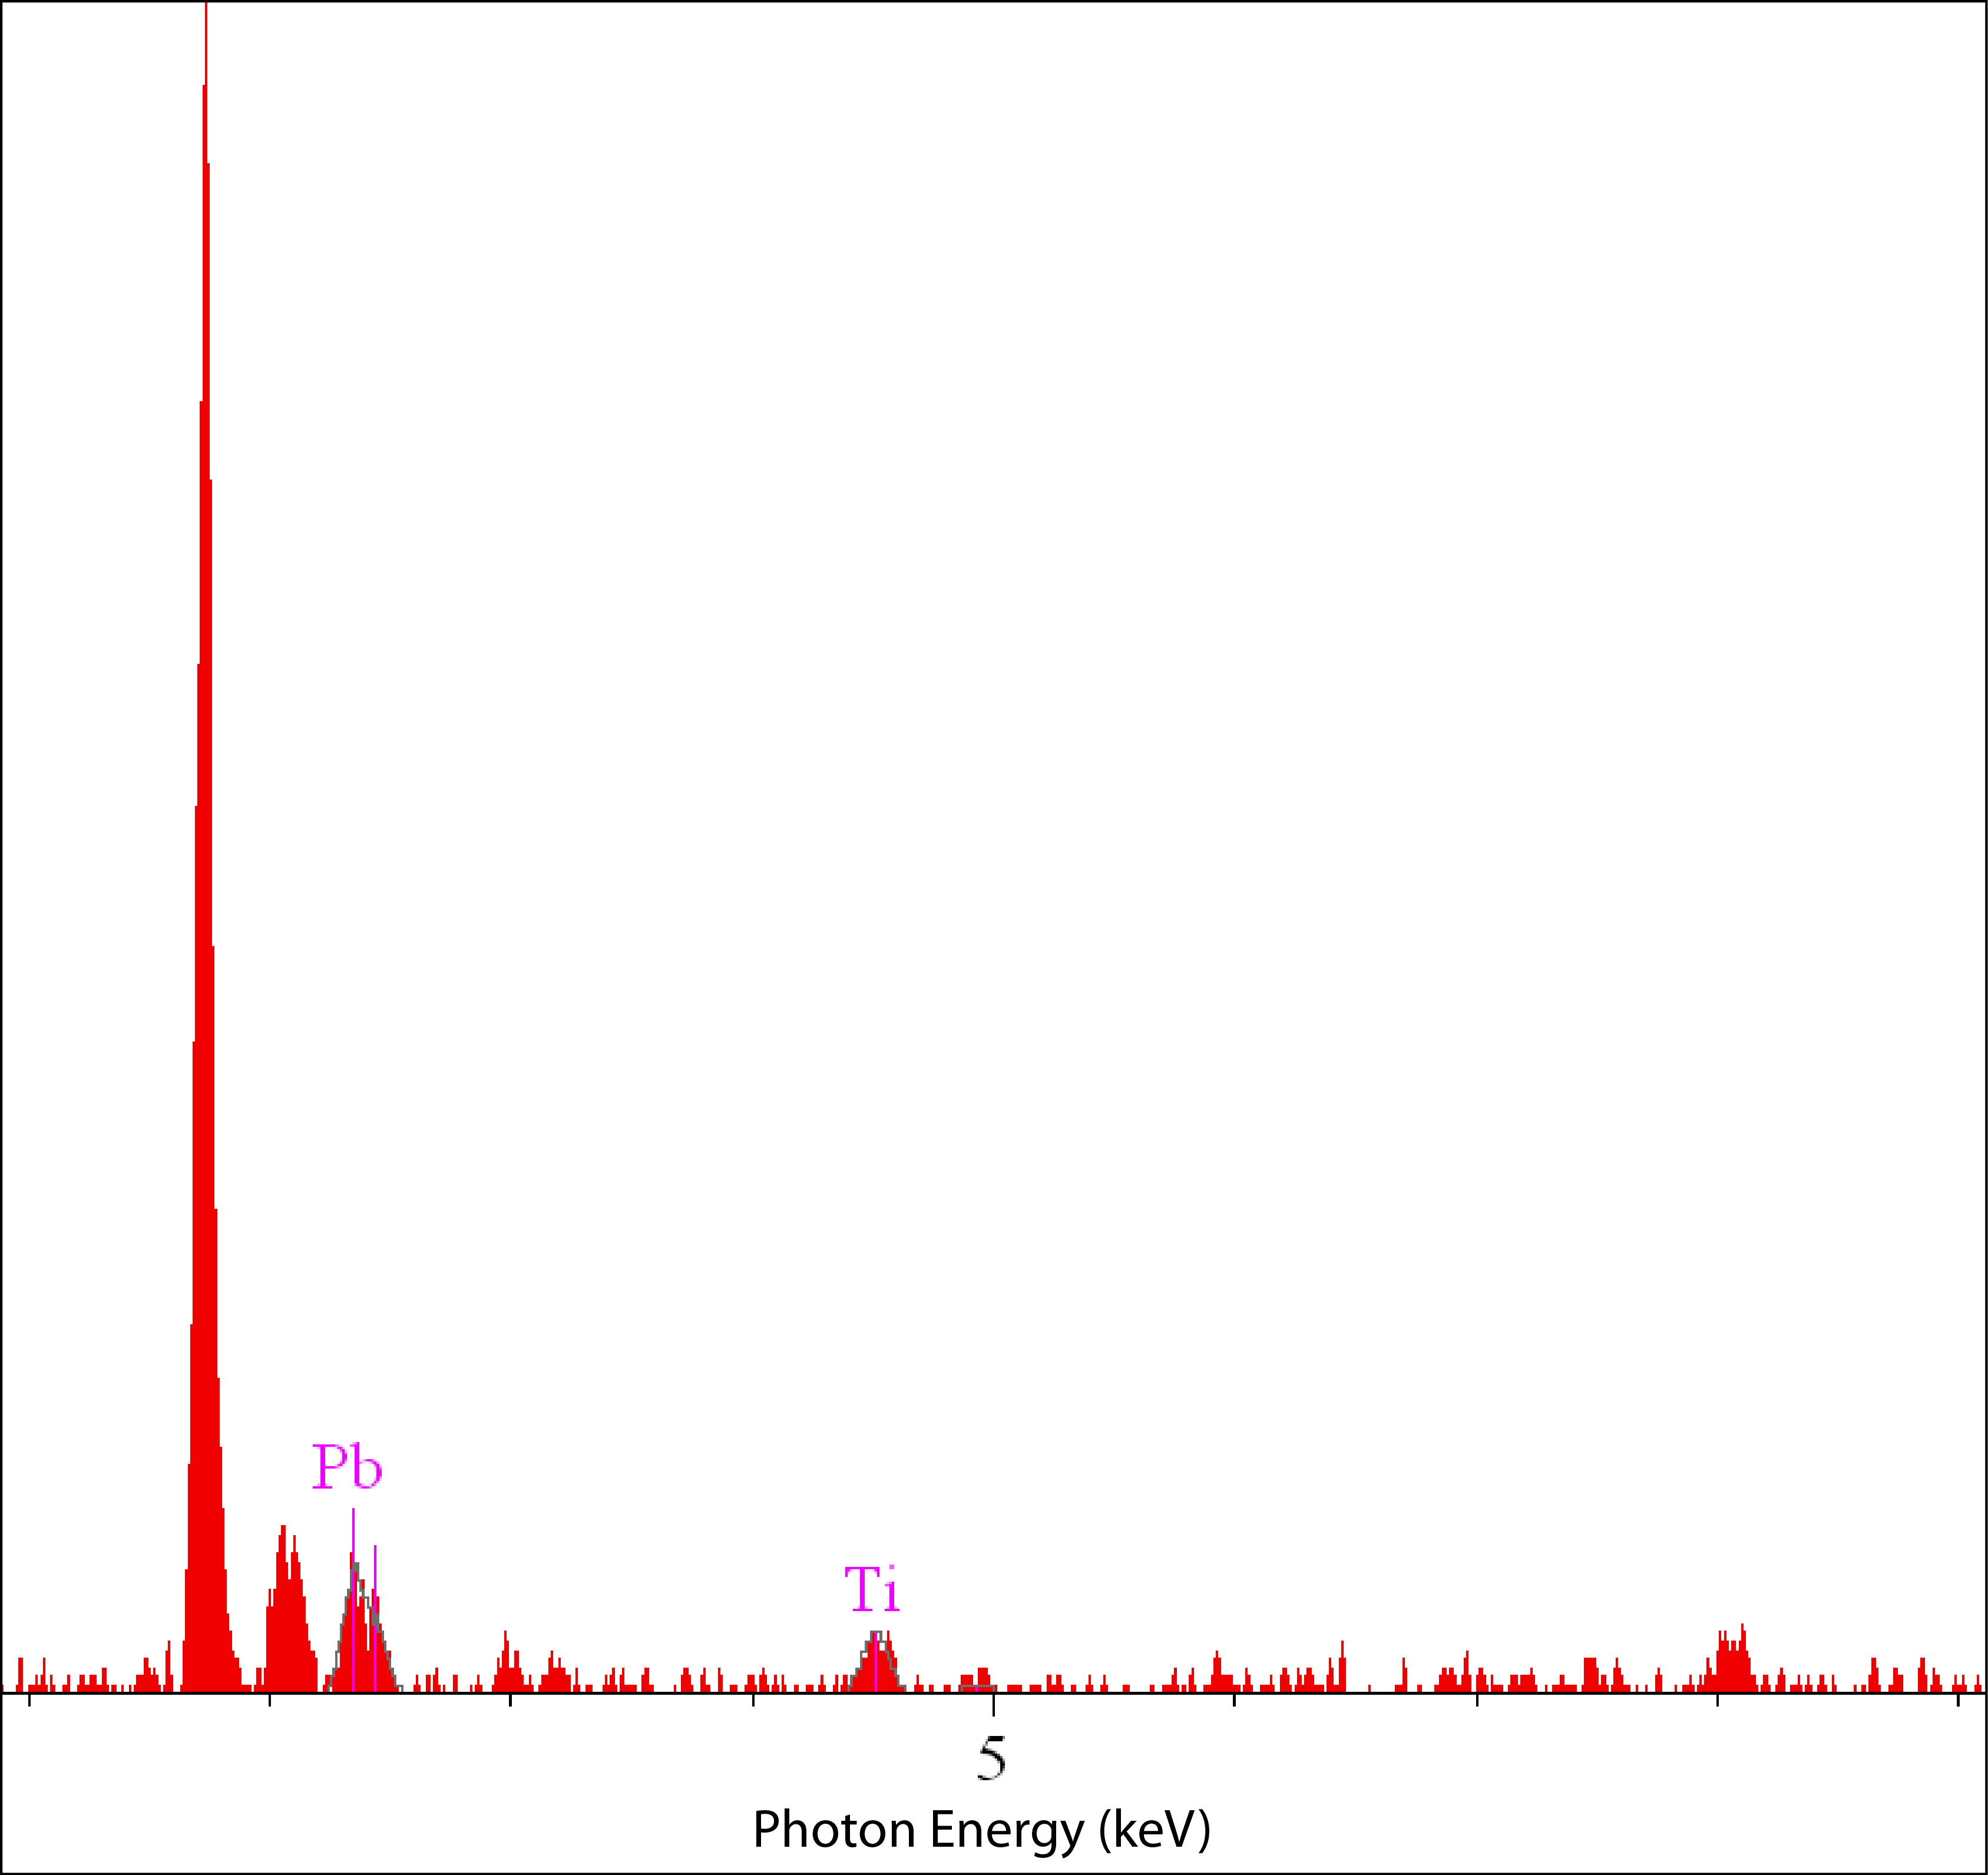
\includegraphics[width=0.85\textwidth]{./Figures/Appendix/Composition/PTO-run20-pt.png}
	\caption[XRF Spectrum of PTO \#20 on Pt-Si]%
		     {The XRF spectrum collected from deposition run \#20 deposited on platinized silicon. The peak between the substrate and Pb is that of Pt. }
	\label{fig:XRF-20-Pt}
\end{figure}

\clearpage
%%%%%%%%%%%%%%%%%%%%%%%%%%%%%%%%%%%%%%%%%%%%%%%%%%%%
%%%%%%%%%%%%%%%%%%%%%%%%%%%%%%%%%%%%%%%%%%%%%%%%%%%%
%%%%%%%%%%%%%%%%%%%%%%%%%%%%%%%%%%%%%%%%%%%%%%%%%%%%

\section{Ellipsometry Results}
\label{sup:Ellipsometry}

\begin{table}[htbp]
	\centering
	\caption[PTO \#0 Ellipsometric Model Variables]{Variables used to produce the\\model fit for PTO \#0 seen in fig.~\vref{fig:Ellip-0-SiO2}. \label{tbl:PTO-0-ellip-variables}}
	\begin{tabular}{l l r r}
	\toprule
	Layer&Variable&Thickness (nm)&Value\\
	\midrule
	2. T-L Osc.&&88.7&\\
	&$\epsilon_{1}$ offset&&2.49\\
	&Amp&&12.66\\
	&E$_{\mathrm{n}}$&&4.60\\
	&C&&1.35\\
	&E$_{\mathrm{g}}$&&0.86\\
	1. \ce{SiO2}&&203.7&\\
	0. \ce{Si}&&Substrate&\\
	\bottomrule
	\end{tabular}
\end{table}

\begin{figure}[htbp]
   \centering
   \subfloat[Psi vs. Wavelength][Psi ($\Psi$) vs. Wavelength ($\lambda$)]{%
   	\label{fig:Ellip-0-SiO2-Psi}%
	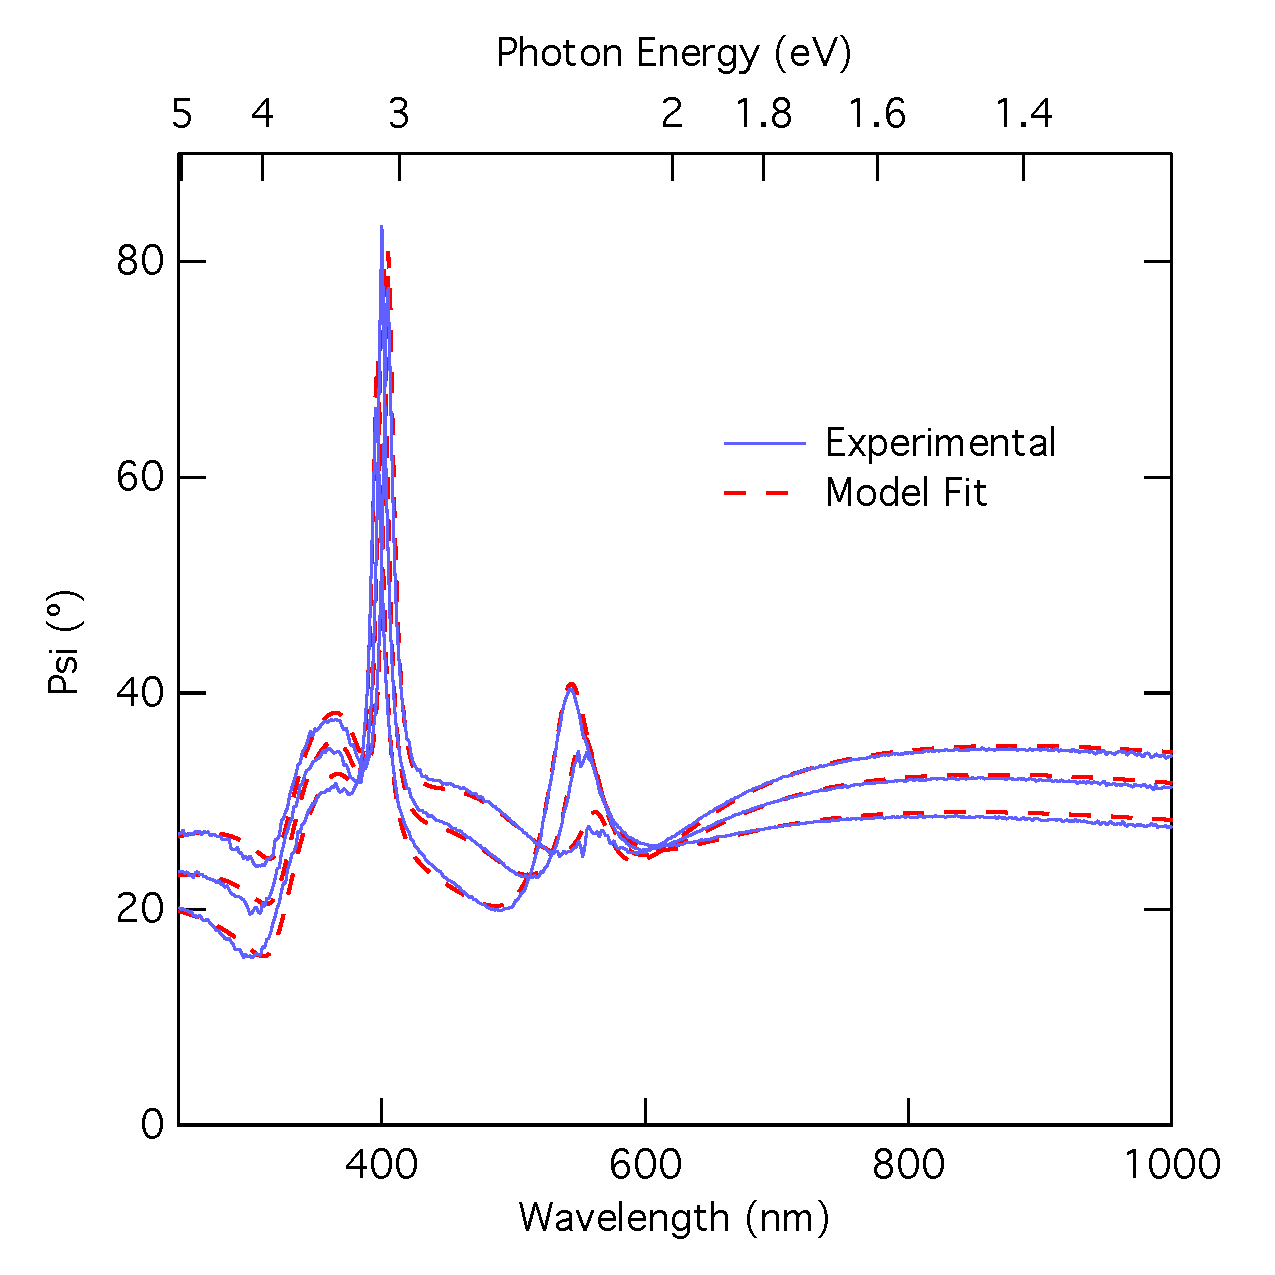
\includegraphics[width=0.47\textwidth]{./Figures/Appendix/Ellipsometry/Run-0-SiO2/Psi.pdf}%
	}\hspace{0.5cm}
  \subfloat[Delta vs. Wavelength][Delta ($\Delta$) vs. Wavelength ($\lambda$)]{%
   	\label{fig:Ellip-0-SiO2-Delta}%
	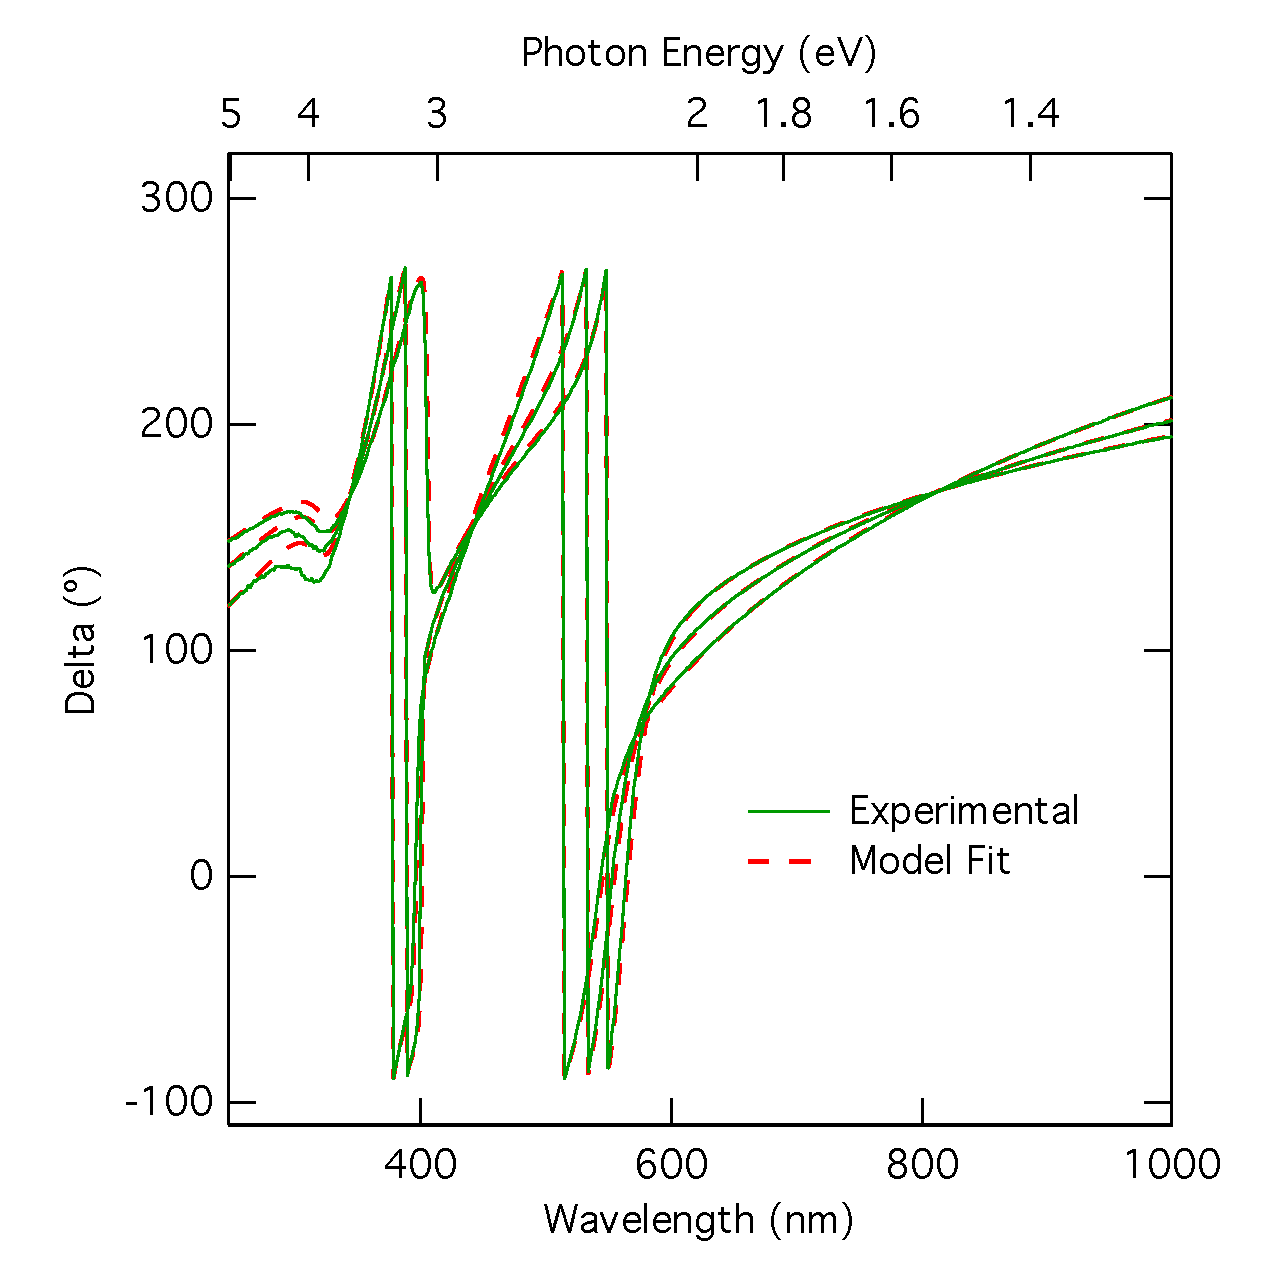
\includegraphics[width=0.47\textwidth]{./Figures/Appendix/Ellipsometry/Run-0-SiO2/Delta.pdf}%
	} \\
  \subfloat[$n$, $k$ vs. Photon Energy][$n$, $k$ vs. Photon Energy (eV)]{%
   	\label{fig:Ellip-0-SiO2-nk}%
	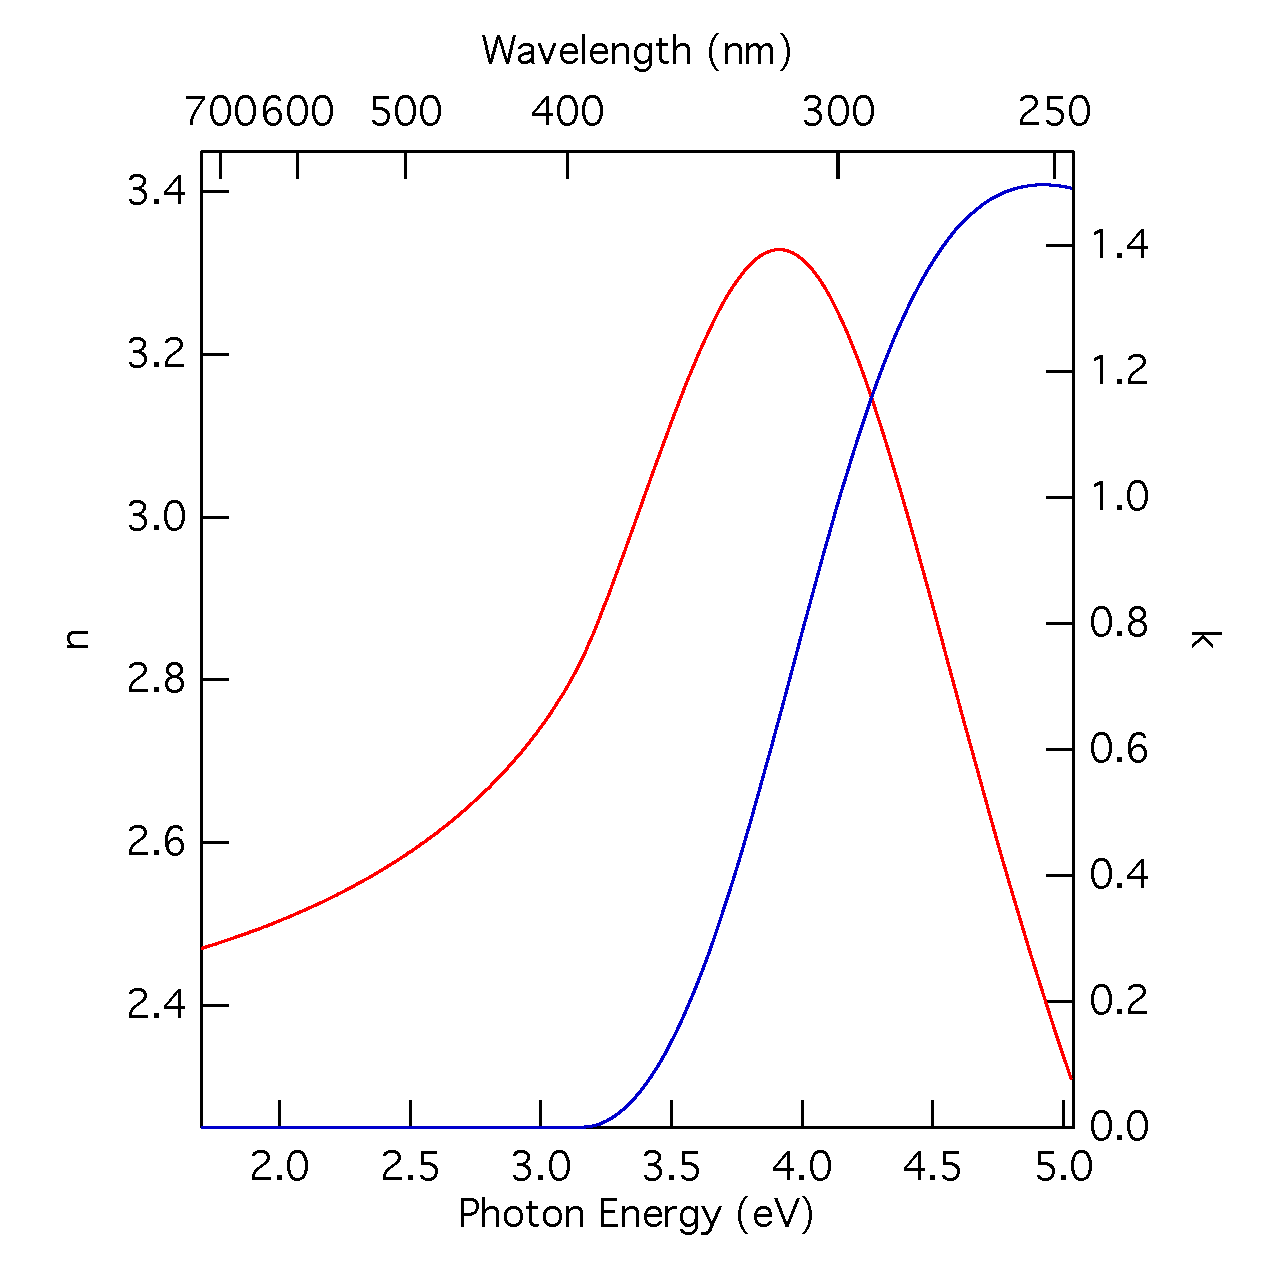
\includegraphics[width=0.47\textwidth]{./Figures/Appendix/Ellipsometry/Run-0-SiO2/n,k.pdf}%
	}
   \caption[Results of Ellipsometry on Sample \#0]%
   		{The set of plots shown above show the results from ellipsometric analysis on sample \#0 (see %
		table~\vref{tbl:LoSamples}) grown on a silicon wafer and subsequently annealed. (a) and (b) %
		show the data and the modeled fit from the experiment. (c) shows the components of the complex %
		index of refraction ($\tilde n$), $n$ and $k$. Band gap estimation was performed using the values %
		of $k$. The highlighted portion of $k$ is the nearly linear region used in this analysis.}
   \label{fig:Ellip-0-SiO2}
\end{figure}

\begin{figure}[htbp]
   \centering
   \subfloat[Absorption ($\alpha$) vs. Photon Energy][Absorption ($\alpha$) vs. Photon Energy (eV)]{%
   	\label{fig:Ellip-0-SiO2-alpha}%
	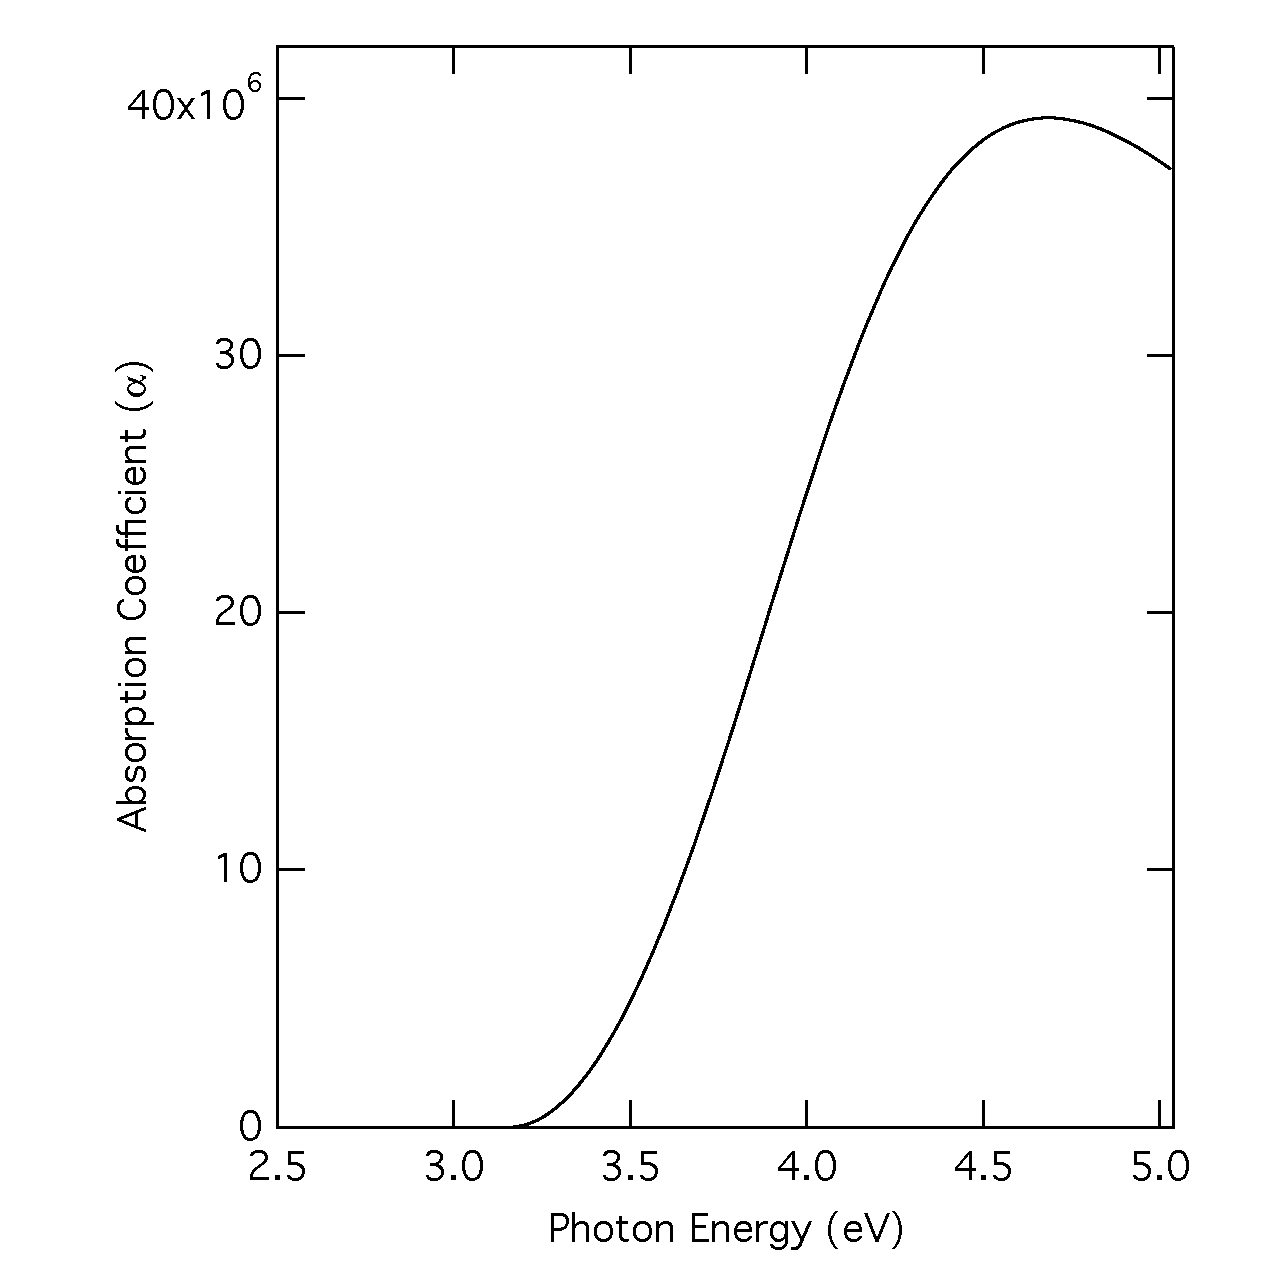
\includegraphics[width=0.47\textwidth]{./Figures/Appendix/Ellipsometry/Run-0-SiO2/alpha.pdf}%
	}\hspace{0.5cm}
  \subfloat[Tauc ($\alpha^{2}E_{ph}^{2}$) vs. Photon Energy][Tauc ($\alpha^{2}E_{ph}^{2}$) vs. Photon Energy (eV)]{%
   	\label{fig:Ellip-0-SiO2-Tauc}%
	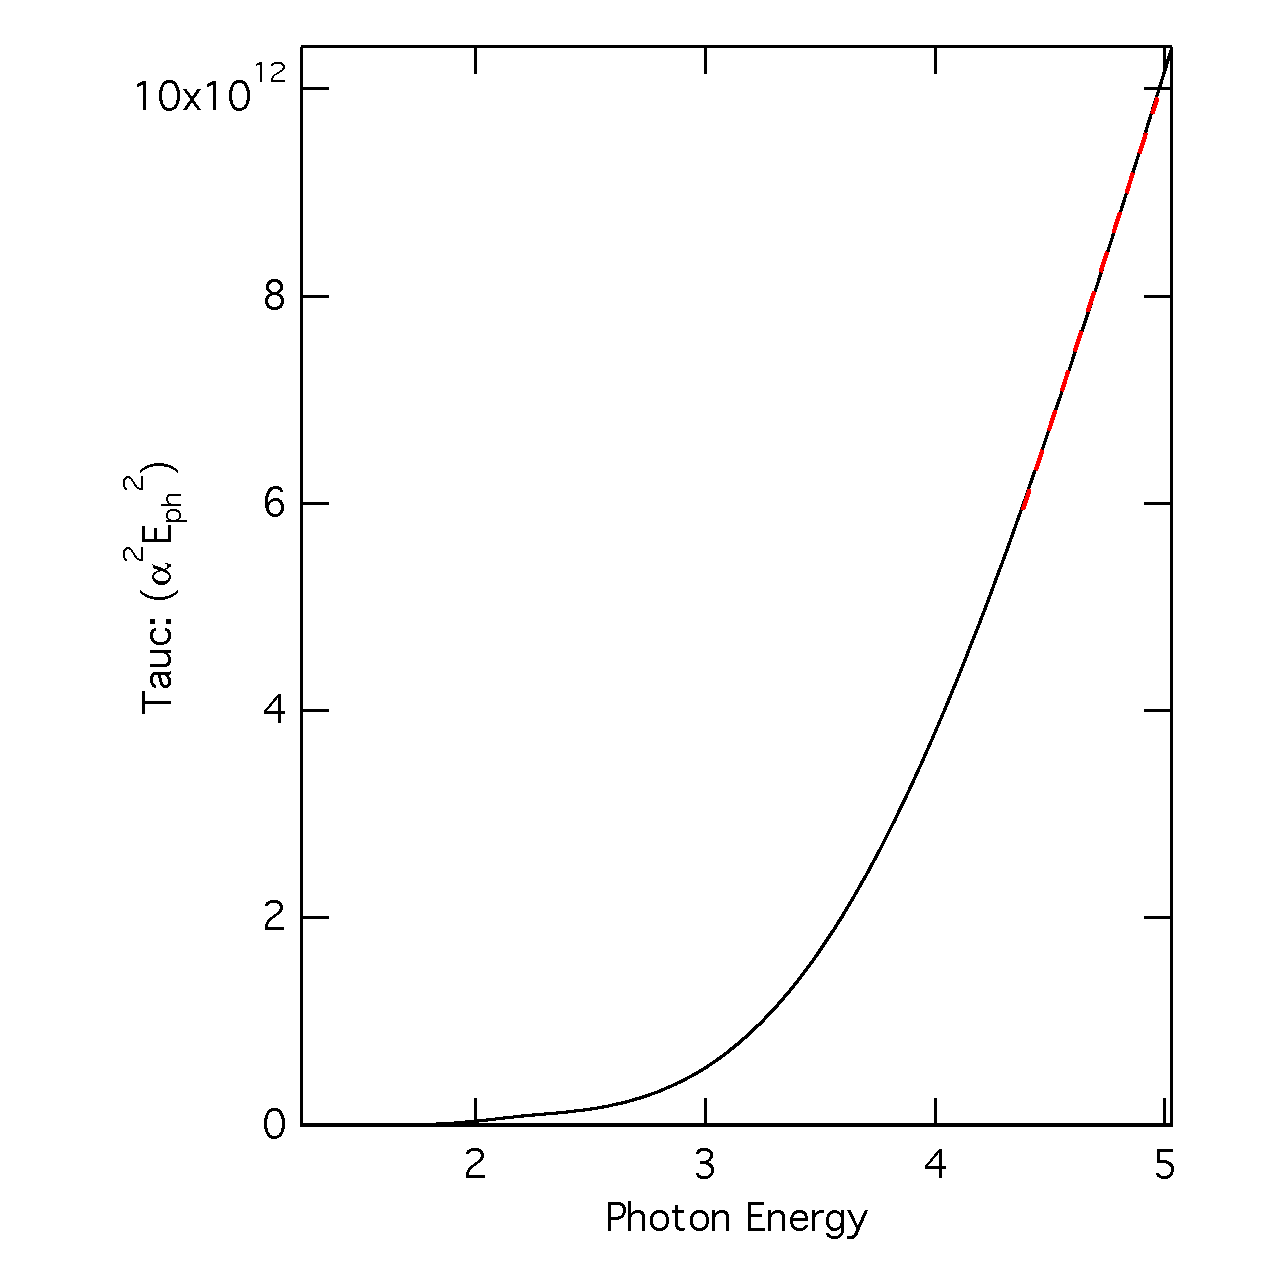
\includegraphics[width=0.47\textwidth]{./Figures/Appendix/Ellipsometry/Run-0-SiO2/tauc.pdf}%
	}
   \caption[Results of Tauc Analysis on Sample \#0]%
   		{Tauc analysis used to determine the bandgap of PTO \#0. (a) shows the %
		values of the absorption coefficient ($\alpha$) calculated from $k$ (seen in figure~%
		\vref{fig:Ellip-0-SiO2-nk}). (b) shows the Tauc plot, the linear region can provide an estimate of the %
		bandgap of the material. }
   \label{fig:Tauc-0-SiO2}
\end{figure}

\begin{table}[htbp]
	\centering
	\caption[PTO \#20 Ellipsometric Model Variables]{Variables used to produce the\\model fit for PTO \#20 seen in fig.~\vref{fig:Ellip-20-Pt}. \label{tbl:PTO-20-ellip-variables}}
	\begin{tabular}{l l r r}
	\toprule
	Layer&Variable&Thickness (nm)&Value\\
	\midrule
	3. T-L Osc.&&75.6&\\
	&$\epsilon_{1}$ offset&&3.62\\
	&Amp&&36.54\\
	&E$_{\mathrm{n}}$&&4.51\\
	&C&&1.30\\
	&E$_{\mathrm{g}}$&&2.07\\
	2. \ce{Pt}&&15.1&\\
	1. \ce{SiO2}&& 1.1\\
	0. \ce{Si}&&Substrate&\\
	\bottomrule
	\end{tabular}
\end{table}

\begin{figure}[htbp]
   \centering
   \subfloat[Psi vs. Wavelength][Psi ($\Psi$) vs. Wavelength ($\lambda$)]{%
   	\label{fig:Ellip-20-Pt-Psi}%
	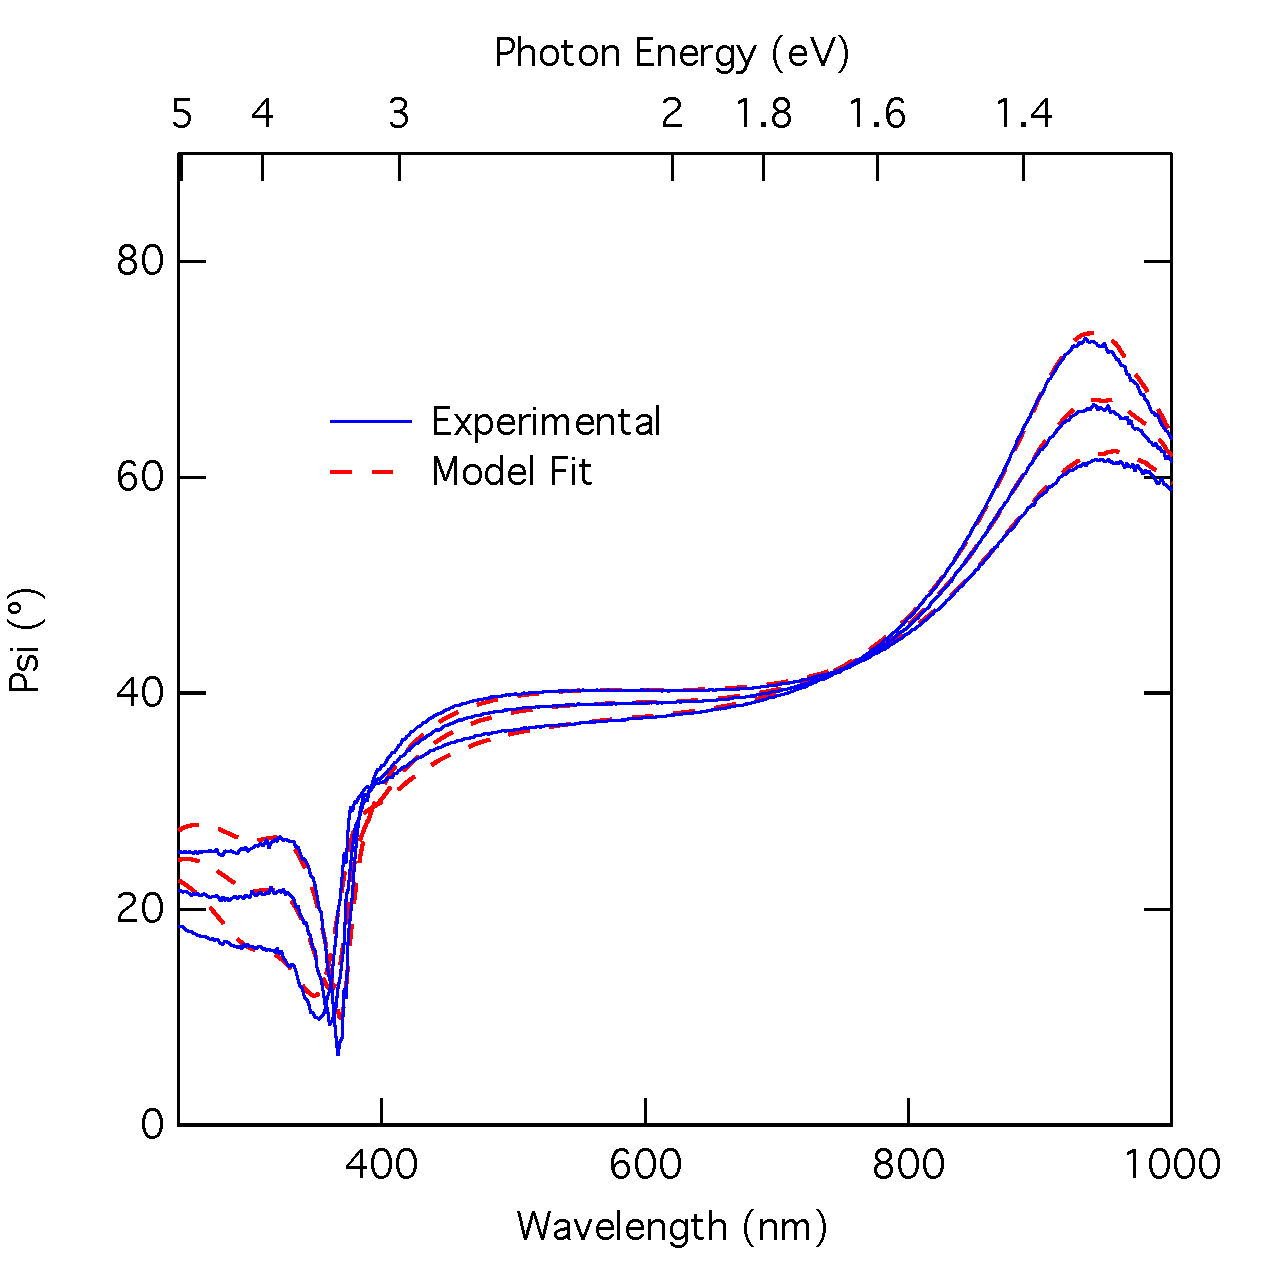
\includegraphics[width=0.47\textwidth]{./Figures/Appendix/Ellipsometry/Run-20-Pt/Psi.pdf}%
	}\hspace{0.5cm}
  \subfloat[Delta vs. Wavelength][Delta ($\Delta$) vs. Wavelength ($\lambda$)]{%
   	\label{fig:Ellip-20-Pt-Delta}%
	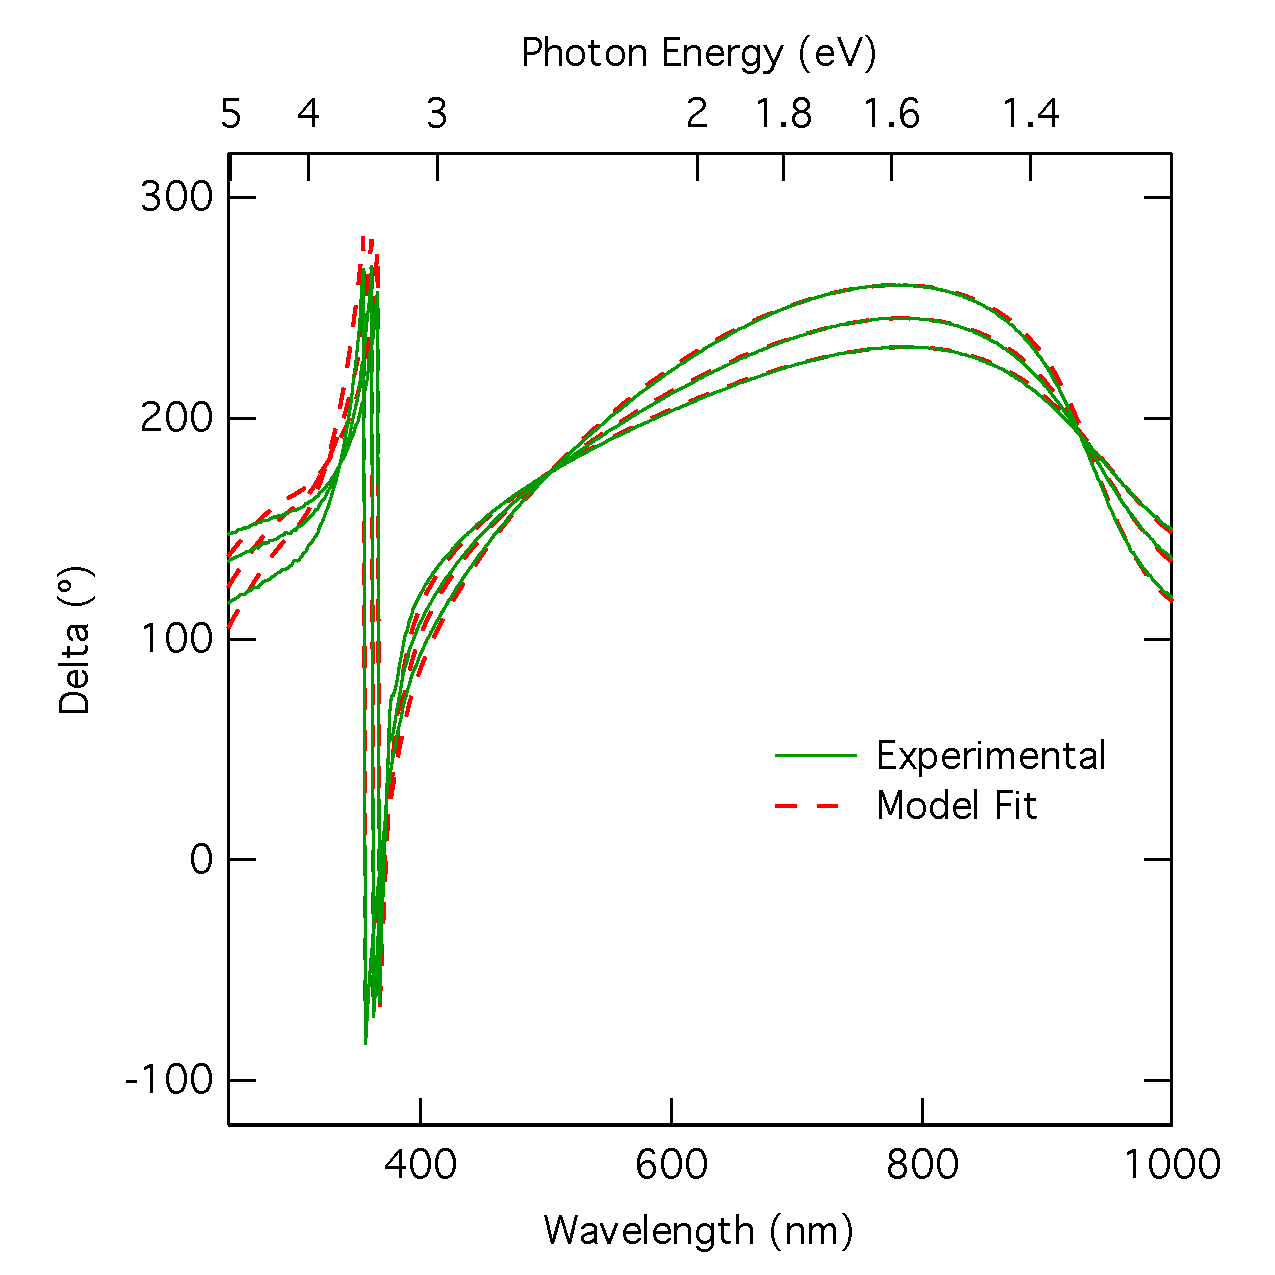
\includegraphics[width=0.47\textwidth]{./Figures/Appendix/Ellipsometry/Run-20-Pt/Delta.pdf}%
	} \\
  \subfloat[$n$, $k$ vs. Photon Energy][$n$, $k$ vs. Photon Energy (eV)]{%
   	\label{fig:Ellip-20-Pt-nk}%
	\includegraphics[width=0.47\textwidth]{./Figures/Appendix/Ellipsometry/Run-20-Pt/n,k.pdf}%
	}
   \caption[Results of Ellipsometry on Sample \#20 on Platinized Silicon]%
   		{Results of ellipsometric analysis on sample \#20, deposited on a platinized silicon substrate. As in fig.\ref{fig:Ellip-0-SiO2}, (a) and (b) show the experimental data and model fits of psi and delta (respectively). (c) gives the plot of calculated $n$ and $k$. For model parameters, see table~\vref{tbl:PTO-20-ellip-variables}}
		\label{fig:Ellip-20-Pt}
\end{figure}

\begin{figure}[htbp]
   \label{fig:Tauc-20-Pt}
   \centering
   \subfloat[Absorption ($\alpha$) vs. Photon Energy][Absorption ($\alpha$) vs. Photon Energy (eV)]{%
   	\label{fig:Ellip-20-Pt-alpha}%
	\includegraphics[width=0.47\textwidth]{./Figures/Appendix/Ellipsometry/Run-20-Pt/alpha.pdf}%
	}\hspace{0.5cm}
  \subfloat[Tauc ($\alpha^{2}E_{ph}^{2}$) vs. Photon Energy][Tauc ($\alpha^{2}E_{ph}^{2}$) vs. Photon Energy (eV)]{%
   	\label{fig:Ellip-20-Pt-Tauc}%
	\includegraphics[width=0.47\textwidth]{./Figures/Appendix/Ellipsometry/Run-20-Pt/tauc.pdf}%
	}
   \caption[Results of Tauc Analysis on Sample \#20 on Platinized Silicon]%
   		{Tauc analysis of sample \#20 on Pt-Si}
\end{figure}

\begin{table}[htbp]
	\centering
	\caption[PTO \#28 Ellipsometric Model Variables]{Variables used to produce the\\model fit for PTO \#28 seen in fig.~\vref{fig:Ellip-28-STO}. \label{tbl:PTO-28-ellip-variables}}
	\begin{tabular}{l l r r}
	\toprule
	Layer&Variable&Thickness (nm)&Value\\
	\midrule
	1. T-L Osc. (2)&&49.2&\\
	&$\epsilon_{1}$ offset&&1.42\\
	&Amp$_{1}$&&64.71\\
	&E$_{\mathrm{n 1}}$&&3.69\\
	&C$_{1}$&&4.44\\
	&E$_{\mathrm{g1}}$&&1.55\\
	&Amp$_{2}$&&1.55\\
	&E$_{\mathrm{n 2}}$&&2.12\\
	&C$_{2}$&&0.76\\
	&E$_{\mathrm{g2}}$&&0.001\\
	0. \ce{STO}&&Substrate&\\
	\bottomrule
	\end{tabular}
\end{table}

\begin{figure}[htbp]
   \centering
   \subfloat[Psi vs. Wavelength][Psi ($\Psi$) vs. Wavelength ($\lambda$)]{%
   	\label{fig:Ellip-28-STO-Psi}%
	\includegraphics[width=0.47\textwidth]{./Figures/Appendix/Ellipsometry/Run-28-STO/Psi.pdf}%
	}\hspace{0.5cm}
  \subfloat[Delta vs. Wavelength][Delta ($\Delta$) vs. Wavelength ($\lambda$)]{%
   	\label{fig:Ellip-28-STO-Delta}%
	\includegraphics[width=0.47\textwidth]{./Figures/Appendix/Ellipsometry/Run-28-STO/Delta.pdf}%
	} \\
  \subfloat[$n$, $k$ vs. Photon Energy][$n$, $k$ vs. Photon Energy (eV)]{%
   	\label{fig:Ellip-28-STO-nk}%
	\includegraphics[width=0.47\textwidth]{./Figures/Appendix/Ellipsometry/Run-28-STO/n,k.pdf}%
	}
   \caption[Results of Ellipsometry on Sample \#28 on STO]%
   		{Results of ellipsometric analysis on sample \#28, deposited on a strontium titanate \ce{SrTiO3}(100) single crystalline substrate. As in fig.~\ref{fig:Ellip-0-SiO2}, (a) and (b) show the experimental data and model fits of psi and delta (respectively). (c) gives the plot of calculated $n$ and $k$.  This sample would not model well without a second oscillator, which gives rise to the secondary peaks in the $n$, $k$, and $\alpha$ plots (see fig.~\vref{fig:Ellip-28-STO-alpha}). For model parameters, see table~\vref{tbl:PTO-28-ellip-variables}.}
		\label{fig:Ellip-28-STO}
\end{figure}

\begin{figure}[htbp]
   \centering
   \subfloat[Absorption ($\alpha$) vs. Photon Energy][Absorption ($\alpha$) vs. Photon Energy (eV)]{%
   	\label{fig:Ellip-28-STO-alpha}%
	\includegraphics[width=0.47\textwidth]{./Figures/Appendix/Ellipsometry/Run-28-STO/alpha.pdf}%
	}\hspace{0.5cm}
  \subfloat[Tauc ($\alpha^{2}E_{ph}^{2}$) vs. Photon Energy][Tauc ($\alpha^{2}E_{ph}^{2}$) vs. Photon Energy (eV)]{%
   	\label{fig:Ellip-28-STO-Tauc}%
	\includegraphics[width=0.47\textwidth]{./Figures/Appendix/Ellipsometry/Run-28-STO/tauc.pdf}%
	}
   \caption[Results of Tauc Analysis on Sample \#28 on STO]%
   		{Eg = 3.506. Tauc analysis of sample \#28 - STO. Notice that the second oscillator can be seen in the absorption coefficient (a), but does not affect the shape of the Tauc plot (b) and thus does not interfere with bandgap estimation.}\label{fig:Tauc-28-STO}
\end{figure}

\begin{table}
	\centering
	\caption[Calculated Band Gap Energies]{Band gap energies, determined via Tauc analysis of ellipsometric data}%
	\label{tbl:bandgaps}
	\begin{tabular}{l l r}
		\toprule
		Run \#	&Subs. Type	&Band Gap (eV)\\ \midrule
		0		&Si			&3.763\\
		20		&Pt-Si		&4.058\\
		28		&STO		&3.506\\
		\bottomrule
	\end{tabular}
\end{table}

\clearpage
%%%%%%%%%%%%%%%%%%%%%%%%%%%%%%%%%%%%%%%%%%%%%%%%%%%%
%%%%%%%%%%%%%%%%%%%%%%%%%%%%%%%%%%%%%%%%%%%%%%%%%%%%
%%%%%%%%%%%%%%%%%%%%%%%%%%%%%%%%%%%%%%%%%%%%%%%%%%%%

\section{XRD Results}
\label{sup:XRD}

\begin{figure}[htbp]
   \label{fig:XRD-20-Pt}
   \centering
   \subfloat[Full Range][Full Range Scan]{%
   	\label{fig:Ellip-20-Pt-20-50}%
	\includegraphics[width=0.95\textwidth]{./Figures/Appendix/XRD/Run-20-Pt/20-50.pdf}%
	}\\
  \subfloat[PTO (100) and PbO$_{2}$][PTO (100) and PbO$_{2}$]{%
   	\label{fig:XRD-20-Pt-20-27}%
	\includegraphics[width=0.47\textwidth]{./Figures/Appendix/XRD/Run-20-Pt/20-27.pdf}%
	} \hspace{0.5cm}
  \subfloat[PbO (220) and PTO (200)][PbO (220) and PTO (200)]{%
   	\label{fig:XRD-20-Pt-43-48}%
	\includegraphics[width=0.47\textwidth]{./Figures/Appendix/XRD/Run-20-Pt/43-48.pdf}%
	}
   \caption[Results of XRD Experiments on Sample \#20 on Platinized Silicon]%
   		{XRD of \#20 Pt}
\end{figure}










\clearpage




























\end{document}





